 

 % \setchapterpreamble[ur]{%
 % \dictum[D.~Adams~\cite{adams2002salmon}]{%
 % Anything that is in the world when you're born is normal and
 % ordinary and is just a natural part of the way the world works.

 % Anything that's invented between when you're fifteen and
 % thirty-five is new and exciting and revolutionary and you can
 % probably get a career in it.

 % Anything invented after you're thirty-five is against the natural
 % order of things.%
 % }%
 %   \vspace*{2cm}}



%%%%%%%%%%%%%%%%%%%%%%%%%%%%%%%%%%%%%%%%%%%%%%%%%%%%%%%%%%%%
\chapter{Better Higgs measurements through information geometry}
\label{chapter:information}
%%%%%%%%%%%%%%%%%%%%%%%%%%%%%%%%%%%%%%%%%%%%%%%%%%%%%%%%%%%%

\firstword{W}{ith the results of the last chapter,} we rest assured
that many potential signatures of new physics in Higgs observables can
be parametrised by dimension-six operators. The next question is how
the corresponding Wilson coefficients can be measured as precisely as
possible. In this chapter we develop statistical tools based on
information geometry that can help to optimise such measurements.

After an introduction in \autoref{sec:information_intro}, in
\autoref{sec:information_formalism} we summarise the statistics of the
measurement process, define the Fisher information, and discuss what
constitutes an optimal measurement. In
\autoref{sec:information_madfisher} we apply these general ideas to
LHC physics and develop an algorithm to calculate the Fisher
information in particle physics processes. We also discuss some
aspects of information geometry particular to effective field
theories. In \autoref{sec:information_application_even} we use our
formalism to understand how dimension-six operators can be optimally
measured in a range of Higgs channels.
% Section~\autoref{sec:information_application_odd} focusses on the
% measurement of $CP$ violation.
We demonstrate how our approach can be extended to describe systematic
uncertainties and link it to other statistical tools in
\autoref{sec:information_extensions}. Finally, we give our conclusions
in \autoref{sec:information_conclusions}.

The majority of the research presented in this chapter was previously
published in Reference~\cite{Brehmer:2016nyr}. Most of the results and
their presentation, including many plots and tables as well as part of
the text, are identical to the content of that article. They are
supplemented with a few unpublished results.



%%%%%%%%%%%%%%%%%%%%%%%%%%%%%%%%%%%%%%%%%%%%%%%%%%%%%%%%%%%%
\section{Introduction}
\label{sec:information_intro}
%%%%%%%%%%%%%%%%%%%%%%%%%%%%%%%%%%%%%%%%%%%%%%%%%%%%%%%%%%%%

Having established that the dimension-six operators of the linear
Higgs effective theory capture the indirect signatures of many
scenarios of new physics, we now analyse how the Higgs properties (in
the EFT the Wilson coefficients $f_i/\Lambda^2$) can be measured most
efficiently at the LHC. This is a highly non-trivial problem for two
reasons: first, the Higgs properties form a high-dimensional parameter
space. In \autoref{sec:foundations_heft_operators} we showed that,
even after removing redundant operators and generously neglecting
those with tight limits from electroweak precision measurements or
flavour constraints, we are left with 13 dimension-six operators
relevant for Higgs physics. The Higgs-gauge interactions, for
instance, are affected by seven of these operators, equivalent to a
range of different kinematic structures or forms of momentum
dependence. The second challenge is due to the complicated kinematics
of some of the Higgs production channels and decay modes. For example,
Higgs production in weak boson fusion with a decay
$h \to W^+W^- \to (\ell^+ \nu) (\ell^- \overbar{\nu})$ is a $2 \to 6$
process even at parton level, only made more complicated by additional
QCD radiation. Such a high-dimensional phase space defines a large
number of kinematic observables, and it is often not obvious which of
them carry information on the theory parameters of interest. The
relation between the high-dimensional parameter space and the
potentially high-dimensional phase space is (at parton level) encoded
in the scattering amplitudes or Feynman diagrams, of which there can
easily be hundreds for a given process.

\emph{Traditional analysis methods} typically begin with simple
selection cuts on standard kinematic observables such as energies,
momenta, angles, or invariant masses. Background contributions are
estimated with simulational or data-driven methods. The final
statistical analysis typically relies on total event counts or on
histograms of kinematic observables.  These techniques are intuitive
and all their steps are transparent. They work well for simple
signatures, such as a resonance peak on top of a smooth background, as
in the discovery of the $gg \to h \to \gamma \gamma$
signal~\cite{Aad:2012tfa,Chatrchyan:2012xdj}. This approach requires a
careful tailoring of the strategy to each question, and does not scale
well with the complexity of the theory questions or the kinematics of
the processes.

At the other end of the spectrum, the LHC collaborations increasingly
rely on measurement strategies based on high-level statistical
tools~\cite{cranmer:nips2016}. Some of them are based on the structure
of the \emph{matrix elements} contributing to the process. In the
matrix element method~\cite{Kondo:1988yd, Abazov:2004cs, Gao:2010qx,
  Alwall:2010cq, Avery:2012um, Andersen:2012kn, Campbell:2013hz,
  Artoisenet:2013vfa, Martini:2015fsa, Gritsan:2016hjl}, the
differential cross section expected from a given model hypothesis at a
specific phase-space point, or the ratio of two such expected rates,
is directly used as an observable. The detector response is estimated
by convoluting this expression with suitable transfer
functions. Shower deconstruction~\cite{Soper:2011cr, Soper:2012pb} and
event deconstruction~\cite{Soper:2014rya} extend this concept to the
parton shower to take into account the information encoded in jet
substructure. The method of optimal observables~\cite{Atwood:1991ka,
  Davier:1992nw, Diehl:1993br} applies the same idea to the
measurement of a small theory parameter. All of these tools intrinsically
make full use of the information encoded in the underlying field
theories, but rely on an approximate description of the detector
systems. Large final-state multiplicities require integrating over a
high-dimensional phase space and are computationally
expensive. Finally, matrix-element-based tools generally either rely
on the comparison of two discrete hypotheses or are designed for the
measurement of one direction in theory space. Applying these methods
to high-dimensional theory spaces, such as Higgs effective field
theory, often requires a discretisation of the theory space, which can
be computationally expensive. In addition, care has to be taken to
avoid dependencies on EFT basis choices.

A second class of complex statistical tools falls under the category of
\emph{likelihood-free inference}~\cite{cranmer:nips2016}. They are
mostly based on (supervised) machine learning techniques:
%sophisticated interpolation techniques
flexible nonlinear functions, such as boosted decision trees and
neural networks, are `trained' to describe patterns in a set of
training samples. This approach is agnostic about the amplitudes
describing a process. The methods with which the input samples are
generated are irrelevant. Unlike simple likelihood-based methods,
these samples can be based on data as well as on complicated
Monte-Carlo simulations with a parton shower and full detector
simulation. New technologies are developed at an impressive
pace~\cite{Cranmer:2015bka, Louppe:2016ylz, Louppe:2016aov,
  Cranmer:2016lzt, Baldi:2016fzo}. These tools are applied to problems
at all steps of the analysis process, ranging from
tracking~\cite{Brehmer:ghost_probability} to the analysis of jet
substructure~\cite{Cogan:2014oua, Baldi:2014pta, deOliveira:2015xxd,
  Almeida:2015jua, Baldi:2016fql, Guest:2016iqz, Komiske:2016rsd,
  Kasieczka:2017nvn, Louppe:2017ipp}, to the discrimination between
signal and background hypotheses~\cite{Baldi:2014kfa, Searcy:2015apa,
  Santos:2016kno, Alves:2016htj}, and finally to the statistical
testing of model hypotheses~\cite{Buckley:2011kc, Bornhauser:2013aya,
  Bechtle:2017vyu}. For complicated problems, multivariate tools often
outperform traditional approaches. However, their inner structure is
often convoluted and not necessarily intuitive, and it is not
always clear which physical structures these `black boxes' are
sensitive to.

\newparagraph
%
With these wide range capabilities, it is increasingly important that
we can understand and characterise the information contained in
particle physics processes. The design of event selections and
analysis strategies requires clearly defined guidelines. We present a
novel approach to tackle these problems based on information
geometry~\cite{efron1975, amari1982, amari2000joho}. This offers tools
that are intrinsically designed for continuous parameter spaces of
arbitrary dimensionality, independent of basis choices, and without
the need for any discretisation of the model hypothesis.

The central object in our approach is the \emph{Fisher information}
matrix. According to the Cram\'er-Rao bound~\cite{Rao:1945,
  Cramer:1946}, it quantifies the maximum knowledge on
theory parameters that we can derive in a measurement, independent of
the analysis strategy. This allows us to calculate the best possible
precision with which theory parameters can be measured with any
multivariate black-box analysis. Also, the Fisher information defines
a metric in the space of theory parameters. This provides an intuitive
geometric interpretation for the discrimination power of an
experiment. From a practical perspective, it gives us a handle on the
linearisation of observables in terms of new physics parameters, as we
demonstrate in the next section.

Two objects are particularly interesting for LHC physics.  First, the
distribution of the differential information over phase space defines
the relevance of different phase-space regions for an analysis and
should motivate the design of event selections. Second, we can
calculate the information contained in individual kinematic
observables and compare it to the full Fisher information. This
determines the most important observables and allows us to compare the
power of traditional histogram-based analyses to that of modern
multivariate tools.

We develop an algorithm, \toolfont{MadFisher}, that can calculate the
Fisher information for arbitrary perturbative particle physics
processes based on Monte-Carlo methods. We can calculate the
quantities outlined above, each designed to answer different practical
questions:
%
\begin{enumerate}
\item What is the maximum precision
  with which continuous model parameters can be measured in a process?
    %
\item How is the information
  on model parameters distributed over phase space?
    %
\item How well can we measure model parameters based on individual
  kinematic observables, rather than on the information in the full
  high-dimensional phase space?
    %
\item Which role do non-linear terms in the
  theory parameters play?
\end{enumerate}

\newparagraph
%
As a first application, we calculate the information on $CP$-even
dimension-six operators in WBF Higgs production with a decay into tau
pairs, focusing on the kinematic structures defined by the tagging
jets and their sensitivity to the Higgs-gauge coupling structure. We
then examine WBF Higgs production in the four-lepton mode to see how
much additional information is contained in the decay kinematics. The
last channel we analyse is Higgs production in association with a
single top.
%
% The next question we tackle with the information geometry approach is
% how $CP$ violation can be measured in Higgs observables. We aim to
% disentangle genuine $CP$-violating signatures from those kinematic
% features of $CP$-odd operators that can also arise from $CP$-even
% physics.
%
Finally, we demonstrate how systematic uncertainties can be
treated in our approach, and compare the Fisher information to other
statistical tools, including the log-likelihood ratio.

\newparagraph
%
The Fisher information has been commonly used in the field of
gravitational wave detection~\cite{Jaranowski:1994xd}, but has
received much less attention in particle physics~\cite{CMS:2016kgk,
  Ferreira:2017ymn}. To the best of our knowledge, most of the tools
presented in Reference~\cite{Brehmer:2016nyr} and in this chapter are
innovative at least for this field.


% After its experimental discovery~\cite{higgs,discovery} the Higgs
% boson and its properties have immediately become one of the most
% important and active fields of searches for physics beyond the
% Standard Model at the LHC.  In the Lagrangian language of fundamental
% physics, the Higgs properties can be described by a continuous and
% high-dimensional parameter space, for instance in terms of Wilson
% coefficients in an effective field theory
% (EFT)~\cite{eftfoundations,eftorig,eftreviews}. One of the main
% features of moving from simple coupling modifications to
% higher-dimensional operators is that we can now include kinematic
% distributions in these searches~\cite{higgs_fit,yr4}. A common
% challenge of all Higgs analyses is how to navigate the vast family of
% phase-space distributions.

% Responding to the overwhelming amount of search strategies, we expect
% the LHC collaborations to focus more and more on high-level
% statistical tools, including hypothesis tests based on multivariate
% analysis with machine learning or the matrix element
% method~\cite{statistics,kyle_review}. Historically, these tools
% compare two discrete hypotheses, and applying them to continuous,
% high-dimensional parameter spaces is computationally expensive.  Only
% recently, machine learning techniques have been extended to include
% inference on such continuous high-dimensional parameter
% spaces~\cite{machine_learning}.  With these capabilities, it becomes
% increasingly important to be able to effectively characterize the
% information contained in these distributions.  We present an approach
% based on information geometry~\cite{information-geometry},
% intrinsically designed to study continuous parameter spaces of
% arbitrary dimensionality without the need for any discretization of
% the hypothesis. We use this to compare and improve Higgs measurement
% strategies.

% Our central object is the Fisher information matrix. Through the
% Cram\'er-Rao bound it determines the maximum knowledge on model
% parameters that we can derive from an
% observation~\cite{cramer-rao,information-applications}. In that sense the
% Cram\'er-Rao bound for the Fisher information plays a similar role as
% the Neyman-Pearson lemma~\cite{neyman-pearson} plays for a discrete
% hypothesis test and the log-likelihood ratio: it allows us to define
% and to compute the best possible outcome of any multivariate black-box
% analysis~\cite{kyle_review,madmax1}. In addition, the Fisher
% information matrix defines a metric in the space of model parameters,
% which not only provides an intuitive geometric picture, but also gives
% us a handle on the linearization of the observable in terms of new
% physics effects.

% When we apply our information geometry framework to Higgs physics, in
% particular to analyses of the dimension-six Higgs Lagrangian, we can
% tackle questions of the kind:
% %
% \begin{itemize}[label=\raisebox{0.1ex}{\scriptsize$\bullet$}]
% \item What is the maximum precision with which we can measure
%   continuous model parameters?
% \item How is the information distributed over phase space?
% \item How much of the full information is contained in a given set of
%   distributions?
% \item Which role do higher-dimensional corrections in the EFT
%   expansion play?
% \end{itemize}
% %

% We demonstrate our approach using three examples: Higgs production in
% weak boson fusion (WBF)~\cite{dave_thesis} with its tagging-jet
% kinematics~\cite{tagging} is well known to probe many aspects of the
% Higgs-gauge coupling structure~\cite{phi_jj}. Focusing on the WBF
% production kinematics we first analyze its combination with a Higgs
% decay to tau leptons~\cite{wbf_tau}. This will for example allow us to
% estimate how much of the entire information on higher-dimensional
% operators is typically included in the leading tagging jet
% distributions. Combining WBF production with a Higgs decay to $ZZ^*$
% pairs we can test how much additional information is included in the
% decay distributions. Conceptually, this contrasts two ways to
% constrain the same effective Lagrangian via large momentum flow
% through the relevant vertices or via precision observables~\cite{higgs_fit}.
% Finally, we will test how useful Higgs production in association with
% a single top~\cite{top_higgs} is for a dimension-six operator analysis.

% In a set of appendices we give a worked-out simple example for our
% approach, explain how we compute the Fisher information, show more
% information on our example processes, indicate how systematic or
% theory uncertainties can be included, and discuss the relation of our
% approach to standard log-likelihood ratios.



%%%%%%%%%%%%%%%%%%%%%%%%%%%%%%%%%%%%%%%%%%%%%%%%%%%%%%%%%%%%
\section{Essential statistics}
\label{sec:information_formalism}
%%%%%%%%%%%%%%%%%%%%%%%%%%%%%%%%%%%%%%%%%%%%%%%%%%%%%%%%%%%%

%%%%%%%%%%%%%%%%%%%%%%%%%%%%%%%%%%%%%%%%%%%%%%%%%%%%%%%%%%%%
\subsection{Fisher information and Cram\'er-Rao bound}
\label{sec:information_formalism_information}
%%%%%%%%%%%%%%%%%%%%%%%%%%%%%%%%%%%%%%%%%%%%%%%%%%%%%%%%%%%%

Any measurement uses experimental data $\boldx$ to calculate an
estimator $\hat{\boldtheta}(\boldx)$ of the unknown true value of some
parameters $\boldtheta$. The outcome of the experiment is described by
the probability distribution $f(\boldx | \boldtheta_0)$ that depends
on the true value $\boldtheta_0$, and thus the outcome of the
estimator also follows a probability distribution
%
\begin{equation}
  f( \hat{\boldtheta} | \boldtheta_0) = \intfatx f( \boldx | \boldtheta_0)  \; \delta \left(\hat{\boldtheta} - \hat{\boldtheta}(\boldx) \right)\,.
\end{equation}
%
Two key properties of this distribution characterise the
measurement. First, the bias of an estimator is given by the
difference between the expectation value
%
\begin{equation}
  \overbar{\boldtheta} \equiv E \left[ \hat{\boldtheta} \middle | \boldtheta_0 \right]
  \equiv \intfatthetahat \hat{\boldtheta} \, f( \hat{\boldtheta} | \boldtheta_0)  
\end{equation}
%
and the true value $\boldtheta_0$. An estimator is unbiased if the
expectation value is always equal to the true value,
%
\begin{equation}
  \overbar{\boldtheta} = \boldtheta_0 \,.
\end{equation}
%
Second, the variance
%
\begin{equation}
  \var  \left [ \hat{\theta} \middle | \theta_0 \right]
  \equiv E \left[ (\hat{\theta} - \overbar{\theta} )^2\middle | \theta_0 \right] \,,
\end{equation}
%
or for more than one parameter its covariance matrix
%
\begin{equation}
  \cov  \left [ \hat{\boldtheta} \middle | \boldtheta_0 \right]_{ij}
  \equiv E \left[ (\hat{\theta}_i - \overbar{\theta}_i )  (\hat{\theta}_j - \overbar{\theta}_j ) \middle | \boldtheta_0 \right] \,,
  \label{eq:information_covariance_matrix}
\end{equation}
%
provides a measure of the precision. 
% In practice there is often a
% trade-off between minimizing the bias of an experiment and the
% variance.~\comment{Example, or citation, from Kyle's TASI slides?}

But how good can an estimator be? Clearly, any given experiment does
not allow the measurement of parameters with arbitrary precision. We
can make this statement more quantitatively. If the parameters
$\theta_i$ are continuous, $f(\boldx | \boldtheta)$ is twice
differentiable in them, and if we can exchange this differentiation
with the integration over $\boldx$, we can calculate the \emph{Fisher
  information}
%
\begin{equation}
  I_{ij} (\boldtheta)
     = E \left[
      \frac {\partial \log f(\boldx |\boldtheta) }  {\partial \theta_i } \,
      \frac {\partial \log f(\boldx |\boldtheta) }  {\partial \theta_j }
      \middle| \boldtheta \right]
      = - E \left[
      \frac {\partial^2 \log f(\boldx |\boldtheta) } {\partial \theta_i \, \partial \theta_j}
      \middle| \boldtheta \right] \,.
    \label{eq:information_fisher_information}
\end{equation}
%
The \emph{Cram\'er-Rao bound}~\cite{Rao:1945, Cramer:1946} then states that the
covariance matrix of any estimator $\hat{\boldtheta}$ is bounded from
below by the inverse Fisher information\footnote{After removing blind
directions, \ie eigenvectors of the Fisher information with eigenvalue
zero, the Fisher information is positive definite and therefore
invertible.}:
%
\begin{equation}
  \cov \left[ \hat{\boldtheta} \middle| \boldtheta_0 \right]_{ab}
  \geq \pder {\overbar{\theta}_a} {\theta_i} (\boldtheta_0) \;
  I^{\,-1}_{\ \ ij} (\boldtheta_0)  \;
  \pder {\overbar{\theta}_b} {\theta_j} (\boldtheta_0) \,,
  \label{eq:information_cramer_rao_general}
\end{equation}
%
where we implicitly sum over repeated indices $i$, $j$.  In
particular, for an unbiased estimator
$\overbar {\boldtheta} = \boldtheta_0$ and
%
\begin{equation}
  \cov \left[ \hat{\boldtheta} \middle| \boldtheta_0 \right]_{ij}
      \geq I^{\,-1}_{\ \ ij} (\boldtheta_0)  \,. 
  \label{eq:information_cramer_rao_unbiased}
\end{equation}
%
In the one-dimensional case, this corresponds to a typical measurement
error of
%
\begin{equation}
  \Delta \theta \equiv \sqrt{\var [ \hat{\theta} | \theta_0 ] } \geq 1 / \sqrt{ I (\theta_0) }\,.
  \label{eq:information_cramer_rao_precision}
\end{equation}
%
We sketch the proof for the Cram\'er-Rao bound in
Appendix~\ref{sec:appendix_information_cramer_rao}.

An unbiased estimator is called `efficient' if it reaches the lower
bound given by \autoref{eq:information_cramer_rao_unbiased} for any
value of $\boldtheta_0$; that is, if its covariance matrix is equal to
the inverse Fisher information. This is what we define as an optimal
measurement. In this way, the Fisher information matrix $I_{ij}$
encodes the maximal precision with which parameters can be measured at
an experiment. Large entries in this matrix correspond to directions
that can be measured particularly precisely. On the other hand, an
eigenvector of the information matrix with corresponding eigenvalue
zero is a blind direction that can never be probed by the experiment.

There is a subtlety to this statement. For some problems no efficient
estimators exist. The textbook example is the estimation of the
variance parameter of the normal distribution: here the sample
variance is a unbiased estimator with minimum variance, but it does
not reach the lower bound given by
\autoref{eq:information_cramer_rao_unbiased}. And if an efficient
estimator exists, just from the Fisher information we do not know how
to construct its form $\hat{\boldtheta}(\boldx)$. However, it can be
shown that under certain regularity assumptions\footnote{One condition
  for this statement is the identifiability of the model: two
  different model parameters $\smash{\boldtheta_a \neq \boldtheta_b}$
  must always correspond to two distinct probability distribution
  $\smash{f(\boldx | \boldtheta_a) \neq f(\boldx | \boldtheta_b)}$.
  This means that blind directions and physically identical parameter
  choices have to be removed before the maximum-likelihood estimator
  is guaranteed to saturate the Cram\'er-Rao bound. This can for
  instance become important when new physics effects can flip the sign
  of couplings, and lead to the same cross sections as the SM. But
  these considerations are irrelevant for the analysis of small
  deformations from the SM with effective operators in this thesis.},
the \emph{maximum-likelihood estimator} defined by
%
\begin{equation}
  \hat{\boldtheta}_{\text{MLE}} (\boldx) = \argmax_\boldtheta f(\boldx | \boldtheta)
\end{equation}
%
is asymptotically unbiased and saturates the Cram\'er-Rao bound, \ie
in the limit of large sample size it leads to the minimum covariance
matrix defined by the inverse Fisher information
~\cite{Newey19942111}. Such an estimator always exists for the
problems discussed in the following, hence the upper bound on the
precision defined by the Fisher information is achievable at least in
the asymptotic limit. We therefore expect that the best achievable
precision in a measurement can only be significantly worse than
expected from the Fisher information for problems with small event
numbers.

\newparagraph
%
The Fisher information has several useful properties. Unlike many
other statistical tools, it summarises the sensitivity to \emph{all}
directions in theory space in one matrix, making it particularly
useful for high-dimensional parameter spaces. It is additive between
different measurements or between different phase-space regions in the
same experiment.
% This allows us to calculate the
% distribution of information over phase space.
Furthermore, a description of experiments in terms of the Fisher
information is independent of arbitrary basis choices: it is invariant
under the parametrisation of the observables $\boldx$, and transforms
covariantly under a reparametrisation of the theory parameters
$\theta \to \Theta (\theta)$,
%
\begin{equation}
  I_{ab} (\boldsymbol{\Theta}) = \pder {\theta_i} {\Theta_a} \, I_{ij} (\boldsymbol{\theta}) \, \pder {\theta_j} {\Theta_b} \,.
  \label{eq:information_information_covariant_transformation}
\end{equation}

In Appendix~\ref{sec:appendix_information_example} we explicitly show
how the Fisher information can be calculated in a simple example, and
how the results can be interpreted.




%%%%%%%%%%%%%%%%%%%%%%%%%%%%%%%%%%%%%%%%%%%%%%%%%%%%%%%%%%%%
\subsection{Information geometry}
\label{sec:information_formalism_geometry}
%%%%%%%%%%%%%%%%%%%%%%%%%%%%%%%%%%%%%%%%%%%%%%%%%%%%%%%%%%%%

As a symmetric and positive definite rank-two tensor, the Fisher
information defines a Riemannian metric\footnote{This is only true
  after removing blind directions. Otherwise, the information matrix
  is positive semidefinite and defines a pseudometric.}  on the
manifold given by the theory space. This is the cornerstone of
information geometry~\cite{efron1975, amari1982, amari2000joho}, which
uses methods from differential geometry to analyse the structure of
the probability distributions, or the relation between experiment and
models.  Interpreted as a metric, the Fisher information defines
infinitesimal distances
%
\begin{equation}
  \diff s^2 = I_{ij}(\theta) \, \diff \theta_i \, \diff \theta_j \,.
\end{equation}
%
Different from the conventions in differential geometry, we use lower
indices for vectors and sum over repeated lower indices.

First, the metric defines a \emph{local distance} in the tangent space
at some point $\boldtheta_a$, see
\autoref{fig:information_geometry_illustration}. We usually consider
the distance between $\boldtheta_a$ itself and some other point
$\boldtheta_b$ in this tangent space,
%
\begin{equation}
  \dlocal( \boldtheta_b; \boldtheta_a )
  \equiv \sqrt{I_{ij} (\boldtheta_a) (\boldtheta_{b} - \boldtheta_{a})_i (\boldtheta_{b}  - \boldtheta_{a} )_j} \,.
  \label{eq:information_local_distances}
\end{equation}

\begin{figure}
  % First picture: tangent space
  \begin{tikzpicture}[
    x={(175:0.7cm)},
    y={(40:.5cm)},
    z={(90:1cm)}] % defines viewpoint

    \def\curvaturefactor{0.07} % curvature of the global geometry

    % global space
    \foreach \t in {0,1,...,99}{%
      \draw[color=dark-red!70!white] (-3,{-3+0.06*\t},{-\curvaturefactor*(9 + (-3+0.06*\t)^2)})
      -- (-3,{-3+0.06*(\t+1)},{-\curvaturefactor*(9 + (-3+0.06*(\t+1))^2)});
      \draw[color=dark-red!70!white] (-2,{-3+0.06*\t},{-\curvaturefactor*(4 + (-3+0.06*\t)^2)})
      -- (-2,{-3+0.06*(\t+1)},{-\curvaturefactor*(4 + (-3+0.06*(\t+1))^2)});
      \draw[color=dark-red!70!white] (-1,{-3+0.06*\t},{-\curvaturefactor*(1 + (-3+0.06*\t)^2)})
      -- (-1,{-3+0.06*(\t+1)},{-\curvaturefactor*(1 + (-3+0.06*(\t+1))^2)});
      \draw[color=dark-red!70!white] (0,{-3+0.06*\t},{-\curvaturefactor*(0 + (-3+0.06*\t)^2)})
      -- (0,{-3+0.06*(\t+1)},{-\curvaturefactor*(0 + (-3+0.06*(\t+1))^2)});
      \draw[color=dark-red!70!white] (1,{-3+0.06*\t},{-\curvaturefactor*(1 + (-3+0.06*\t)^2)})
      -- (1,{-3+0.06*(\t+1)},{-\curvaturefactor*(1 + (-3+0.06*(\t+1))^2)});
      \draw[color=dark-red!70!white] (2,{-3+0.06*\t},{-\curvaturefactor*(4 + (-3+0.06*\t)^2)})
      -- (2,{-3+0.06*(\t+1)},{-\curvaturefactor*(4 + (-3+0.06*(\t+1))^2)});
      \draw[color=dark-red!70!white] (3,{-3+0.06*\t},{-\curvaturefactor*(9 + (-3+0.06*\t)^2)})
      -- (3,{-3+0.06*(\t+1)},{-\curvaturefactor*(9 + (-3+0.06*(\t+1))^2)});

      \draw[color=dark-red!70!white] ({-3+0.06*\t},-3,{-\curvaturefactor*(9 + (-3+0.06*\t)^2)})
      -- ({-3+0.06*(\t+1)},-3,{-\curvaturefactor*(9 + (-3+0.06*(\t+1))^2)});
      \draw[color=dark-red!70!white] ({-3+0.06*\t},-2,{-\curvaturefactor*(4 + (-3+0.06*\t)^2)})
      -- ({-3+0.06*(\t+1)},-2,{-\curvaturefactor*(4 + (-3+0.06*(\t+1))^2)});
      \draw[color=dark-red!70!white] ({-3+0.06*\t},-1,{-\curvaturefactor*(1 + (-3+0.06*\t)^2)})
      -- ({-3+0.06*(\t+1)},-1,{-\curvaturefactor*(1 + (-3+0.06*(\t+1))^2)});
      \draw[color=dark-red!70!white] ({-3+0.06*\t},0,{-\curvaturefactor*(0 + (-3+0.06*\t)^2)})
      -- ({-3+0.06*(\t+1)},0,{-\curvaturefactor*(0 + (-3+0.06*(\t+1))^2)});
      \draw[color=dark-red!70!white] ({-3+0.06*\t},1,{-\curvaturefactor*(1 + (-3+0.06*\t)^2)})
      -- ({-3+0.06*(\t+1)},1,{-\curvaturefactor*(1 + (-3+0.06*(\t+1))^2)});
      \draw[color=dark-red!70!white] ({-3+0.06*\t},2,{-\curvaturefactor*(4 + (-3+0.06*\t)^2)})
      -- ({-3+0.06*(\t+1)},2,{-\curvaturefactor*(4 + (-3+0.06*(\t+1))^2)});
      \draw[color=dark-red!70!white] ({-3+0.06*\t},3,{-\curvaturefactor*(9 + (-3+0.06*\t)^2)})
      -- ({-3+0.06*(\t+1)},3,{-\curvaturefactor*(9 + (-3+0.06*(\t+1))^2)});
    }

    % global space distance
    \fill[color=dark-red] (0,0,0) circle [radius=0.1]; % node [right]{\textcolor{dark-red}{$\boldtheta_a$}};
    \fill[color=dark-red] (-2,-1,{-\curvaturefactor*5}) circle [radius=0.1]; % node [right] {\textcolor{dark-red}{$\boldtheta_b$}};

    \foreach \t in {0,1,...,49}{%
      % \draw[thick,color=dark-red] ({-0.02*\t}, {-0.006*\t - 0.00004 * \t^2}, {-\curvaturefactor*((-0.02*\t)^2+(-0.006*\t - 0.00004 * \t^2)^2)})
      % -- ({-0.02*(\t+1)}, {-0.006*(\t+1) - 0.00004 * (\t+1)^2}, {-\curvaturefactor*((-0.02*(\t+1))^2+(-0.006*(\t+1) - 0.00004 * (\t+1)^2)^2)});
      \draw[thick,color=dark-red] ({-0.04*\t}, {-0.02*\t - 0 * \t^2}, {-\curvaturefactor*((-0.04*\t)^2+(-0.02*\t - 0 * \t^2)^2)})
      -- ({-0.04*(\t+1)}, {-0.02*(\t+1) - 0 * (\t+1)^2}, {-\curvaturefactor*((-0.04*(\t+1))^2+(-0.02*(\t+1) - 0 * (\t+1)^2)^2)});
    }
    
    % Tangent space
    \draw[color=dark-blue!70!white, fill=dark-blue!10!white, fill opacity=0.3] (3,-3,0) -- (3,3,0) -- (-3,3,0) -- (-3,-3,0) -- cycle;

    \draw[color=dark-blue!70!white] (-3,2,0) -- (3,2,0);
    \draw[color=dark-blue!70!white] (-3,1,0) -- (3,1,0);
    \draw[color=dark-blue!70!white] (-3,0,0) -- (3,0,0);
    \draw[color=dark-blue!70!white] (-3,-1,0) -- (3,-1,0);
    \draw[color=dark-blue!70!white] (-3,-2,0) -- (3,-2,0);

    \draw[color=dark-blue!70!white] (-2,-3,0) -- (-2,3,0);
    \draw[color=dark-blue!70!white] (-1,-3,0) -- (-1,3,0);
    \draw[color=dark-blue!70!white] (0,-3,0) -- (0,3,0);
    \draw[color=dark-blue!70!white] (1,-3,0) -- (1,3,0);
    \draw[color=dark-blue!70!white] (2,-3,0) -- (2,3,0);

    % Tangent space points and distance
    \fill[color=dark-blue] (0,0,0) circle [radius=0.1]; % node [right]{\textcolor{dark-blue}{$\boldtheta_a$}};
    \fill[color=dark-blue] (-2,-1,0) circle [radius=0.1]; % node [right] {\textcolor{dark-blue}{$\boldtheta_b$}};
    \draw[color=dark-blue,thick] (0,0,0) -- (-2,-1,0);
  \end{tikzpicture}
  \caption{Illustration of the local tangent space (blue) compared to
    global geometry of the manifold (red), and of the local and
    global distance measures defined in the two pictures.}
  \label{fig:information_geometry_illustration}
\end{figure}

Contours of local distances
$\dlocal ( \boldtheta_b; \boldtheta_a ) = d$ are directly related to
the optimal error contours of a measurement according to the
Cram\'er-Rao bound. Since these distances are based on the Fisher
information at $\boldtheta_a$, they describe how unlikely it is to
measure $\hat{\boldtheta} = \boldtheta_b$ if
$\boldtheta_0 = \boldtheta_a$ is the true value. More precisely, if an
unbiased estimator $\hat{\boldtheta}$ with minimal variance (\ie an
optimal measurement) is distributed according to a Gaussian,
$\dlocal( \boldtheta_b; \boldtheta_a )$ expresses how unlikely it is
to measure $\hat{\boldtheta} = \boldtheta_b$ if the true value is
$\boldtheta_0 = \boldtheta_a$, expressed in standard deviations or
`sigmas'. In other words, in this Gaussian approximation the
distance measure is equivalent to the maximal expected significance
with which $\boldtheta_a$ can be excluded if $\boldtheta_b$ is true.

Going beyond the tangent space, \emph{global distances} between two
points on the model manifold can be defined along geodesics,
%
\begin{equation}
  d(\boldtheta_a,\boldtheta_b)
  = \min_{\boldtheta(s)} \;
  \int_{s_a}^{s_b} \!\! \mathrm{d} s \; \sqrt{I_{ij} (\boldtheta(s)) \;  \tder {\theta_i (s)} s \; \tder {\theta_j (s)} s } \,.
  \label{eq:information_global_distances}
\end{equation}
%
The shortest path $\boldtheta(s)$ satisfies the geodesic equation
%
\begin{equation}
  \ttder {\theta^i}{s} = - \Gamma^i_{\;jk} \, \tder{\theta^j}{s} \, \tder{\theta^k}{s}
\end{equation}
%
where we, for once, distinguish upper and lower indices; indices are
raised and lowered with the metric $I_{ij}$. Dots denote derivatives
$\dot{\boldtheta} \equiv \diff \boldtheta(s) / \diff s$ and the
Christoffel symbols are defined as
%
\begin{equation}
  \Gamma_{ijk} \equiv \frac 1 2 \left[ \pder {I_{ij}}{\theta^k} + \pder {I_{ik}}{\theta^j} - \pder {I_{jk}}{\theta^i} \right] \,. 
\end{equation}
%
This distance measure is symmetric,
$d(\boldtheta_a,\boldtheta_b) = d(\boldtheta_b,\boldtheta_a)$, and
provides a more general notion of discrimination power between two
points that does not require choosing one of them to evaluate the
Fisher information. Unlike local distances, global distances are
sensitive to how the Fisher information changes over model space, \ie
they take into account the curvature of the geometry. From
a practical perspective, this makes global distances a useful tool to
track the effect of higher powers in the theory parameters, as we show
in \autoref{sec:information_eft}.

% As an aside, the Fisher information also plays an important role in
% Bayesian inference. In Jeffrey's prior it is used to define an
% `objective' prior that is invariant under reparameterization, and
% according to the Bernstein-von~Mises theorem it describes the
% posterior mode in the asymptotic limit.



%%%%%%%%%%%%%%%%%%%%%%%%%%%%%%%%%%%%%%%%%%%%%%%%%%%%%%%%%%%%
\section{Tools for the LHC}
\label{sec:information_madfisher}
%%%%%%%%%%%%%%%%%%%%%%%%%%%%%%%%%%%%%%%%%%%%%%%%%%%%%%%%%%%%

The key method with which we analyse LHC channels is the calculation
of the Fisher information with Monte-Carlo methods. We compare three
different types of measurements: total cross sections, individual
distributions of kinematic observables, and the full high-dimensional
kinematics of a process. After deriving the information content in
these measurements, we introduce the differential Fisher information
and the information matrix profiled over nuisance parameters, sketch
the structure of our algorithms, and discuss the application to
effective field theories.



%%%%%%%%%%%%%%%%%%%%%%%%%%%%%%%%%%%%%%%%%%%%%%%%%%%%%%%%%%%%
\subsection{Information in total rates}
\label{sec:information_in_rates}
%%%%%%%%%%%%%%%%%%%%%%%%%%%%%%%%%%%%%%%%%%%%%%%%%%%%%%%%%%%%

The simplest LHC measurement is an event count in some fiducial region
described by Poisson statistics. As explicitly calculated in
Appendix~\ref{sec:appendix_information_example}, the Fisher
information for such an experiment in terms of theory parameters
$\boldtheta$ reads
%
\begin{equation}
  I^{\text{xsec}}_{ij} (\boldtheta) = L \, \pder {\sigma (\boldtheta)} {\theta_i}  \, \frac 1 {\sigma (\boldtheta)}\, \pder {\sigma (\boldtheta)} {\theta_j} \,. 
  \label{eq:information_information_rate}
\end{equation}
%
Here $L$ is the integrated luminosity and $\sigma(\boldtheta)$ the
total cross section as a function of the theory parameters.



%%%%%%%%%%%%%%%%%%%%%%%%%%%%%%%%%%%%%%%%%%%%%%%%%%%%%%%%%%%%
\subsection{Information in distributions}
\label{sec:information_in_distributions}
%%%%%%%%%%%%%%%%%%%%%%%%%%%%%%%%%%%%%%%%%%%%%%%%%%%%%%%%%%%%

The simplest way to add kinematic features is to measure a
differential cross section or histogram of a kinematic observable $v$,
which could be a transverse momentum, energy, invariant mass, or
angle. Leaving aside systematic uncertainties, such a histogram is
just a set of statistically independent counting experiments, each
with a different Poisson mean that depends on the theory parameters in
some way. The Fisher information is hence given by
%
\begin{equation}
  I_{ij}^{\text{distribution}} (\boldtheta)
  = L \, \sum_{\text{bins } b} \pder {\sigma_b (\boldtheta)} {\theta_i}  \, \pder {\sigma_b (\boldtheta)} {\theta_j} \, \frac 1 {\sigma_b (\boldtheta)}\,.
  \label{eq:information_information_histo}
\end{equation}
%
Each bin $b$ corresponds to a set of cuts
$v_{\text{min}} \leq v < v_{\text{max}}$. In the limit of many small
bins that span the entire kinematically allowed range for $v$, we call
\autoref{eq:information_information_histo} the information in the
distribution of $v$.

This can be trivially extended from a one-dimensional histogram of a
single observable $v$ to a multi-dimensional histogram of many
observables $\boldv$. \autoref{eq:information_information_histo} still
applies, with the bins now spanning a multi-dimensional space of
observables.

Instead of correlating two observables in a two-dimensional histogram,
we can also combine the information in two one-dimensional
histograms. Assuming that the distributions of the two observables are
independent except for the total rate, we can simply calculate the
combined information as
%
\begin{equation}
  I_{ij}^{\text{combined}} (\boldtheta) = I_{ij}^{\text{distribution 1}} (\boldtheta) + I_{ij}^{\text{distribution 2}} (\boldtheta) - I_{ij}^{\text{xsec}} (\boldtheta) \,.
  \label{eq:information_combined_information_distributions}
\end{equation}
%
This can be trivially extended to more than two histograms. For
correlated observables, for instance the transverse momenta of two
different particles that recoil against each other, such a
straightforward combination is not possible. In reality, most pairs of
observables have some degree of correlation, and this naive
combination procedure is of limited use.

Comparing the information in different distributions to each other
defines which kinematic observables provide powerful probes of which
directions in theory space. In practice, this can be used as a
guideline which distributions to measure and publish.



%%%%%%%%%%%%%%%%%%%%%%%%%%%%%%%%%%%%%%%%%%%%%%%%%%%%%%%%%%%%
\subsection{Information in full kinematics}
\label{sec:information_full}
%%%%%%%%%%%%%%%%%%%%%%%%%%%%%%%%%%%%%%%%%%%%%%%%%%%%%%%%%%%%

To describe the full high-dimensional kinematics of LHC processes
without relying on a choice of observables or binning, we use an
\emph{extended likelihood} ansatz, also known as marked Poisson
process.  The observables in LHC physics consist of a total number of
events $n$, each of which has some high-dimensional kinematic
properties $\boldx_i$. The probability distribution is given by
%
\begin{equation}
  f(\boldx | \boldtheta) = \Pois ( n | L \sigma(\boldtheta) ) \; \prod_{i=1}^n f^{(1)} (\boldx_i|\boldtheta) \,,
  \label{eq:information_extended_likelihood}
\end{equation}
%
where $f^{(1)} (\boldx_i|\boldtheta)$ is the probability distribution
function for a single event.

Calculating the Fisher information for this ansatz, we find
%
\begin{equation}
  I^{\text{full}}_{ij} (\boldtheta)
  = L \, \pder {\sigma (\boldtheta)} {\theta_i}  \, \pder {\sigma (\boldtheta)} {\theta_j} \, \frac 1 {\sigma (\boldtheta)}\;
    + L \, \sigma(\boldtheta) \, 
    E \left[ \pder {\log f^{(1)} (x|\boldtheta)} {\theta_i} \, \pder {\log f^{(1)} (x|\boldtheta)} {\theta_j} \middle | \boldtheta \right] \,,
\end{equation}
%
adding a distribution term to the Poisson part. Typically, the
single-event likelihood functions $f^{(1)} (x |\boldtheta)$ are complex
expressions given by a sum of complex amplitudes. Instead of
calculating their derivatives analytically, we rely on a Monte-Carlo
approach, approximating the phase-space integral with a sum over
events:
%
\begin{equation}
  \int \! \mathrm{d}x \, f^{(1)} (x) \to \sum_{\text{events } k} \frac {\Delta \sigma_k} {\sigma} \,.
  \label{eq:information_monte_carlo_integration}
\end{equation}
%
This turns the Fisher information into the familiar form of a sum of
Poisson terms for the individual events,
%
\begin{equation}
   I^{\text{full}}_{ij} (\boldtheta) 
   = L \; \sum_{\text{events } k}
          \pder { \Delta \sigma_k (\boldtheta)} {\theta_i}  \,
          \frac 1 {\Delta \sigma_k (\boldtheta)}\,
          \pder { \Delta \sigma_k (\boldtheta)} {\theta_j}  \,.
  \label{eq:information_information_from_events}
\end{equation}
%
Calculating the Fisher information thus only requires the event
weights and their derivatives with respect to the theory parameters as
input, and can be implemented with standard Monte-Carlo tools as we
explain in \autoref{sec:information_algorithm}.

The total Fisher information in
\autoref{eq:information_information_from_events} defines the maximum
precision with which theory parameters can be
constrained\,---\,independent of the analysis strategy. By comparing
this matrix to the Fisher information in kinematic distributions as
defined in \ref{sec:information_in_distributions}, we can calculate how
much discrimination power is lost in a traditional histogram-based
analysis compared to an hypothetical ideal multivariate analysis.



%%%%%%%%%%%%%%%%%%%%%%%%%%%%%%%%%%%%%%%%%%%%%%%%%%%%%%%%%%%%
\subsection{Distribution of differential information}
\label{sec:information_differential}
%%%%%%%%%%%%%%%%%%%%%%%%%%%%%%%%%%%%%%%%%%%%%%%%%%%%%%%%%%%%

From \autoref{eq:information_information_from_events} it is obvious
that the Fisher information is additive between different phase-space
regions.  By restricting the sum to those events passing a certain
selection requirement, we can calculate the Fisher information after
different cuts. In particular, we can calculate the Fisher information
contained in different bins of a kinematic observable $v$. In the
limit of many small bins this defines the differential Fisher
information $\mathrm{d} I_{ij}^{\text{full}} / \mathrm{d} v$.  Here
$I_{ij}^{\text{full}}$ uses the full, high-dimensional kinematics of
the event, but we are able to study how it is distributed with respect
to $v$. Integrating this differential information over $v$, or summing
over the bins, restores the total Fisher information defined in
\autoref{eq:information_information_from_events}.

The distribution of the differential information defines the important
phase-space region for a measurement and should drive the design of
event selections: it allows us to calculate the information loss from
kinematic cuts, and to quantify the trade-off between signal purity
and maximal information.

Note the difference between the information in a kinematic
distribution discussed in \autoref{sec:information_in_distributions},
and the distribution of the full information over phase space
discussed here. The former answers the question how well we can
constrain theory parameters by measuring the distribution of one
kinematic variable instead of the full kinematics. The latter
describes how well we can constrain theory parameters using the full,
high-dimensional kinematics of the event, but only taking into account
those events in a certain slice of the phase space.



%%%%%%%%%%%%%%%%%%%%%%%%%%%%%%%%%%%%%%%%%%%%%%%%%%%%%%%%%%%%
\subsection{Nuisance parameters and profiled information matrix}
\label{sec:information_nuisance}
%%%%%%%%%%%%%%%%%%%%%%%%%%%%%%%%%%%%%%%%%%%%%%%%%%%%%%%%%%%%

So far our approach was based on the assumption that event numbers are
described by Poisson statistics, where the mean as a function of the
theory parameters is known exactly. We now extend it to include
systematic and theory uncertainties. The parameter space then consists
of nuisance parameters $\nu_i$ in addition to the theory parameters
$\theta_i$. For concreteness, we assume that $\boldnu = \boldzero$
corresponds to the best estimate of the nuisance parameters. This
knowledge on the nuisance parameters is encoded in constraint terms
added to the likelihood, which subsequently appear in the Fisher
information. If, for instance, the $k$th parameter is a nuisance
parameter with a Gaussian constraint term with width $\sigma_k$, the
additional term in the Fisher information reads
%
\begin{equation}
  I_{ij} (\boldtheta,\boldnu) = \dots + \frac {\delta_{ik} \delta_{jk}} {\sigma_k^2}
\end{equation} 
%
without sum over $k$. Local and global information distances now refer
to the combined space of theory and nuisance parameters
$(\boldtheta,\boldnu)$. 

In practice we are interested in the sensitivity of an experiment on
the theory parameters without explicit dependence on the nuisance
parameters. In a Bayesian approach, one can assign a prior probability
distribution to the nuisance parameters and integrate
(`marginalise') over them. Instead, we follow a conservative method
that is consistent with a frequentist definition of statistics and
does not require the choice of a prior. Loosely speaking, we calculate
the minimum sensitivity to theory parameters for any value of the
nuisance parameters within their constraints (\ie for nuisance
parameters that are `allowed to float'). This concept of
`profiling' over nuisance parameters is well established for
instance for hypothesis tests based on the likelihood
ratio~\cite{Cranmer:2015nia}.

Applying this idea to the geometric picture, we define a profiled
local distance between two points $\boldtheta_a$ and $\boldtheta_b$ as
%
\begin{equation}
  d_{\text{profiled}} (\boldtheta_b, \boldtheta_a)
  = \min_{\boldnu}   \; \dlocal( (\boldtheta_b,\boldnu) ;
  (\boldtheta_a , \boldzero) ) \,.
\end{equation}
%
The contours of local distance from $(\boldtheta_a , \boldzero)$
define an ellipsoid around this point. The contours of profiled
distance are just the parallel projection of this ellipsoid onto the subspace
spanned by the theory parameters (but not the nuisance parameters).

Since the parallel projection of an ellipsoid is again a
(less-dimensional) ellipsoid, the profiled distances can be described
by a metric in the physical subspace. Instead of minimising the
distance itself, we can therefore absorb the minimisation procedure
into the metric and define a \emph{profiled Fisher information}
matrix. For simplicity, we assume the last of $n$ parameters to be the
only nuisance parameter. The Fisher information including this
nuisance parameter then has the form
%
\begin{equation}
  I_{ij} = \twomat {I^{\text{theory}}} {\mathbf{m}} {\mathbf{m}^T} {s} \,,
  \label{eq:information_profiling_full_fisher_information}
\end{equation}
%
where $I^{\text{theory}}$ is the information matrix restricted to the
$n-1$ theory parameters, the vector $\mathbf{m}$ describes the effect
of the nuisance parameters on the sensitivity to the theory
parameters, and $s$ reflects the constraints on the nuisance
parameter.

To calculate the projected Fisher information, we start from the
ellipsoid
%
\begin{equation}
  \boldtheta_i I_{ij} \boldtheta_j = d \,.
  \label{eq:information_profiling_original_ellipsoid}
\end{equation}
%
The projection is described by a set of tangents
%
\begin{equation}
  \boldtheta = \twovec {\boldtheta^{\text{theory}}} {t} \,,
\end{equation}
%
where $\boldtheta^{\text{theory}}$ defines the coordinates in the
genuine theory parameters and $t$ parametrises the tangent
along the nuisance direction. The tangents on the ellipsoid have to
satisfy \autoref{eq:information_profiling_original_ellipsoid} with
exactly one solution for $t$ (if there are two solutions, they
intersect the ellipsoid; if there is none, they never touch it). This
is the case if the discriminant describing this quadratic equation is
zero. After a brief calculation, this can be brought to the form
%
\begin{equation}
  \boldtheta^{\text{theory}}_a
  \left( I^{\text{theory}}_{ab} - \frac {m_a m_b} {s} \right)
  \boldtheta^{\text{theory}}_b
  = d \,.
\end{equation}
%
The Fisher information in
\autoref{eq:information_profiling_full_fisher_information} profiled
over the nuisance parameter is therefore given by the
$(n-1) \times (n-1)$ matrix
%
\begin{equation}
  I^{\text{profiled}}_{ab} = I^{\text{theory}}_{ab} - \frac {m_a m_b} {s} \,.
\end{equation}

The most obvious applications for this tool are systematic and theory
uncertainties; we demonstrate this in
\autoref{sec:information_systematics}. The profiled Fisher information
can also be used to quantify the sensitivity on one parameter when
other theory parameters are of no interest. It allows us for instance
to quantify how well genuine $CP$-violating effects~\cite{Han:2009ra,
  Christensen:2010pf} can be measured by profiling over all relevant
sources of $CP$-even new physics.



%%%%%%%%%%%%%%%%%%%%%%%%%%%%%%%%%%%%%%%%%%%%%%%%%%%%%%%%%%%%
\subsection{Geometry of effective field theories}
\label{sec:information_eft}
%%%%%%%%%%%%%%%%%%%%%%%%%%%%%%%%%%%%%%%%%%%%%%%%%%%%%%%%%%%%

We calculate the Fisher information in terms of the dimension-six
operators of linear Higgs effective field theory. As theory parameters
we pick a dimensionless rescaling of the Wilson coefficients,
%
\begin{equation}
  \theta_i = \frac {f_i} {\Lambda^2} \, v^2  \,,
\end{equation}
%
such that the SM corresponds to the origin $\boldtheta = \boldzero$. 

Through the Cram\'er-Rao bound in
\autoref{eq:information_cramer_rao_precision}, the Fisher information
in a given direction in theory space $I$ defines a maximal precision
$\Delta \theta_{\text{min}} = 1 / \sqrt{I}$ with which this direction
can be measured. For an EFT this can directly be translated into a new
physics reach
%
\begin{equation}
  \frac {\Lambda} {\sqrt{f}} = \frac v {\sqrt{\Delta \theta_{\text{min}}}} =  v \; I(\boldzero)^{1/4} \,.
  \label{eq:information_new_physics_reach}
\end{equation}
%
The maximal probed energy scale $\Lambda$ depends on the size of the
Wilson coefficients $f$ and thus on the typical couplings of the
underlying theory, in agreement with the discussion in
\autoref{sec:validity_introduction}.

Local and global geometry have an interesting and useful
interpretation when applied to EFTs. Recall that squared amplitudes
from dimension-six operators contribute to the cross section
at the same order as the leading effects from the neglected
dimension-eight operators. In \autoref{sec:validity_squares} we argued
that under the assumptions that the new physics couplings are of the
same size as the relevant SM couplings and that the dimension-four
amplitudes are not accidentally suppressed, the size of the
dimension-six squared term can be used as an estimate for the error of
the EFT approximation. In general, the dimension-six squared terms can
be larger than the dimension-eight effects, and they are necessary from a
technical point of view to guarantee positive cross sections.

As can be seen from \autoref{eq:information_information_from_events},
the Fisher information at the SM $I_{ij} (\boldzero)$ only measures
the $\ord{\boldtheta}$ terms in the differential cross sections and is
insensitive to higher orders. In other words, information distances in
the tangent space at the SM only take into account the leading
dimension-six operator effects at $\ord{1/\Lambda^2}$. On the other
hand, the dimension-six squared contributions do appear in the Fisher
information away from the SM and therefore in global distances as
given in \autoref{eq:information_global_distances}. The difference
between linearised distances based on the SM Fisher information metric
and global distances measured along geodesics, related to the
curvature of the information geometry, therefore provides an intuitive
measure of the role of $\ord{1/\Lambda^4}$ contributions.

\newparagraph
%
Different bases for effective operators are physically clearly
equivalent, and the theory-space directions defined by the basis
operators $\ope{i}$ do not have a special meaning. Any statistical
tool that singles out individual directions of parameter points in
model space can introduce a bias towards a specific operator base. In
the worst case, it can be blind to effects on diagonal directions, \eg
along $\ope{i} + \ope{j}$. Our approach, based on a geometric
description of the model space, does not suffer from these problems.

In particular, the Fisher information transforms covariantly under
basis transformations, see
\autoref{eq:information_information_covariant_transformation}. Eigenvalues,
traces, and determinants of the Fisher information are invariant under
rotations $\ope{i} \to R_{ij} \ope{j}$ with $R \in O(n)$. Rescalings
$\ope{i} \to \alpha \ope{i}$ change the eigenvalues of individual
information matrices. However, in our analysis we will usually compare
the information in different approaches relative to each other, with
ratios such as $\det I_1 / \det I_2$ remaining invariant even then.





%%%%%%%%%%%%%%%%%%%%%%%%%%%%%%%%%%%%%%%%%%%%%%%%%%%%%%%%%%%%
\subsection{The MadFisher algorithm}
\label{sec:information_algorithm}
%%%%%%%%%%%%%%%%%%%%%%%%%%%%%%%%%%%%%%%%%%%%%%%%%%%%%%%%%%%%

The Fisher information matrices discussed above are calculated with a
combination of existing Monte-Carlo generators and our own algorithm,
which we name \toolfont{MadFisher}. Our setup consists of three steps:
%
\begin{enumerate}
\item Monte-Carlo tools are used to generate event samples, \ie sets
  of phase-space points $\boldx$ with the corresponding differential
  rates $\Delta\sigma (\boldx | \boldtheta_n)$, for a set of basis parameter
  points $\boldtheta_n$.
\item With a morphing technique~\cite{ATLAS:morphing} we calculate the
  differential rates $\Delta \sigma (\boldtheta)$ for arbitrary
  parameter points $\boldtheta$.
\item We calculate the Fisher information matrices as derived in the
  previous sections.
\end{enumerate}

\newparagraph
%
First, for the event generation we use
\toolfont{MadMax}~\cite{Plehn:2013paa, Kling:2016lay}. This add-on to
\toolfont{MadGraph~5}~\cite{Alwall:2014hca} allows us to
simultaneously calculate the differential rates
$\Delta\sigma (\boldx | \boldtheta_n)$ for different parameter points
$\boldtheta_n$ using the same phase-space grid.\footnote{An
  alternative option that supports a variety of transfer functions to
  describe the detector response is
  \toolfont{MadWeight}~\cite{Artoisenet:2008zz, Mattelaer:2011ywa,
    Mertens:2014iya}.}

We simulate the effective dimension-six model with our own
\toolfont{FeynRules}~\cite{Alloul:2013bka} model file, which does not
truncate operator effects at $\ord{1/\Lambda^2}$. \toolfont{MadMax}
requires fixed renormalisation and factorisation scales, which we set
following Reference~\cite{deFlorian:2016spz}. To keep the calculation
times manageable, we restrict some processes to the dominant
sub-processes, for instance to initial-state $u$ and $d$ quarks in the
WBF case.  We then normalise the Higgs rates to the LHC Higgs
cross-section working group recommendations for the total cross
section~\cite{deFlorian:2016spz}, calculating the effect of the
different acceptance regions with \toolfont{MadGraph~5}. Background
processes are simply rescaled to \toolfont{MadGraph} predictions.

For this first proof of concept, we restrict our simulation to the
parton level. The phenomenologically most drastic effect of the
detector response is the smearing of narrow resonance peaks in
invariant mass distributions. This is taken into account with the
procedure outlined in References~\cite{Cranmer:2006zs, Plehn:2013paa}:
we replace the propagator of the corresponding $s$-channel particles
from a Breit-Wigner to the square root of the smearing function, for
instance a Gaussian or double Gaussian with parameters fitted to ATLAS
and CMS results. Other detector effects are not included in our first
studies presented here. However, a more realistic description of the
experimental resolution can easily be achieved by including a complete
set of transfer functions, similar to the matrix element method.

\newparagraph
%
The second step is based on the fact that the differential cross
section can be decomposed into a finite set of basis components,
representing the different squared amplitudes and interference terms:
%
\begin{align}
  \Delta\sigma (\boldx | \boldtheta)
  &\propto \sum_p \left|\sum_i \tilde{w}_{p,i}(\boldtheta)  \mat{$p,i$} \right|^2 \notag \\
  %
  &= \sum_p \sum_{i,j} \tilde{w}^*_{p,i}(\boldtheta) \tilde{w}^{\vphantom{*}}_{p,j}(\boldtheta)  \;
    \left(\mat{$p,i$}^\dagger \mat{$p,j$}^{\vphantom{\dagger}} \right) (\boldx) \notag \\
  %
  &\propto \sum_{c} w_c(\boldtheta) \Delta \sigma_c (\boldx) \,.
  \label{eq:information_morphing_deltasigma}
\end{align}
%
Here $p$ labels different sub-processes (which do not interfere with
each other), while $i$, $j$ denote the different amplitudes
contributing to a sub-process. In the last step we collect the
various terms into components $c$.

If the model parameters $\boldtheta$ contribute additively and
multiplicatively to vertices, as often the case of effective field
theories as discussed in \autoref{sec:foundations_heft_pheno}, the
functions $w_c$ are polynomials in the different $\theta_i$. As a
simple example, consider a process with just one vertex, with known
coupling $g$ in the SM and new physics contribution $\theta$. The
differential cross section is then proportional to
%
\begin{align}
  \Delta\sigma (\boldx | \theta)
  &\propto \left| g \mat{SM} + \theta \mat{NP} \right|^2 \notag \\
  %
  &= g^2 \; \left| \mat{SM} \right|^2
  + 2 \, g \, \theta \; \Real \mat{SM}^\dagger \mat{NP}^{\vphantom{\dagger}} 
  + \theta^2 \; \left| \mat{NP} \right|^2 \notag \\
  %
  &\propto \underbrace{g^2}_{w_1(\theta)} \;
    \underbrace{\Delta \sigma_{\text{SM}} (\boldx)}_{\Delta \sigma_1 (\boldx)}
    + \underbrace{2 \, g \, \theta}_{w_2(\theta)} \;
    \underbrace{\Delta \sigma_{\text{interference}} (\boldx) }_{\Delta \sigma_2 (\boldx)}
    + \underbrace{\theta^2\vphantom{g}}_{w_3(\theta)} \;
    \underbrace{\Delta \sigma_{\text{NP}} (\boldx) }_{\Delta \sigma_3 (\boldx)} \,.
\end{align}
%
In the EFT language, the different contributions correspond to
different powers of the suppression factor $1/\Lambda$.  For more
contributing couplings, or if more than one vertex is affected by
these couplings, the number of components increases as shown in
\autoref{tbl:information_morphing_components}. One noteworthy
exception to the polynomial form of $w_c$ is the dimension-six
operator $\ope{\phi,2}$. As discussed in
\autoref{sec:foundations_heft_pheno}, it rescales all Higgs
interactions non-linearly with
$1/ \sqrt{1 + f_{\phi 2} v^2 / \Lambda^2}$ and does not respect the
counting in terms of $1/\Lambda$ given in
\autoref{tbl:information_morphing_components}. In any case, the
weights $w_c(\boldtheta)$ are known analytical functions of the model
parameters.

\begin{table}
    \begin{tabular}{ c c c c ccccc }
      \toprule
      %
      \multirow{2}{*}{Vertices}
      &&
      \multirow{2}{*}{Components}
      && \multicolumn{5}{c}{Components at EFT orders}  \\
      %
      \cmidrule{5-9}
      %
      && && $\ord{\Lambda^0}$ & $\ord{1/\Lambda^{2}}$ & $\ord{1/\Lambda^{4}}$
       & $\ord{1/\Lambda^{6}}$ & $\ord{1/\Lambda^{8}}$ \\
      %
      \midrule
      %
      $1$
      && $\dfrac {(n+1)(n+2)} 2$
      && $1$ & $n$ & $\dfrac {n(n+1)} 2$ & & \\[0.25cm]
      %
      $2$
      && $\twovec {n+4} {4}$
      && $1$ & $n$ & $\dfrac {n(n+1)} 2$ & $\twovec {n+2} {3}$
       & $\twovec {n+3} {4}$ \\
      %
      \bottomrule
    \end{tabular}
    \caption{Number of components contributing to different processes, depending
      on the number of model parameters $n$ and on the number of modified vertices.
      Two affected vertices correspond, for instance, to a Higgs process where
      all $n$ model parameters affect both Higgs production and decay.
      We also give the number of components for each order in $1/\Lambda$ in the EFT case.}
  \label{tbl:information_morphing_components}
\end{table}

In \autoref{eq:information_morphing_deltasigma} the contributions from
the different components $\Delta \sigma_c (\boldx)$ are still
unknown. To calculate them, note that for a set of basis parameter
points $\boldtheta_n$ one can read
\autoref{eq:information_morphing_deltasigma} as a matrix
multiplication:
%
\begin{equation}
  \Delta \sigma_n (\boldx) = W_{nc} \; \Delta \sigma_c (\boldx)
\end{equation}
%
with $\Delta \sigma_n (\boldx) \equiv \Delta\sigma (\boldx | \boldtheta_n)$ and the matrix
%
\begin{equation}
  W_{nc} \equiv w_c(\boldtheta_n) \,.
\end{equation}
%
For a suitable choice of basis parameters, we can invert this equation
to
%
\begin{equation}
  \Delta \sigma_c (\boldx) = W^{-1}_{\;\;cn} \; \Delta \sigma_n (\boldx)\,.
\end{equation}
%
Plugging this into \autoref{eq:information_morphing_deltasigma}, we have
%
\begin{equation}
  \Delta\sigma (\boldx | \boldtheta)
  =
  \sum_{c,n} w_c(\boldtheta) \, W^{-1}_{\;\;cn}\; \Delta \sigma_n (\boldx)\,.
  \label{eq:information_morphing}
\end{equation}
%
So with the pre-calculated matrix $W$ that depends on the basis
parameter points, the analytically known weight functions
$w_c(\boldtheta)$, and the event samples for the basis parameters
$\Delta \sigma_n (\boldx)$, we can exactly calculate the differential
rates $\Delta\sigma (\boldx | \boldtheta)$ for arbitrary values of
$\boldtheta$. 

The derivatives with respect to the theory parameters can easily be
calculated numerically,
%
\begin{equation}
  \pder {\Delta \sigma (\boldtheta)} {\theta_i} \approx \frac {\Delta \sigma (\boldtheta + \boldepsilon_i) - \Delta \sigma (\boldtheta - \boldepsilon_i)} {2 |\boldepsilon_i| }
  \label{eq:information_numerical_derivatives}
\end{equation}
%
with a small vector $\boldepsilon_i$ in $i$-direction.

\newparagraph
%
With Equations~\eqref{eq:information_morphing} and
\eqref{eq:information_numerical_derivatives} it is straightforward to
calculate the Fisher information matrices. For the total Fisher
information, we calculate the information in each event with
\autoref{eq:information_information_from_events} and then sum
the results. For the information in total rates and in individual
distributions we first sum the weights to get the total cross sections
and calculate the Fisher information with
Equations~\eqref{eq:information_information_rate} and
\eqref{eq:information_information_histo}.

Finally, we calculate local and global distances in theory space as
given in Equations~\eqref{eq:information_local_distances} and
\eqref{eq:information_global_distances}. The latter are calculated in
analogy to free fall in general relativity: a starting point and a set
of directions in parameter space define the initial conditions, from
which we numerically calculate distances along curves defined by the
geodesic equation.

\newparagraph
%
To summarise, based on a single run of a Monte-Carlo simulation with
\toolfont{MadMax}, our \toolfont{MadFisher} algorithm can calculate
the Fisher information matrices $I_{ij} (\boldtheta)$ for arbitrary
values of the theory parameters $\boldtheta$. One can choose to
determine the information in the total rate, in individual kinematic
distributions, or in the full process kinematics of arbitrary
dimensionality. Finally, it can be calculated based on the full phase
space, after selection cuts, or differentially in kinematic variables.


% At the LHC, we typically use a set of possibly correlated event rates
% $\boldx$ to measure a set of model parameters. Those can, for example,
% be a vector of Higgs couplings with the unknown true value
% $\boldtheta$. These Higgs couplings define a continuous, high-dimensional
% model space.  The outcome of the measurement is an estimator for the
% couplings $\hat{\boldtheta}$ that follows a probability distribution
% $f( \hat{\boldtheta} | \boldtheta)$. For an unbiased estimator its expectation
% value is equal to its true value,
% %
% \begin{align}
%   \bar{g}_i 
%   \equiv E \left[ \hat{\theta}_i \middle | \boldtheta \right] = g_i \,.
% \end{align}
% %
% Our argument can be trivially extended to biased estimators.  The variance, or for more
% than one model parameter the covariance matrix
% %
% \begin{align}
%   C_{ij}(\boldtheta)
%   \equiv E \left[ (\hat{\theta}_i-\bar{g}_i) (\hat{\theta}_j-\bar{g}_j)  \middle | \boldtheta \right] \,,
%   \label{eq:information_def_cov}
% \end{align}
% %
% provides a measure of the precision of the measurement.  For a set of
% uncorrelated measurements the covariance matrix is a diagonal matrix
% made of the individual variances.

% The relation $f(\boldx|\boldtheta)$ between the measurement $\boldx$ and
% assumed true parameters $\boldtheta$ can be extracted from Monte-Carlo and
% detector simulations. If we know it, we can describe the reach of a
% measurement using the Fisher information matrix
% %
% \begin{align}
%   I_{ij}(\boldtheta)
%      \equiv 
%       - E \left[
%       \frac {\partial^2 \log f(\boldx |\boldtheta) } {\partial \theta_i \, \partial \theta_j}  \middle | \boldtheta   \right] \,.
%   \label{eq:information_fisher_information}
% \end{align}
% %
% The Cram\'er-Rao bound~\cite{cramer-rao}
% states that the covariance matrix in \autoref{eq:information_def_cov} is bounded
% from below by the inverse Fisher information: the smallest achievable
% uncertainty is then given by
% %
% \begin{align}
%   C_{ij} \geq (I^{-1})_{ij} \,.
% \end{align}
% %
% Large entries in the Fisher information indicate directions in model
% space which can be measured well. Eigenvectors with eigenvalue zero
% are blind directions.  Fortunately, the Fisher information is invariant
% under a reparametrization of the observables $\boldx$, and transforms
% covariantly under a reparametrization of the model parameters
% $\boldtheta$.

% After removing blind directions, the Fisher information is a symmetric
% and positive definite rank-two tensor and defines a Riemannian metric
% on the model space~\cite{information-geometry}. This allows us define
% a local as well a as global distance measure in model space,
% %
% \begin{align}
% d_\text{local}( \boldtheta_b; \boldtheta_a ) 
% &= \sqrt{(\boldtheta_a - \boldtheta_b)_i \, I_{ij}(\boldtheta_a) \, (\boldtheta_a - \boldtheta_b)_j}
% \notag \\
% d(\boldtheta_b, \boldtheta_a)
% &= \min_{\boldtheta(s)} \;
%    \int_{s_a}^{s_b} d s \; \sqrt{\frac{\diff\theta_i (s)}{ds} \, I_{ij}(\boldtheta(s)) \, \frac{\diff\theta_j (s)}{ds}} \,,
% \label{eq:information_distances}
% \end{align}
% %
% where the global distance is the length of a geodesic (the curve that
% minimizes the distance). Contours of constant distances define optimal
% error ellipsoids. The distance tracks how (un-)likely it is to measure
% $\hat{\boldtheta} = \boldtheta_b$ given the true value $\boldtheta = \boldtheta_a$. If
% the estimator is distributed according to a multivariate Gaussian
% around the true value, the local distance values directly correspond
% to the difference in $\hat{\boldtheta}$ and $\boldtheta_a$ measured in
% standard deviations.

% A typical LHC measurement includes an observed total number of events
% $n$, distributed over possible phase space positions $\boldx$. The
% probability distribution in \autoref{eq:information_fisher_information}
% factorizes~\cite{kyle_review,madmax1}
% %
% \begin{align}
%   f(\boldx_1, \dots, \boldx_n | \boldtheta) = \Pois ( n | L \sigma(\boldtheta) ) \; \prod_{i=1}^n f^{(1)} (\boldx_i|\boldtheta) \, ,
% \end{align}
% %
% where $f^{(1)} (\boldx|\boldtheta)$ is the normalized probability
% distribution for a single event populating the phase space position
% $\boldx$. This can be calculated for example with Monte-Carlo
% simulations. The total cross section is $\sigma(\boldtheta)$, to be
% multiplied with the integrated luminosity $L$.  The corresponding
% Fisher information is
% %
% \begin{align}
%   I_{ij} 
%   &= \frac{L}{\sigma} \; \pder {\sigma}{\theta_i}  \, \pder {\sigma}{\theta_j}
%   - L \, \sigma \; 
%     E \left[ \frac{\partial^2 \log f^{(1)}(\boldx|\boldtheta)}{\partial \theta_i \, \partial \theta_j} \right] \,.
% \label{eq:information_fisher_rates}
% \end{align}
% %
% This form illustrates how the Fisher information is additive when we
% combine phase-space regions. After integrating over the entire phase
% space, this full Fisher information defines the minimum covariance
% matrix possible.

% Instead of integrating over the entire phase space, 
% it is enlightening to study how the information is distributed in
% phase space. Consider the differential quantity
% $d I_{ij} /d \mathbf{v}$, where $\mathbf{v}$ is a kinematic
% variable like an invariant mass or angle calculated from
% $\boldx$. Here $I_{ij}$ uses all the information in $\boldx$, but we
% are able to study the distribution of the information with respect to
% $\mathbf{v}$.\footnote{This is similar to how the log-likelihood ratio was
%   studied differentially with
%   \toolfont{MadMax}~\cite{madmax1,madmax2}.} Such a distribution
% defines the important phase-space region for a measurement
% and should drive the design of event selections.  Integrating over
% this differential information will reproduce the total Fisher
% information $I_{ij}$.

% Conversely, if in \autoref{eq:information_fisher_rates} we replace the full
% phase space point $\boldx$ with a lower-dimensional set of kinematic
% variables $\mathbf{v}$, we will arrive at the information in this reduced
% set of kinematic variables.  We refer to this as the information in
% distributions, and we will use this definition to identify how
% efficient analyses in terms of a small number of available kinematic
% distributions can be.

% For our analysis we parametrize the Higgs properties in terms of
% dimension-six operators~\cite{eftfoundations,eftorig,eftreviews},
% % 
% \begin{align}
%   \lgr{} = \lgr{SM} + \frac {f_i} {\Lambda^2} \ope{i} 
% \quad \text{implying} \quad 
%    \theta_i = \frac {f_i \, v^2} {\Lambda^2}  \,,
% \label{eq:information_def_wilson}
% \end{align}
% %
% where the additional factor $v^2$ ensures that our parameters $\boldtheta$
% are dimensionless, and the Standard Model corresponds to
% $\boldtheta = \boldzero$. In \autoref{eq:information_information_from_events}
% we see that the Fisher information
% around this point, $I_{ij} (\boldzero)$, only measures the linear
% terms in $\boldtheta \propto 1/\Lambda^2$ and is not sensitive to higher
% corrections.  dimension-six squared contributions appear away from the
% Standard Model point and in the corresponding global distances.  The
% difference between local and global distances thus provides a measure
% of the impact of $1/\Lambda^4$ contributions~\cite{eft-edge}.



%%%%%%%%%%%%%%%%%%%%%%%%%%%%%%%%%%%%%%%%%%%%%%%%%%%%%%%%%%%%
\section{Higgs measurements}
\label{sec:information_application_even}
%%%%%%%%%%%%%%%%%%%%%%%%%%%%%%%%%%%%%%%%%%%%%%%%%%%%%%%%%%%%

We now apply these tools to calculate the information on dimension-six
operators in Higgs measurements. Three processes are considered: weak
boson fusion with a decay into tau pairs or four leptons, and Higgs
production with a single top.

For this first demonstration we neglect both systematic and theory
uncertainties; we later show how these can be added in
Section~\ref{sec:information_systematics}. The maximum precision on
Wilson coefficients calculated in this section is therefore
optimistic. Our main focus here is the relative comparison of the
information in different phase-space regions or in different
distributions; these are not affected by systematic uncertainties that
dominantly concern the overall rate.



%%%%%%%%%%%%%%%%%%%%%%%%%%%%%%%%%%%%%%%%%%%%%%%%%%%%%%%%%%%%
\subsection{Weak-boson-fusion Higgs to taus}
\label{sec:information_wbf_tautau}
%%%%%%%%%%%%%%%%%%%%%%%%%%%%%%%%%%%%%%%%%%%%%%%%%%%%%%%%%%%%

The first question we tackle with our information geometry approach is
what can be learned about higher-dimensional operators from the
non-trivial kinematics of weak-boson-fusion production. As a decay we
include a simple fermionic two-body decay
$h \to \tau \tau$~\cite{Rainwater:1998kj, Plehn:1999xi}, see
\autoref{fig:information_wbf_tautau_diag}. For our proof of concept we
stick to a parton-level analysis at leading order.  The dominant irreducible
backgrounds are QCD $Zjj$ production and electroweak $Zjj$ production,
both with the decay $Z \to \tau \tau$, and Higgs production in gluon
fusion with $h \to \tau \tau$.

\begin{figure}
  \fmfframe(0,15)(15,15){ %(L,T) (R,B)
    \begin{fmfgraph*}(100,60)
      \feynmansetup
      \fmfleft{i2,i1}
      \fmfright{o4,o3,o2,o1}
      \fmflabel{\small $q$}{i1}
      \fmflabel{\small $q$}{i2}
      \fmflabel{\small $q$}{o1}
      \fmflabel{\small $\tau^+$}{o2}
      \fmflabel{\small $\tau^-$}{o3}
      \fmflabel{\small $q$}{o4}
      \fmf{fermion,tension=3.5}{i1,v3}
      \fmf{fermion,tension=3.5}{i2,v4}
      \fmf{fermion,tension=3}{v3,o1}
      \fmf{fermion,tension=3}{v4,o4}
      \fmf{wiggly,label=\small $W$,, $Z$,label.side=right}{v3,v5}
      \fmf{wiggly,label=\small $W$,, $Z$,label.side=left}{v4,v5}
      \fmf{dashes,label=\small $h$,tension=0.3}{v5,v6}
      \fmf{fermion,tension=0.2}{o2,v6,o3}
      \fmfv{decoration.shape=circle,foreground=(0.8,,0.0,,0.0),decoration.size=5}{v5}
    \end{fmfgraph*}
  }
  \hspace{0.5cm}
  \fmfframe(0,15)(15,15){ %(L,T) (R,B)
    \begin{fmfgraph*}(100,60)
      \feynmansetup
      \fmfleft{i2,i1}
      \fmfright{o4,o3,o2,o1}
      \fmflabel{\small $q$}{i1}
      \fmflabel{\small $q$}{i2}
      \fmflabel{\small $q$}{o1}
      \fmflabel{\small $\tau^+$}{o2}
      \fmflabel{\small $\tau^-$}{o3}
      \fmflabel{\small $q$}{o4}
      \fmf{fermion,tension=3.5}{i1,v3}
      \fmf{fermion,tension=3.5}{i2,v4}
      \fmf{fermion,tension=3}{v3,o1}
      \fmf{fermion,tension=3}{v4,o4}
      \fmf{wiggly,label=\small $W$,label.side=right}{v3,v5}
      \fmf{wiggly,label=\small $W$,label.side=left}{v4,v5}
      \fmf{wiggly,label=\small $Z$,tension=0.3}{v5,v6}
      \fmf{fermion,tension=0.2}{o2,v6,o3}
    \end{fmfgraph*}
  }
  \hspace{0.5cm}
  \fmfframe(0,15)(15,15){ %(L,T) (R,B)
    \begin{fmfgraph*}(100,60)
      \feynmansetup
      \fmfleft{i2,i1}
      \fmfright{o4,o3,o2,o1}
      \fmflabel{\small $q$}{i1}
      \fmflabel{\small $\bar{q}$}{i2}
      \fmflabel{\small $g$}{o1}
      \fmflabel{\small $\tau^+$}{o2}
      \fmflabel{\small $\tau^-$}{o3}
      \fmflabel{\small $g$}{o4}
      \fmf{fermion}{i1,v3}
      \fmf{fermion}{v3,v5}
      \fmf{fermion}{v5,v4}
      \fmf{fermion}{v4,i2}
      \fmf{gluon,tension=0}{v3,o1}
      \fmf{gluon,tension=0}{v4,o4}
      \fmf{wiggly,label=\small $Z$,tension=0.6}{v5,v6}
      \fmf{fermion,tension=0.6}{o2,v6,o3}
    \end{fmfgraph*}
  }
  \caption[Signal and background Feynman diagrams for WBF Higgs
  production in the $\tau \tau$ mode]{Left: Feynman diagram for WBF
    Higgs production in the $\tau \tau$ mode. The red dot shows the
    Higgs-gauge interactions affected by the dimension-six operators of
    our analysis; in addition $\ope{\phi,2}$ also rescales the decay
    vertex. Middle and right: example diagrams for the electroweak and
    strong $Zjj$ backgrounds.}
  \label{fig:information_wbf_tautau_diag}
\end{figure}

We do not simulate tau decays, but multiply the rates with the
branching ratios for the semi-leptonic di-tau mode
$\tau \tau \to (\ell \nu \nu) (j j\nu)$, and assume that the di-tau system
can be reconstructed with the collinear approximation with a realistic
resolution for $m_{\tau\tau}$~\cite{Rainwater:1998kj, Plehn:1999xi,
  Plehn:2009nd}. We take into account the experimental mass resolution
by smearing the $m_{\tau \tau}$ distributions. The smearing functions
and their parameters are estimated from Figure~1a of
Reference~\cite{Aad:2015vsa} and are described in
\autoref{sec:appendix_information_smearing}.  Otherwise, no detector
effects are included. We require only loose acceptance cuts
%
\begin{align}
  p_{T,j} &> 20 \ \gev   &  |\eta_{j}| &< 5.0   &  
  \Delta \eta_{jj} &> 2.0  \notag \\ 
  p_{T,\tau} &> 10 \ \gev   &  |\eta_{\tau}| &< 2.5 \, ,
  \label{eq:information_wbf_tautau_acceptance_cuts}
\end{align}
%
to include as much of phase space as possible.

The different QCD radiation patterns of the Higgs signal and the
electroweak and QCD background processes are a key feature to separate
the signal from the background~\cite{Kleiss:1987cj, Baur:1990xe,
  Barger:1991ib, Rainwater:1996ud, Rainwater:1998kj, Cox:2010ug,
  Gerwick:2011tm}. We take this into account through approximate central
jet veto (CJV) survival probabilities taken from
Reference~\cite{Rainwater:1998kj},
%
\begin{equation}
  \varepsilon^\text{CJV}_{\text{WBF $H$}} = 0.71 \,, \qquad
  \varepsilon^\text{CJV}_{\text{EW $Z$}} = 0.48 \,, \qquad
  \varepsilon^\text{CJV}_{\text{QCD $Z$}} = 0.14 \,, \qquad
  \varepsilon^\text{CJV}_{\text{GF $H$}} = 0.14 \,,
\end{equation}
%
neglecting the dependence of the veto efficiency on the phase
space. All other particle identification and trigger efficiencies are
absorbed into a single universal $\varepsilon$. We calculate the
Fisher information for $pp$ collisions at $\sqrt{s} = 13~\tev$ for an
integrated luminosity times universal efficiencies of
%
\begin{equation}
  L \cdot \varepsilon = 30~\ifb \,.
\end{equation}
%
After the event selection given in
\autoref{eq:information_wbf_tautau_acceptance_cuts} and the CJV
efficiencies, the WBF Higgs signal of 53~fb in the SM faces a dominant
QCD $Z$ background of 2.7~pb, corresponding to 1600 vs.~81\,000
expected events.

Following the construction of the effective operators in
\autoref{sec:foundations_heft_operators}, five $CP$-even dimension-six
operators in the HISZ basis affect Higgs production in weak boson
fusion. $\ope{B}$, $\ope{W}$, $\ope{BB}$, and $\ope{WW}$ introduce new
Lorentz structures into Higgs-gauge interactions as given in
\autoref{eq:foundations_higgs_interactions}. In addition,
$\ope{\phi,2}$ leads to a universal rescaling of all Higgs
couplings. The relevant model space is therefore spanned by five
dimensionless parameters
%
\begin{align}
  \boldtheta = \frac {v^2} {\Lambda^2}  \fivevec {f_{\phi,2}} {f_W} {f_{WW}} {f_{B}}  {f_{BB}}  \,.
  \label{eq:information_model_parameters_wbf}
\end{align}
%
In our analysis we neglect the effects from $\ope{W}$ and $\ope{B}$ on
the subleading electroweak $Zjj$ background, but take into account how
$\ope{\phi,2}$ rescales the gluon-fusion Higgs contribution.

Our analysis focuses on the Fisher information around the SM point
$\boldtheta = 0$ as well as on the two-dimensional planes in parameter
space where all but two operators are zero. All in all, we calculate
the Fisher information for approximately 6000 parameter points.



%%%%%%%%%%%%%%%%%%%%%%%%%%%%%%%%%%%%%%%%%%%%%%%%%%%%%%%%%%%%
\subsubsection{Total Fisher information}
%%%%%%%%%%%%%%%%%%%%%%%%%%%%%%%%%%%%%%%%%%%%%%%%%%%%%%%%%%%%

With the combination of \toolfont{MadGraph~5}~\cite{Alwall:2014hca},
\toolfont{MadMax}~\cite{Plehn:2013paa, Kling:2016lay}, and our own
\toolfont{MadFisher} algorithm described in
\autoref{sec:information_algorithm}, we first calculate the total
Fisher information. At the SM point we find
%
\begin{equation}
  I_{ij} (\mathbf{0}) =
\begin{pmatrix*}[r]
  3202.1 & -625.3 & -7.2 & -34.8 & 0.3 \\
  -625.3 & 451.0 & -109.5 & 23.3 & -1.5 \\
  -7.2 & -109.5 & 243.7 & -5.5 & 2.8 \\
  -34.8 & 23.3 & -5.5 & 4.1 & -0.3 \\
  0.3 & -1.5 & 2.8 & -0.3 & 0.1
\end{pmatrix*} \, .
\label{eq:information_wbf_tautau_information_sm}
\end{equation}
%
The eigenvectors and eigenvalues of this matrix are
%
\begingroup%
\allowdisplaybreaks%
\begin{align}
  \boldtheta_1 &= \fivevecr {0.98} {-0.21} {0.01} {-0.01} {0.00} \,:
  & I_1 &= 3338
  &&\leftrightarrow
  & \left( \frac {\Lambda} {\sqrt{f}} \right)_1 &= 1870~\gev \,, \notag \\
  %
  \boldtheta_2 &= \fivevecr {-0.18} {-0.79} {0.58} {-0.04} {0.01}\,:
  & I_2 &= 395
  &&\leftrightarrow
  & \left( \frac {\Lambda} {\sqrt{f}} \right)_2 &= 1097~\gev \,, \notag \\
  %
  \boldtheta_3 &= \fivevecr {0.12} {0.57} {0.81} {0.03} {0.01}\,:
  & I_3 &= 165
  &&\leftrightarrow
  & \left( \frac {\Lambda} {\sqrt{f}} \right)_3 &= 881~\gev \,, \notag \\
  %
  \boldtheta_4 &= \fivevecr {0.00} {-0.05} {0.00} {1.00} {-0.07}\,:
  & I_4 &= 2.9
  &&\leftrightarrow
  & \left( \frac {\Lambda} {\sqrt{f}} \right)_4 &= 321~\gev \,, \notag \\
  %
  \boldtheta_5 &= \fivevecr {0.00} {0.00} {-0.01} {0.07} {1.00}\,:
  & I_5 &= 0.1
  &&\leftrightarrow
  & \left( \frac {\Lambda} {\sqrt{f}} \right)_5 &= 138~\gev \,. 
\end{align}%
\endgroup
%
Here $\Lambda / \sqrt{f}$ is the maximal new physics reach
corresponding to the eigenvalue as defined in
\autoref{eq:information_new_physics_reach}. 

\begin{figure}
  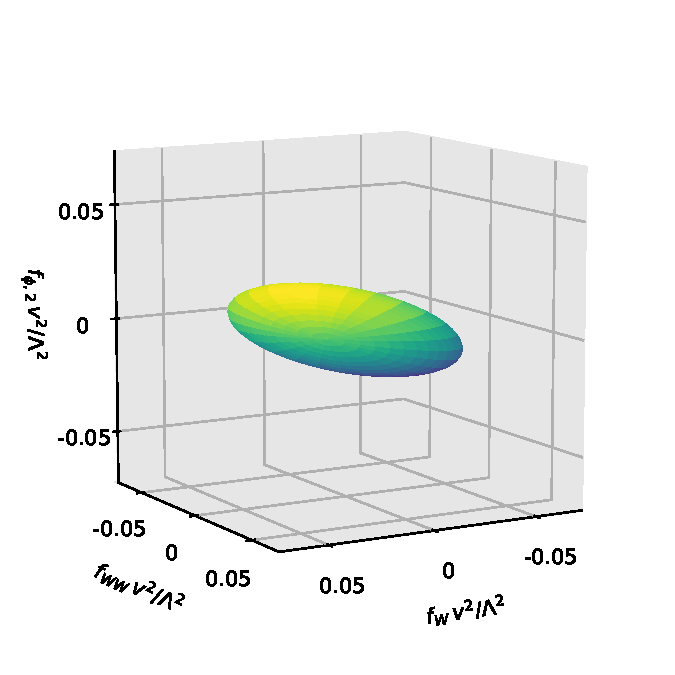
\includegraphics[width=0.49 \textwidth]{fig/information/wbf_tautau_3d_low}%
  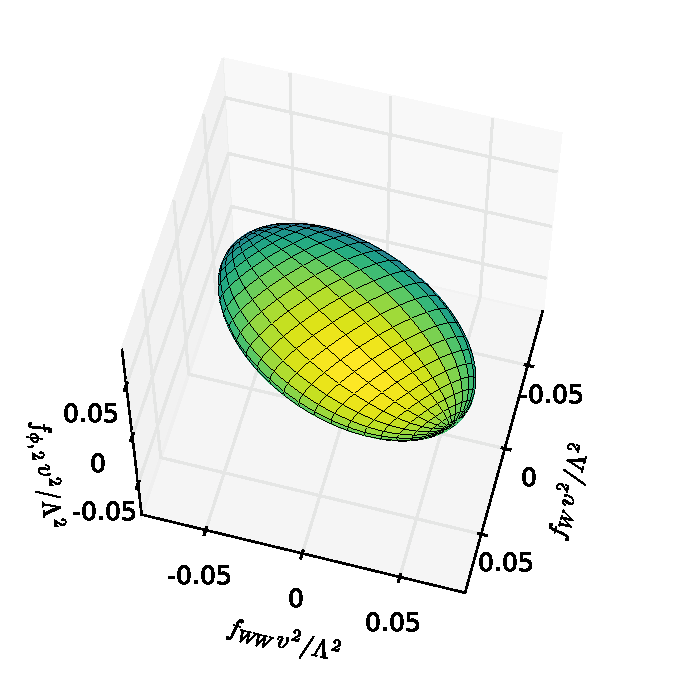
\includegraphics[width=0.49 \textwidth]{fig/information/wbf_tautau_3d_high}%
  \caption{Error ellipsoid defined by the Fisher information in the
    WBF $h \to \tau \tau$ channel through the contour
    $d_\text{local}(\boldtheta ; \boldzero) = 1$. The $\theta_i$ not
    shown are set to zero. The two panels show different views of the
    same ellipsoid.}
\label{fig:information_wbf_tautau_geometry_2d}
\end{figure}

These results show that the WBF process has quite different
sensitivities to the five operators: $\ope{\phi,2}$, which is the only
one that affects the decay vertex in addition to the production
process, can be most strongly constrained and is weakly correlated
with $\ope{W}$. An ideal measurement can probe this operator with a
precision of $\Delta \theta \approx 0.02$, translating into a maximal
new physics reach $\Lambda/\sqrt{f_{\phi,2}} \approx 1.9~\tev$. The
sensitivity to the strongly correlated $\ope{W}$-$\ope{WW}$ plane is
also quite large: these directions can be probed at the
$\Delta \theta \approx 0.05$ or
$\Lambda/\sqrt{f_{W/WW}} \approx 1~\tev$ level. Finally, $\ope{B}$ and
$\ope{BB}$ only play a role in subleading $Z$-mediated production
diagrams. Their Wilson coefficients cannot be measured very well in
this process, and does not affect the measurement of the other
operators through correlations.

In \autoref{fig:information_wbf_tautau_geometry_2d} we visualise the
sensitivity to the three operators $\ope{\phi,2}$, $\ope{W}$, and
$\ope{WW}$ as contours of the local information distances from the SM
as defined in \autoref{eq:information_local_distances}. Such an error
ellipsoid shows the maximum precision that can be attained in a
measurement in this process.

Moving away from the SM, the Fisher information and with it the
sensitivity to the different operators changes. The largest effects
are visible towards large positive (large negative) values of
$f_{\phi,2}$, where the expected cross section is much smaller
(larger) and theory parameters can be measured with smaller (larger)
precision. Following \autoref{eq:information_global_distances}, we
integrate infinitesimal distances along geodesics in theory space to
define global distances in the model parameter space. Unlike the local
distances, these take into account the curvature of the manifold, \ie
how the Fisher information changes with the theory
parameters. \autoref{fig:information_wbf_tautau_global_distances}
shows the resulting distances for a number of two-dimensional slices
in parameter space, confirming the large sensitivity to
$\ope{\phi,2}$, $\ope{W}$, and $\ope{WW}$.

\wbfpyramid{wbf_tautau_global}{fig:information_wbf_tautau_global_distances}
{Error ellipses defined by the Fisher information in the WBF
  $h \to \tau \tau$ channel. We show global distances from the SM
  $d(\boldtheta,\mathbf{0})$, where in each panel the $\theta_i$ not
  shown are set to zero. The white contours show distances of
  $d=1,2,3,4,5$.}

In \autoref{fig:information_wbf_tautau_local_vs_global} we compare the
global distances to the local distances defined in
\autoref{eq:information_local_distances}. This provides some insight
into the role of $\ord{1/\Lambda^4}$ effects, as discussed in
\autoref{sec:information_eft}.  At $d = 1,2$ the differences are
small, signalling that an optimal measurement will be dominated by the
linearised dimension-six amplitudes. On the other hand, analyses based
on less luminosity or requiring more stringent exclusion criteria
(translating into larger distances) will only probe new physics scales
closer to the electroweak scale, in which case the squared
dimension-six terms will have a larger effect.

\begin{figure}
  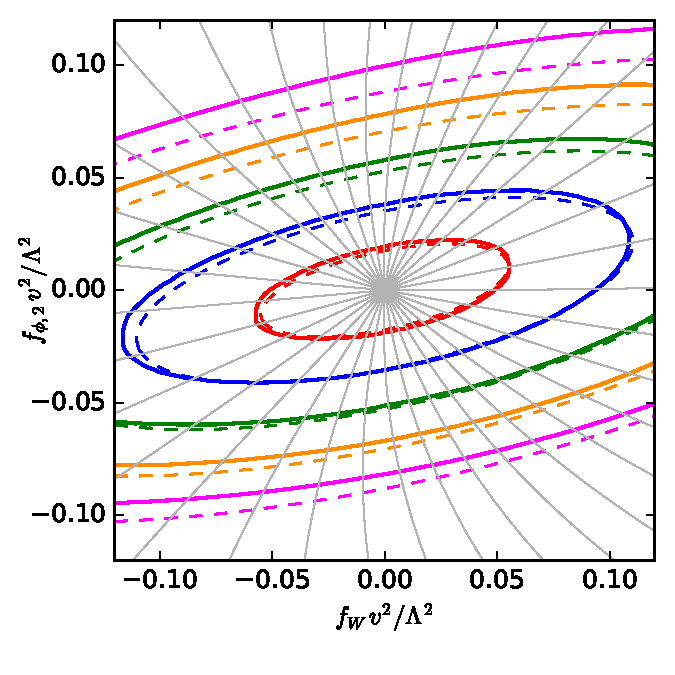
\includegraphics[width=0.33 \textwidth,clip,trim=0.3cm 0 0.05cm 0]{fig/information/wbf_tautau_geometry_fphi2_fw}%
  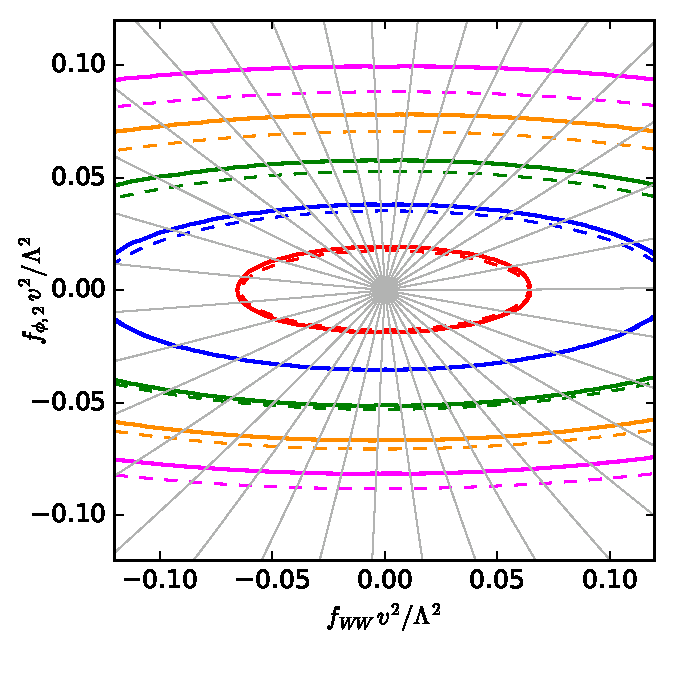
\includegraphics[width=0.33 \textwidth,clip,trim=0.3cm 0 0.05cm 0]{fig/information/wbf_tautau_geometry_fphi2_fww}%
  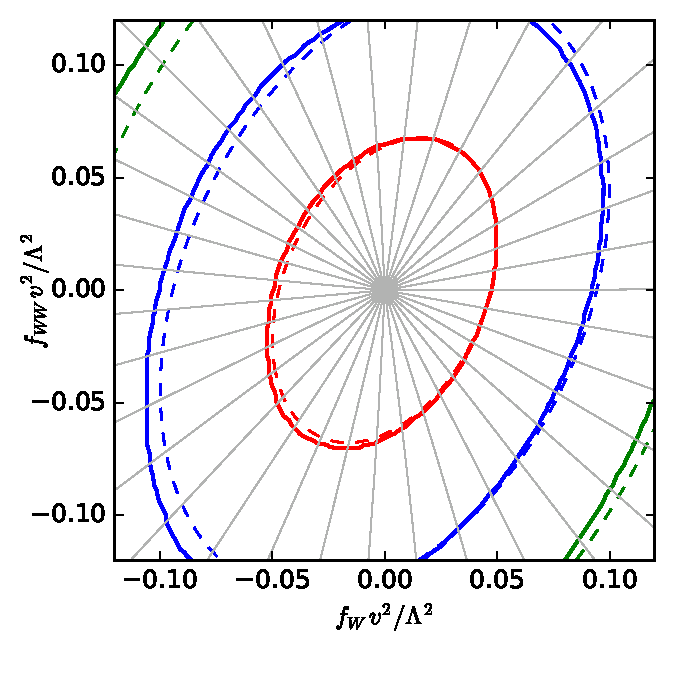
\includegraphics[width=0.33 \textwidth,clip,trim=0.3cm 0 0.05cm 0]{fig/information/wbf_tautau_geometry_fww_fw}%
  \caption{Error ellipses defined by the Fisher information in the WBF
    $h \to \tau \tau$ channel. We show contours of local distance
    $d_\text{local}(\boldtheta ; \boldzero)$ (dashed) and global distance
    $d(\boldtheta,\boldzero)$ (solid).  The coloured contours indicate
    distances of $d = 1,2,3,4,5$. In grey we show example geodesics. The
    $\theta_i$ not shown are set to zero. }
\label{fig:information_wbf_tautau_local_vs_global}
\end{figure}



%%%%%%%%%%%%%%%%%%%%%%%%%%%%%%%%%%%%%%%%%%%%%%%%%%%%%%%%%%%%
\subsubsection{Differential information}
%%%%%%%%%%%%%%%%%%%%%%%%%%%%%%%%%%%%%%%%%%%%%%%%%%%%%%%%%%%%

In a next step, we calculate the distribution of this information,
evaluated at the SM point $\boldtheta = \boldzero$, over phase
space. Following \autoref{sec:information_differential}, we calculate
the Fisher information in bins of kinematic variables. This set of
information matrices can be condensed into a single real-valued
function of the phase-space variables by calculating the
determinants. The resulting distribution of differential information
over typical kinematic variables is shown in
Figures~\ref{fig:information_wbf_tautau_differential_information_taus}
and \ref{fig:information_wbf_tautau_differential_information_jets} and
compared to the differential cross sections of the signal and the
dominant background process.

\begin{figure}
  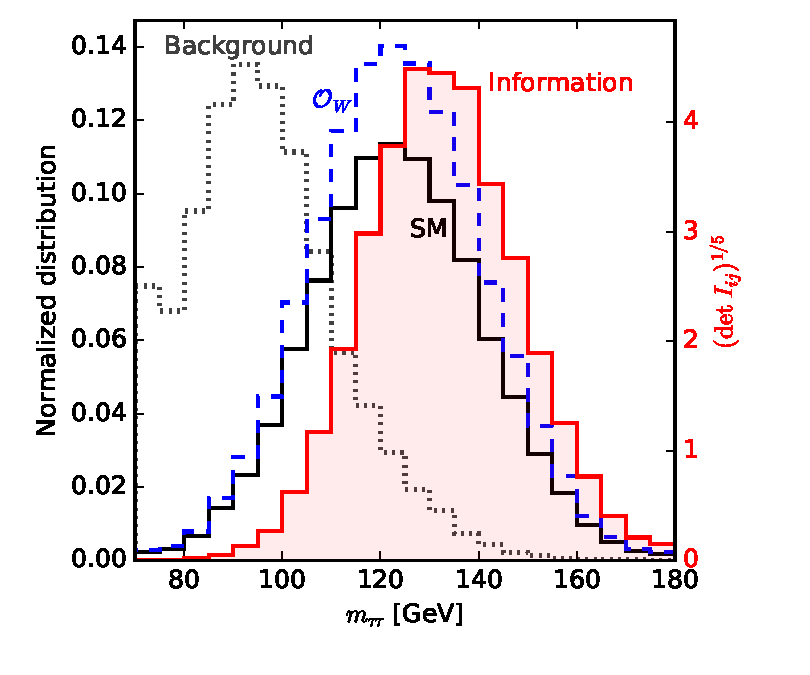
\includegraphics[width=0.49 \textwidth]{fig/information/wbf_tautau_information_over_mtautau}%
  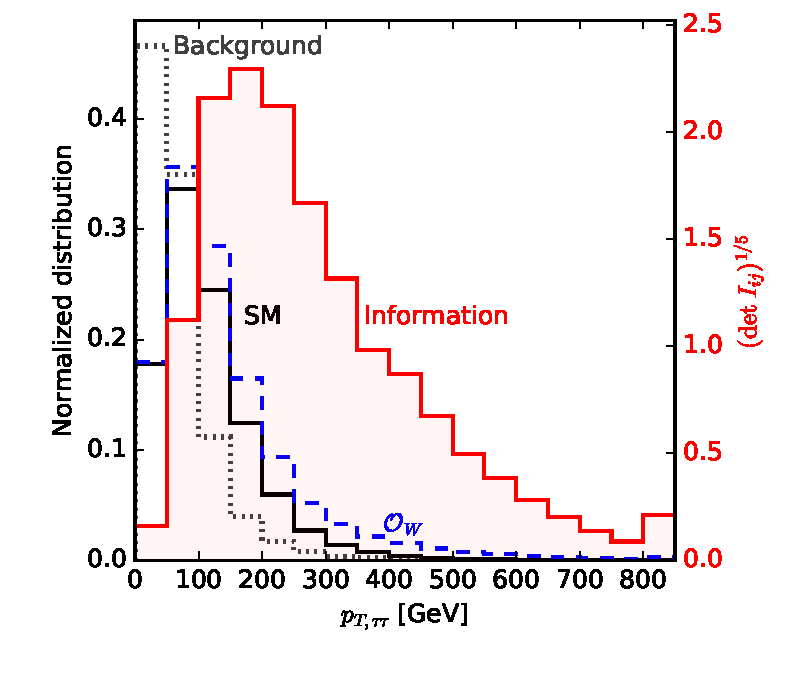
\includegraphics[width=0.49 \textwidth]{fig/information/wbf_tautau_information_over_pttautau}%
  \caption{Distribution of the differential Fisher information in the
    WBF $h \to \tau \tau$ channel (shaded red) with respect to the
    invariant mass of the $\tau \tau$ system (left) and its transverse
    momentum (right). We also show the normalised SM signal (solid
    black) and QCD $Z$+jets (dotted grey) rates. The dashed blue line
    shows the effect of an exaggerated
    $f_{W} \, v^2 / \Lambda^2 = 0.5$. The last bin is an overflow
    bin.}
  \label{fig:information_wbf_tautau_differential_information_taus}
\end{figure}

\begin{figure}
  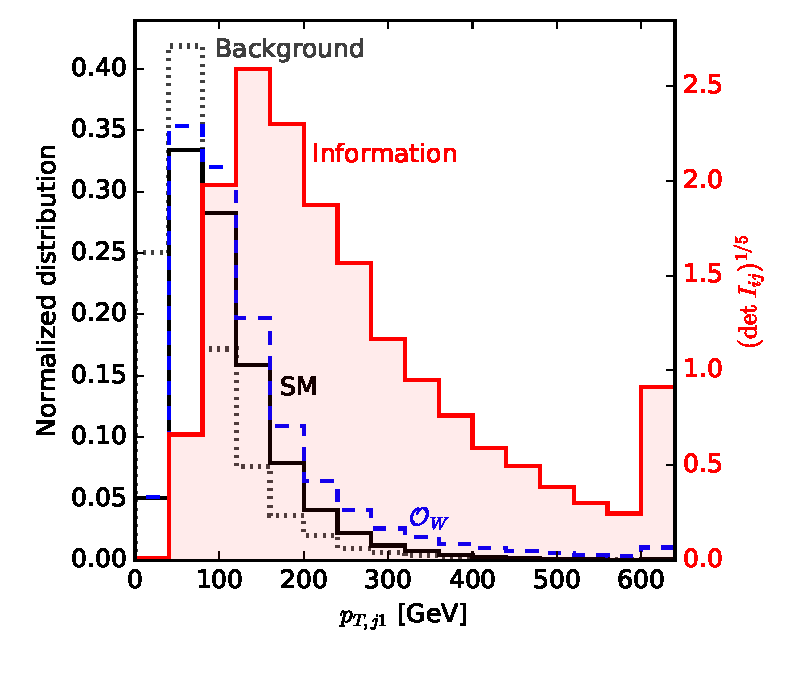
\includegraphics[width=0.49 \textwidth]{fig/information/wbf_tautau_information_over_ptj}%
  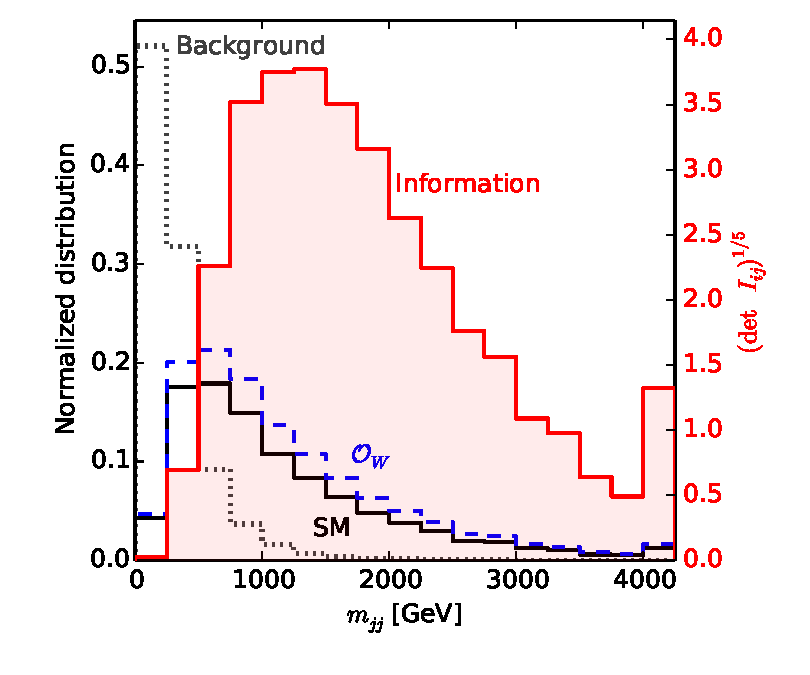
\includegraphics[width=0.49 \textwidth]{fig/information/wbf_tautau_information_over_mjj}\\%
  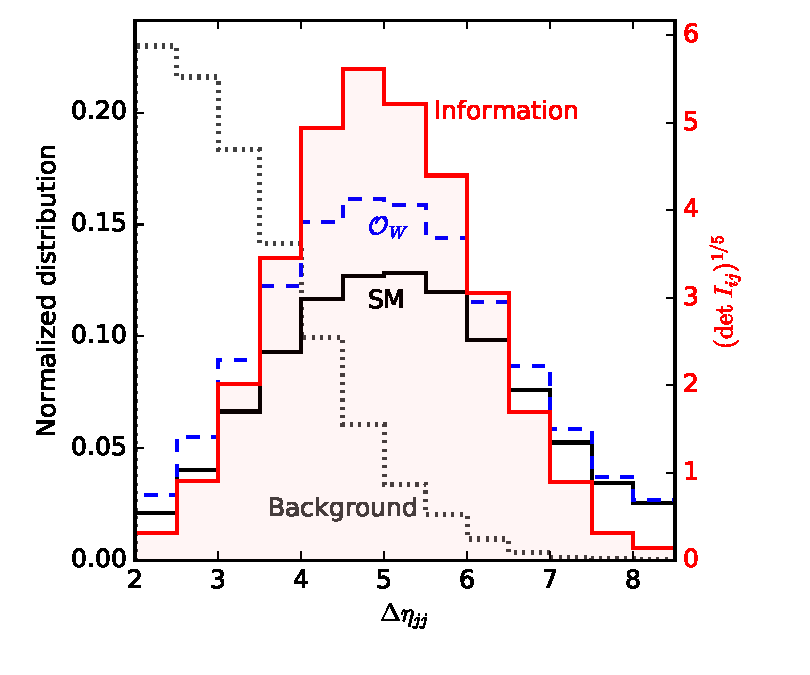
\includegraphics[width=0.49 \textwidth]{fig/information/wbf_tautau_information_over_deltaeta}%
  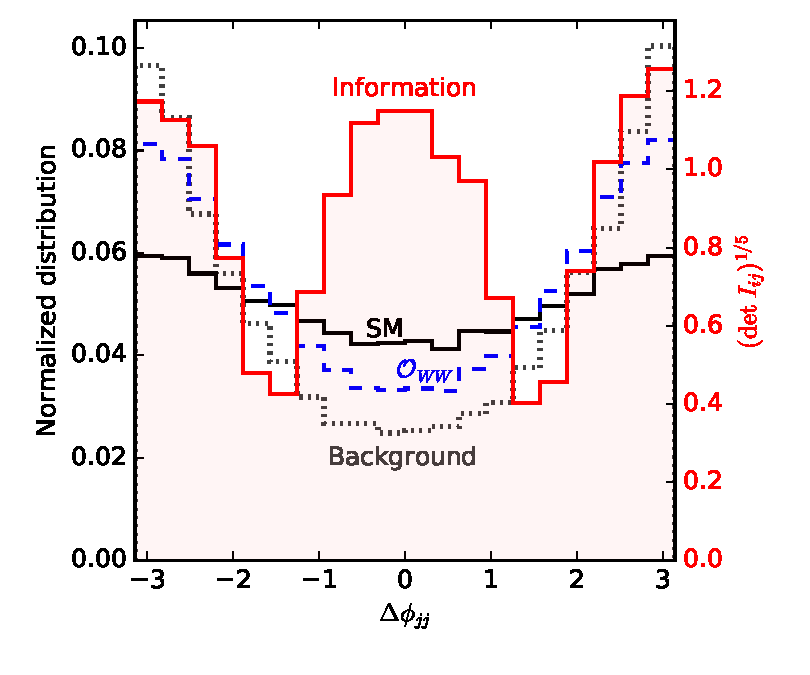
\includegraphics[width=0.49 \textwidth]{fig/information/wbf_tautau_information_over_deltaphi}%
  \caption{Distribution of the differential Fisher information in the
    WBF $h \to \tau \tau$ channel (shaded red) with respect to the
    transverse momentum of the leading jet (top left), the dijet mass
    (top right), the separation in pseudorapidity between the two jets
    (bottom left), and their difference in the azimuthal angle (bottom
    right). We also show the normalised SM signal (solid black) and
    QCD $Z$+jets (dotted grey) rates. The dashed blue line shows the
    effect of an exaggerated $f_{W} \, v^2 / \Lambda^2 = 0.5$, except
    in the bottom right panel, where we show
    $f_{WW} \, v^2 / \Lambda^2 = 0.5$. The last bin is an overflow
    bin.}
  \label{fig:information_wbf_tautau_differential_information_jets}
\end{figure}

Clearly, the signal-to-background ratio improves for large invariant
masses of the tagging jets and towards $m_{\tau \tau}$ values around
the Higgs mass. The information on all directions in model space is
larger in these phase-space regions. On the other hand, most of our
dimension-six operators include derivatives, leading to an increasing
amplitude with momentum transfer through the gauge-Higgs vertex. This
momentum flow is not observable, but the transverse momenta of the
tagging jets and the Higgs boson are strongly correlated with it, as
shown in \autoref{sec:validity_wbf_observables}. Indeed most of the
information on higher-dimensional operators comes from the high-energy
tail of the transverse momenta of the tagging jets or the $\tau \tau$
system, confirming what we demonstrated for specific model setups in
the previous chapter. Note that these distributions also quantify how
much the power of a Higgs measurement is limited by imposing an upper
limit on the momentum transfer to improve the validity of the EFT.

In the rapidity difference between the tagging jets we can see a
trade-off between these two effects: on the one hand, at larger
rapidity distances the signal-to-background ratio clearly
improves~\cite{Kleiss:1987cj, Baur:1990xe, Barger:1991ib,
  Rainwater:1996ud, Rainwater:1998kj, Cox:2010ug, Gerwick:2011tm}. On
the other hand, the largest effects from dimension-six operators appear
at smaller $\Delta \eta_{jj}$, again driven by the larger momentum
transfer~\cite{Biekotter:2016ecg}. In the bottom left panel of
\autoref{fig:information_wbf_tautau_differential_information_jets} we
see that most of the information on these operators comes from
$\Delta \eta_{jj} = 3\dots7$. Tight cuts with the aim to remove
backgrounds thus lose a sizeable fraction of the information on
dimension-six operators.

In practice, the distribution of the differential information can be a
useful tool to guide the design of event selections. As an example, we
consider traditional WBF cuts
%
\begin{equation}
  105~\gev < m_{\tau \tau} < 165~\gev  \,, \quad
  p_{T,j_1} > 50~\gev \,, \quad
  \Delta \eta_{jj} > \Delta \eta_{jj}^{\text{min}}
  \quad \text{and} \quad
  m_{jj} > m_{jj}^{\text{min}} \,.
\end{equation}
%
In \autoref{fig:information_wbf_tautau_cut_scan} we show how the
signal purity and the Fisher information depend on the choice of
$\Delta \eta_{jj}^{\text{min}}$ and $m_{jj}^{\text{min}}$. For a given
signal-to-background ratio we can pick cuts that maximise the Fisher
information, or vice versa, as demonstrated in the left panel of
\autoref{fig:information_wbf_tautau_cut_roc}.  This is somewhat
reminiscent of `receiver operating characteristic' (ROC) curves that
compare the efficiency for the SM Higgs signal to the background
rejection rate, as shown in the right panel of
\autoref{fig:information_wbf_tautau_cut_roc}. The information-based
analysis, however, takes into account the sensitivity of signal events
in different phase-space regions to new physics effects, which the ROC
curve is by design blind to.

\begin{figure}
  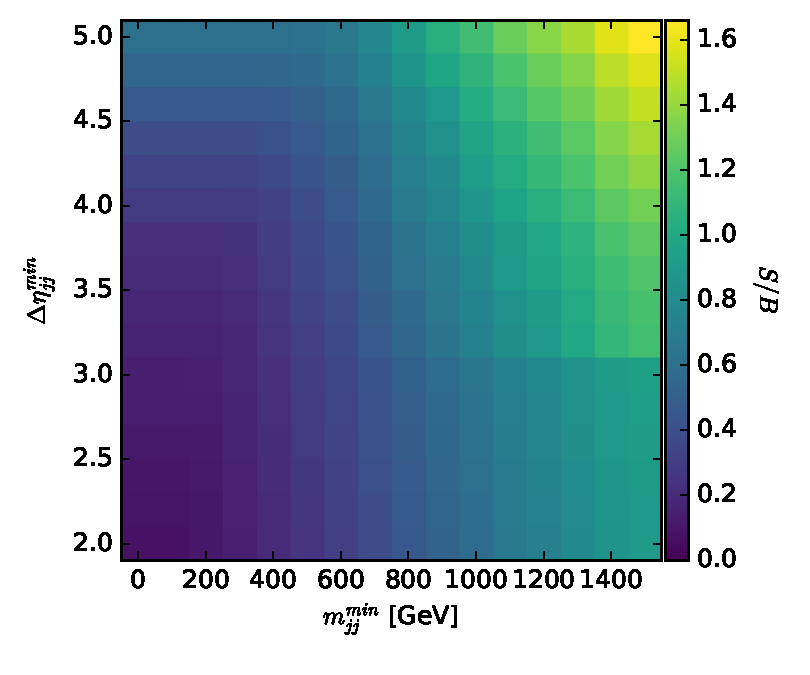
\includegraphics[width=0.49 \textwidth]{fig/information/wbf_tautau_tunecuts_purity}%
  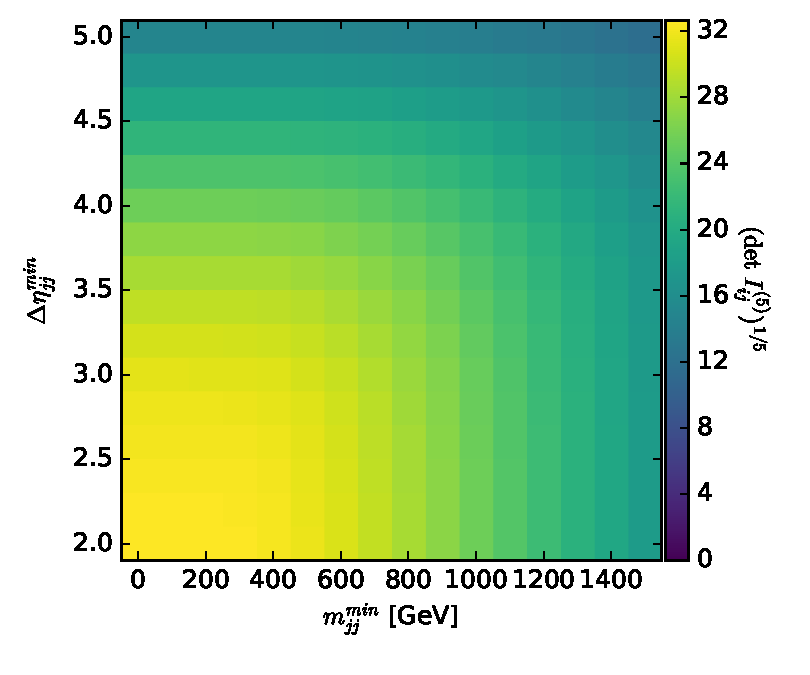
\includegraphics[width=0.49 \textwidth]{fig/information/wbf_tautau_tunecuts_information}%
  \caption{SM signal-to-background ratio (left) and determinant of the
    Fisher information (right) in the WBF $h \to \tau \tau$ channel as
    a function of the WBF cuts
    $\Delta \eta_{jj} > \Delta \eta_{jj}^{\text{min}}$ and
    $m_{jj} > m_{jj}^{\text{min}}$.}
  \label{fig:information_wbf_tautau_cut_scan}
\end{figure}

\begin{figure}
  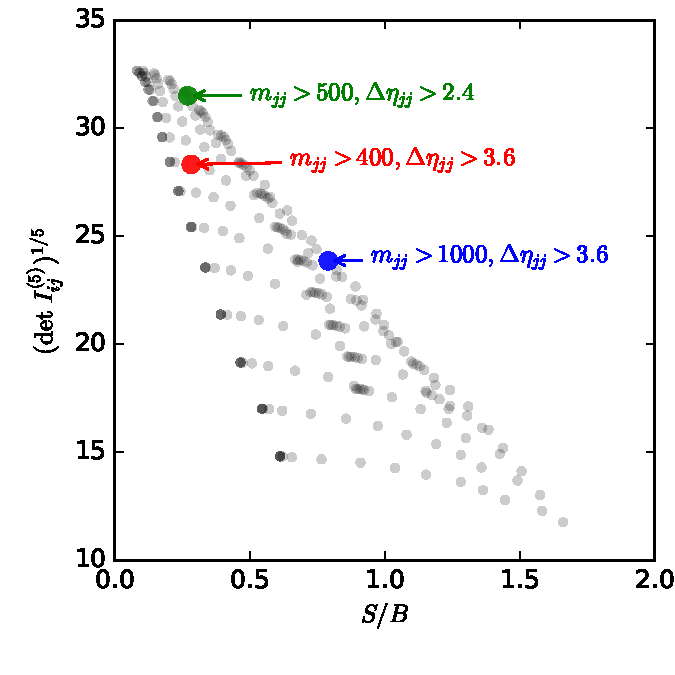
\includegraphics[width=0.49 \textwidth]{fig/information/wbf_tautau_tunecuts_purity_vs_information}%
  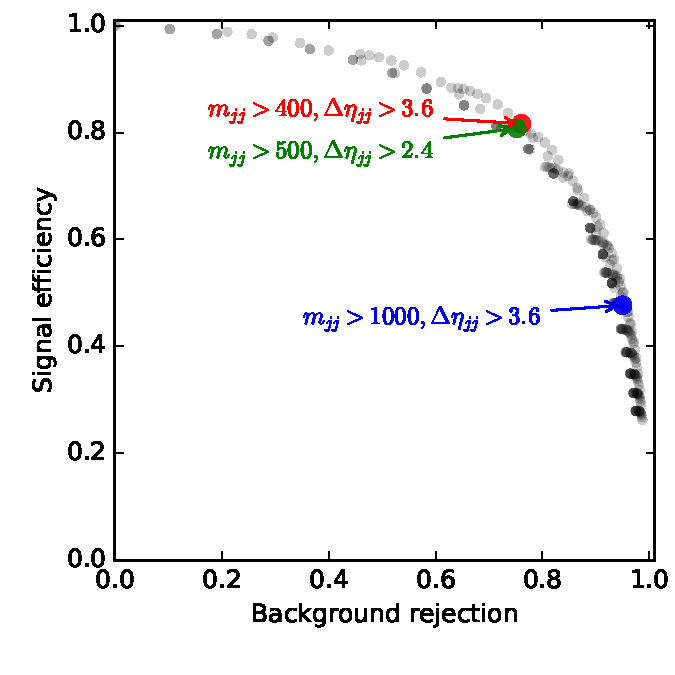
\includegraphics[width=0.49 \textwidth]{fig/information/wbf_tautau_tunecuts_roc}%
  \caption{Trade-off between signal purity and information in the WBF
    $h \to \tau \tau$ channel for different WBF cuts. Left:
    determinant of the Fisher information vs.\ signal-to-background
    ratio. Right: signal efficiency vs.\ background rejection,
    calculated after the common cuts
    $105~\gev < m_{\tau \tau} < 165~\gev$ and $p_{T,j1} >
    50~\gev$. The coloured dots show three example selections.}
  \label{fig:information_wbf_tautau_cut_roc}
\end{figure}

\newparagraph
%
The distribution of the differential Fisher information also provides
us with another perspective on the EFT validity discussed in the
previous chapter. There we demonstrated that the effective model can
break down in the high-energy tail of distributions, and concluded that
an additional analysis with cuts that impose a maximum momentum
transfer can improve the applicability of the EFT. For weak boson
fusion, this means requiring
%
\begin{equation}
  p_{T,j} < p_{T,j}^{\text{max}} \,,
  \label{eq:information_ptmax_cut}
\end{equation}
%
as shown in \autoref{sec:validity_wbf_observables}.

Our tools let us calculate the Fisher information in the WBF
$h \to \tau \tau$ channel for different cuts of the form
\autoref{eq:information_ptmax_cut}. For simplicity, we focus on the
operators $\ope{W}$ and $\ope{WW}$ and calculate the determinant of
the Fisher information in this plane. Following
\autoref{eq:information_new_physics_reach}, we translate it into a
typical new physics reach
%
\begin{equation}
  \frac \Lambda {\sqrt{f}} = v \; \sqrt{\det I_{ij}(\boldzero)}^{1/4} 
  \label{eq:information_scales_reach}
\end{equation}
%
of an optimal measurement. For universal Wilson coefficients
$f_W = f_{WW} \equiv f$, we can calculate the new physics reach
$\Lambda$ and compare it to the maximum momentum transfer
$p_{T,j}^{\text{max}}$.

\begin{figure}
  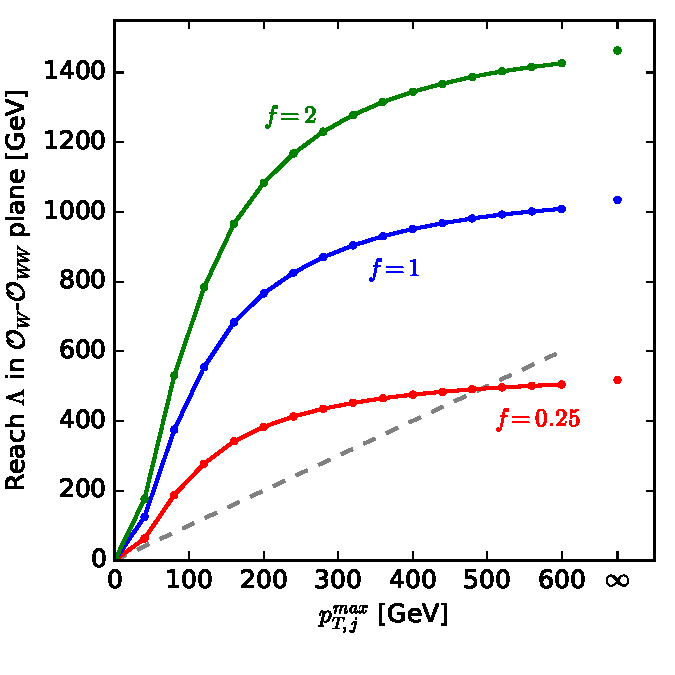
\includegraphics[width=0.49 \textwidth]{fig/information/wbf_tautau_scales}%
  \caption{Maximal new physics reach of the WBF $h\to \tau \tau$
    channel in the $\ope{W}$-$\ope{WW}$ plane as a function of an
    upper cut of the transverse jet momenta
    $p_{T,j}^{\text{max}}$. The green, blue, and red curves show the
    optimal reach for different values for universal Wilson
    coefficients $f_W = f_{WW} \equiv f$, as defined in
    \autoref{eq:information_scales_reach}. The dashed grey line
    sketches the maximum momentum transfer in the events, assuming
    that this is accurately captured by the jet $p_T$.}
  \label{fig:information_wbf_tautau_scales}
\end{figure}

\autoref{fig:information_wbf_tautau_scales} shows that for strongly
coupled physics we can probe new physics scales significantly above
the experimental momentum transfer, at least in our simple setup that
neglects systematic and theory uncertainties. Such a scenario does not
require any cuts of the form in \autoref{eq:information_ptmax_cut} for
the EFT to work. However, for moderate to small Wilson coefficients
$0.25 \lesssim f \lesssim 1$, the scale hierarchy is less clear,
confirming the discussion in
Section~\ref{sec:validity_introduction}. Our results show that
imposing a maximum momentum transfer of a few hundred GeV can increase
the separation between the experimental energy scale and the probed
new physics scales, and thus the usefulness of the effective theory.



%%%%%%%%%%%%%%%%%%%%%%%%%%%%%%%%%%%%%%%%%%%%%%%%%%%%%%%%%%%%
\subsubsection{Information in distributions}
%%%%%%%%%%%%%%%%%%%%%%%%%%%%%%%%%%%%%%%%%%%%%%%%%%%%%%%%%%%%

While this total Fisher information based on the full kinematics
provides us with optimal experimental results, it remains to be shown
that we can access it in practice. Matrix-element-based
methods~\cite{Kondo:1988yd, Abazov:2004cs, Gao:2010qx, Alwall:2010cq,
  Avery:2012um, Andersen:2012kn, Campbell:2013hz, Artoisenet:2013vfa,
  Martini:2015fsa, Gritsan:2016hjl, Soper:2011cr, Soper:2012pb,
  Soper:2014rya, Atwood:1991ka, Davier:1992nw, Diehl:1993br} and
recent proposals using machine learning for high-dimensional
likelihood fits~\cite{Cranmer:2015bka, Cranmer:2016lzt} aim to tackle
exactly this problem. Still, a relevant question is how much of this
maximum information is retained in simple one-dimensional or
two-dimensional distributions of standard kinematic observables
$\mathbf{v}$. On the one hand, this lets us assess the potential of
traditional histogram-based analysis methods and compare it to the
optimal results discussed before. On the other hand, the information
in kinematic distributions provides a ranking of the most useful
observables that experimentalists should measure and publish, for
instance to be used in recasted analyses or in global fits by
theorists~\cite{Corbett:2015ksa, Butter:2016cvz}.

In the presence of backgrounds, a histogram-based analysis requires a
stringent event selection, either based on traditional kinematic cuts
or on a multivariate classifier. First, we choose the WBF cuts
%
\begin{align}
  105~\gev < m_{\tau \tau} < 165~\gev \,, \quad
  p_{T,j_1} > 50~\gev \,, \quad
  m_{jj} > 1~\tev \quad \text{and} \quad
  \Delta \eta_{jj} > 3.6 \,.
  \label{eq:information_wbf_tautau_wbfcuts}
\end{align}
%
As shown in \autoref{fig:information_wbf_tautau_cut_roc}, this
improves the signal-to-background ratio to nearly unity, though at the
cost of losing discrimination power. An analysis would profit from an
optimisation of these cuts, but this goes beyond the scope of our
demonstration. Based on this selection, we analyse the distributions
of the following standard observables:
%
\begin{itemize}
\item the transverse momentum of the leading $\tau$, $p_{T,\tau_1}$,
  with bin size $25~\gev$ up to $500~\gev$ and an overflow bin;
%
\item the invariant mass of the $\tau \tau$ system, $m_{\tau \tau}$,
  with bin size $5~\gev$ in the allowed range of
  $105~\gev < m_{\tau\tau} <165~\gev$;
%
\item the transverse momentum of the $\tau \tau$ system,
  $p_{T,\tau \tau}$, with bin size $50~\gev$ up to $800~\gev$ and an
  overflow bin;
%
\item the transverse momentum of the leading jet, $p_{T,j_1}$, with bin
  size $50~\gev$ up to $800~\gev$ and an overflow bin;
%
\item the invariant mass of the dijet system, $m_{jj}$, with bin size
  $250~\gev$ up to $4~\tev$ and an overflow bin;
%
\item the separation in pseudorapidity between the two jets,
  $\Delta \eta_{jj}$, with bin size $0.5$ up to $8.0$ and an overflow
  bin;
%
\item the separation in azimuthal angle between the two jets, now
  defined in a signed version~\cite{Klamke:2007cu}
  $\Delta \phi_{jj} = \phi_{j_{\eta < 0}} - \phi_{j_{\eta >0}}$, with
  bin size $2 \pi / 20$;
%
\item the separation in pseudorapidity between the $\tau \tau$ system
  and the leading jet, $\Delta \eta_{\tau\tau, j1}$, with bin size $0.5$
  up to $8.0$ and an overflow bin; and
%
\item the separation in azimuthal angle between the $\tau \tau$ system
  and the leading jet, $\Delta \phi_{\tau \tau, j1}$, with bin size
  $\pi / 10$.
\end{itemize}

\begin{figure}
  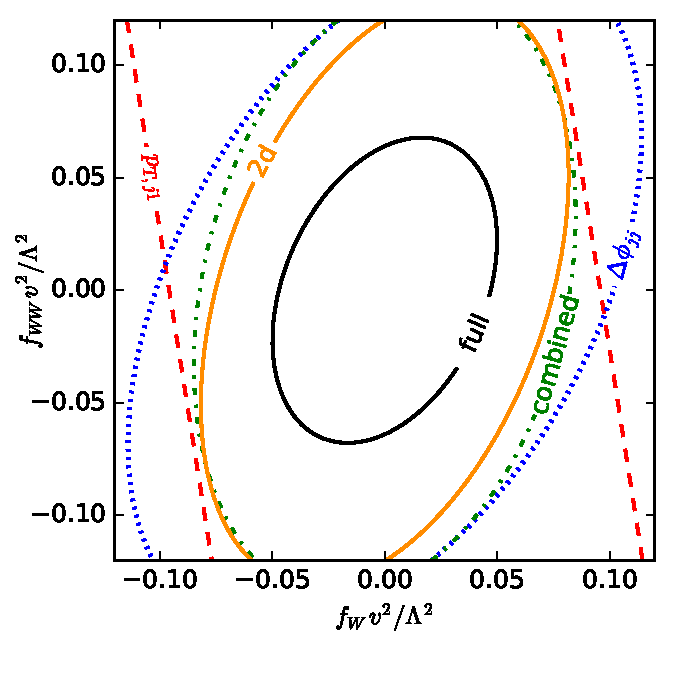
\includegraphics[width=0.49 \textwidth]{fig/information/wbf_tautau_histos_contours}
  \caption{Information from histograms compared to the full
    information  (black) in the WBF $H \to \tau \tau$ channel, shown as contours
    $\dlocal(\boldtheta ; \boldzero) = 1$. We include
    $p_{T,j_1}$, $\Delta \phi_{jj}$, their naive combination assuming
    no mutual information, and their two-dimensional histogram. The
    $\theta_i$ not shown are set to zero.}
  \label{fig:information_wbf_tautau_histograms_contours}
\end{figure}

In \autoref{fig:information_wbf_tautau_histograms_contours}, we compare
the error ellipses expected from the analysis of a few of these
distributions. Measures of the momentum transfer such as the
transverse momentum of the leading tagging jet mostly constrain
$\ope{W}$, while angular correlations between the jets are more
sensitive to $\ope{WW}$. Stringent constraints on the full operator
space can be achieved by combining the information in these
distributions. A fully correlated two-dimensional histogram carries
slightly more information than a combination of the one-dimensional
histograms following
\autoref{eq:information_combined_information_distributions}.

Finally, we compare the information in all of the above distributions
in \autoref{fig:information_wbf_tautau_histograms_comparison}. The top
panel shows the eigenvalues of the individual information matrices,
and the colours indicate which operators the corresponding
eigenvectors are composed of. This allows us to see which
distributions measure which directions in theory space well, and where
blind directions arise. 

\begin{figure}
  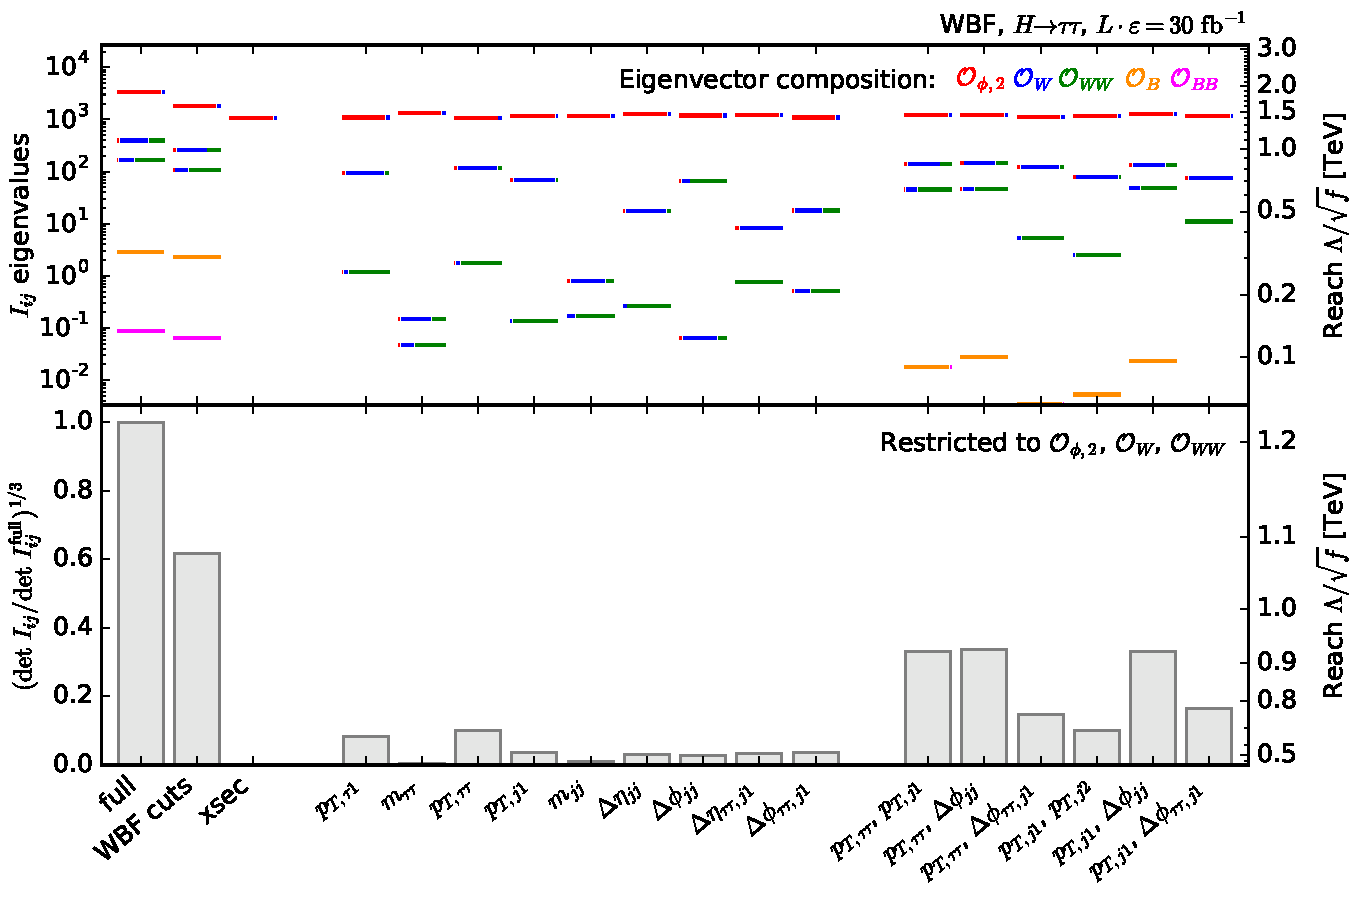
\includegraphics[width=\textwidth]{fig/information/wbf_tautau_histos_comparison}
  \caption{Total Fisher information for the WBF $h \to \tau \tau$
    channel (`full'), Fisher information after the cuts in
    \autoref{eq:information_wbf_tautau_wbfcuts}, and the information
    in several distributions after this selection.  The top panel
    shows the eigenvalues, the colours denote the composition of the
    corresponding eigenvectors. The right axis translates the
    eigenvalues into a new physics reach for the corresponding
    combination of Wilson coefficients.  In the bottom panel we show
    the determinants of the Fisher information restricted to
    $\ope{\phi,2}$, $\ope{W}$, and $\ope{WW}$, normalised to the full
    information. Again, the right axis translates them into a new
    physics reach.}
\label{fig:information_wbf_tautau_histograms_comparison}
\end{figure}

The lower panel shows the determinants of the Fisher information
matrices. We restrict this analysis to the space spanned by the three
operators $\ope{\phi,2}$, $\ope{W}$, and $\ope{WW}$ to avoid results
that strongly depend on the other two operators, which cannot be
measured reliably in this process anyway. These determinants provide a
straightforward measure of the information in distributions that is
independent of EFT basis rotations, see \autoref{sec:information_eft}.

In general, one-dimensional histograms of single observables probe
individual directions in phase space well, but always suffer from
basically blind directions. To maximise the constraining power on all
operators, we need to combine measures of momentum transfer such as the
jet or $\tau \tau$ transverse momenta on the one hand with jet angular
correlations on the other hand. Even then there is a substantial
difference to the maximum information in the process: the combined
analysis of jet transverse momenta and $\Delta \phi_{jj}$ has a new
physics reach $\Lambda / \sqrt{f}$ in the
$\ope{\phi,2}$-$\ope{W}$-$\ope{WW}$ space of $0.9~\tev$, compared to
$1.2~\tev$ for the full kinematics. Under our
simplistic assumptions this corresponds to roughly three times as much
data.  Half of this loss in constraining power is due to information
in background-rich regions discarded by the WBF cuts, the other half is due
to non-trivial kinematics not captured by the double differential
distributions.

\newparagraph
%
In the light of the large amount of information discarded by the WBF
cuts in \autoref{eq:information_wbf_tautau_wbfcuts}, we repeat this
comparison with an alternative matrix-element-based event
selection. Instead of cutting on standard kinematic observables, we
select all events in `signal-like' phase-space regions, defined as
those with a larger expected SM WBF rate than the combined expected
background rates,
%
\begin{equation}
  \frac{\sigma_{\text{SM WBF}}\;f^{(1)}(\boldx|\text{SM WBF})}{\sigma_{\text{backgrounds}}\;f^{(1)} (\boldx|\text{backgrounds})}
  = \frac{\Delta \sigma_\text{SM WBF}(\boldx)}{\Delta \sigma_\text{backgrounds} (\boldx)}
  > 1 \,.
  \label{eq:information_wbf_tautau_likelihoodcuts}
\end{equation}
%
We then calculate the information in the same distributions as before. 

\begin{figure}
  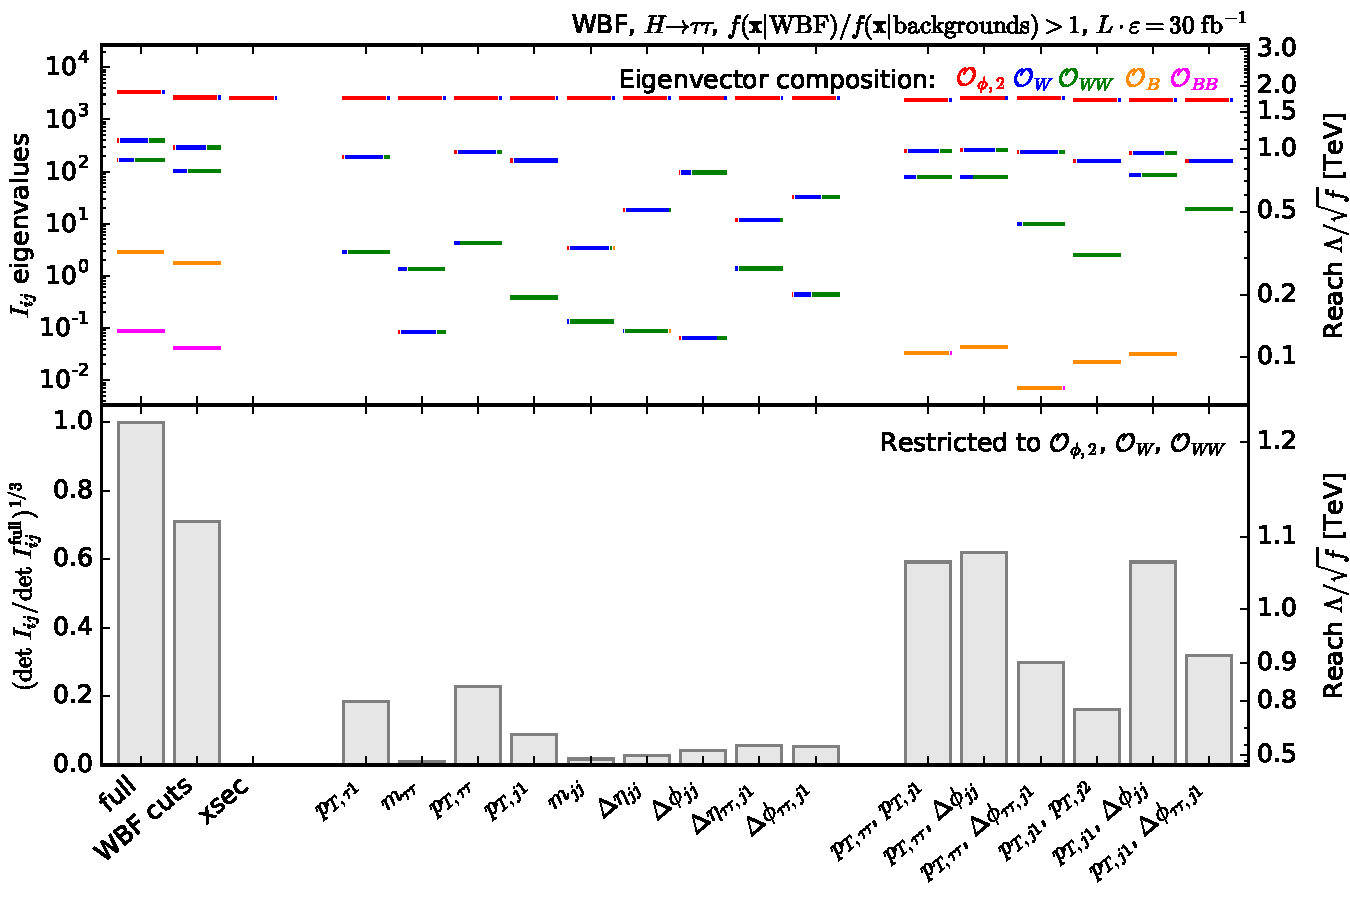
\includegraphics[width=\textwidth]{fig/information/wbf_tautau_histos_comparison_likelihoodcut}
  \caption{Total Fisher information for the WBF $h \to \tau \tau$
    channel (`full'), information after the matrix-element-based WBF
    cuts in \autoref{eq:information_wbf_tautau_likelihoodcuts}, and
    the information in several distributions after this
    selection. Except for the event selection, the plot is analogous
    to \autoref{fig:information_wbf_tautau_histograms_comparison}.}
\label{fig:information_wbf_tautau_histograms_comparison_likelihoodcut}
\end{figure}

As shown in
\autoref{fig:information_wbf_tautau_histograms_comparison_likelihoodcut},
the cut in \autoref{eq:information_wbf_tautau_likelihoodcuts} defines
a sample with little background contamination without sacrificing much
discrimination power. One-dimensional and two-dimensional
distributions can extract information on the operators more reliably
than after the kinematic event selection in
\autoref{eq:information_wbf_tautau_wbfcuts}. A combined measurement of
the jet transverse momenta and $\Delta \phi_{jj}$ is now able to probe
new physics scales of up to $1.1~\tev$ compared to $1.2~\tev$ for the
fully multivariate approach, corresponding to $70\%$ more data.



% %%%%%%%%%%%%%%%%%%%%%%%%%%%%%%%%%%%%%%%%%%%%%%%%%%%%%%%%%%%%
% \subsubsection{Summary}
% %%%%%%%%%%%%%%%%%%%%%%%%%%%%%%%%%%%%%%%%%%%%%%%%%%%%%%%%%%%%

% In our first application of information geometry to Higgs physics we
% demonstrated that weak boson fusion with a decay into tau pairs can
% ideally probe $\ope{\phi,2}$, $\ope{W}$, and $\ope{WW}$ at the
% $\Lambda / \sqrt{f} \sim 1.2~\tev$ level early during Run~2 of the
% LHC. As expected, a large fraction of this constraining power comes
% from the few events with large momentum transfer. Care has to be taken
% with standard cuts on $\Delta \eta_{jj}$, which unnecessarily limit
% the information in this process.

% Due to the sizeable backgrounds and the intricate phase-space
% structure of the signatures, traditional analysis methods based on
% tight kinematic cuts and standard observables struggle to extract all
% of this information. A matrix-element based event selection followed
% by a combined analysis of transverse jet momenta and jet angular
% correlations performs better, but still requires $70\%$ more data to
% probe the dimension-six operators on the same leven as an ideal, fully
% multivariate analysis.



%%%%%%%%%%%%%%%%%%%%%%%%%%%%%%%%%%%%%%%%%%%%%%%%%%%%%%%%%%%%
\subsection{Weak-boson-fusion Higgs to four leptons}
\label{sec:information_wbf_4l}
%%%%%%%%%%%%%%%%%%%%%%%%%%%%%%%%%%%%%%%%%%%%%%%%%%%%%%%%%%%%

With a thorough understanding of the WBF production process, we now
ask how much information a non-trivial decay mode
$h \to ZZ^* \to 4 \ell$ with $\ell = e, \mu$ adds. For this
particularly clean channel, shown in
\autoref{fig:information_wbf_4l_diag}, the backgrounds are not the
limiting factor, so we omit them for our toy study: a calculation with
\toolfont{MadGraph~5} shows that in the relevant phase-space region
the cross section of the dominant irreducible $ZZ^* \,jj$ background
is more than one order of magnitude smaller than the SM Higgs signal. This
also allows us to avoid smearing the $m_{4\ell}$ distribution. Again,
we restrict our initial study to the parton level and leading order.

\begin{figure}
  \fmfframe(0,15)(15,15){ %(L,T) (R,B)
    \begin{fmfgraph*}(150,70)
      \feynmansetup
      \fmfleft{i2,i1}
      \fmfright{o6,o5,o4,o3,o2,o1}
      \fmflabel{\small $q$}{i1}
      \fmflabel{\small $q$}{i2}
      \fmflabel{\small $q$}{o1}
      \fmflabel{\small $\ell^+$}{o2}
      \fmflabel{\small $\ell^-$}{o3}
      \fmflabel{\small $\ell^+$}{o4}
      \fmflabel{\small $\ell^-$}{o5}
      \fmflabel{\small $q$}{o6}
      \fmf{fermion,tension=4}{i1,v3}
      \fmf{fermion,tension=4}{i2,v4}
      \fmf{fermion,tension=2.5}{v3,o1}
      \fmf{fermion,tension=2.5}{v4,o6}
      \fmf{wiggly,label=\small $W$,, $Z$,label.side=right}{v3,v5}
      \fmf{wiggly,label=\small $W$,, $Z$,label.side=left}{v4,v5}
      \fmf{dashes,label=\small $h$,tension=0.5}{v5,v6}
      \fmf{wiggly,tension=0.3,label=\small $Z$,tension=0.3,label.side=right}{v7,v6}
      \fmf{wiggly,tension=0.3,label=\small $Z$,tension=0.3,label.side=right}{v6,v8}
      \fmf{fermion,tension=0.2}{o2,v7,o3}
      \fmf{fermion,tension=0.2}{o4,v8,o5}
      \fmfv{decoration.shape=circle,foreground=(0.8,,0.,,0.),decoration.size=5}{v5,v6}
    \end{fmfgraph*}
  }
  \caption[Feynman diagram for WBF Higgs production in the $4 \ell $
  mode]{Feynman diagram for WBF Higgs production in the $4 \ell $
    mode. The red dots show the Higgs-gauge interactions affected by
    the dimension-six operators of our analysis.}
  \label{fig:information_wbf_4l_diag}
\end{figure}

Requiring only minimal acceptance cuts
%
\begin{align}
  p_{T,j} &> 20 \ \gev \,,  &  |\eta_{j}| &< 5.0 \,, \notag \\ 
  p_{T,\ell} &> 10 \ \gev \,, &  |\eta_{\ell}| &< 2.5 \, ,
  \label{eq:information_wbf_4l_acceptance_cuts}
\end{align}
%
we calculate the Fisher information for $pp$ collision at
$\sqrt{s} = 13~\tev$. We now assume an increased integrated luminosity
of
%
\begin{equation}
  L \cdot \varepsilon = 100~\ifb \,,
\end{equation}
%
where $\varepsilon$ again refers to the combined particle
identification and trigger efficiencies. The SM cross section after
our selection cuts is 0.36~fb, corresponding to 36 expected events.

The relevant dimension-six operators are the same as in the $\tau \tau$
channel, and we again parametrise the model space with
\autoref{eq:information_model_parameters_wbf}. All other details
follow the setup in the previous section.



%%%%%%%%%%%%%%%%%%%%%%%%%%%%%%%%%%%%%%%%%%%%%%%%%%%%%%%%%%%%
\subsubsection{Total Fisher information}
%%%%%%%%%%%%%%%%%%%%%%%%%%%%%%%%%%%%%%%%%%%%%%%%%%%%%%%%%%%%

The full Fisher information at the SM for this process is
%
\begin{align}
  I_{ij} (\boldzero) =
\begin{pmatrix*}[r]
  144.3 & -27.3 & -11.5 & -1.6 & -0.7 \\
  -27.3 & 50.9 & -9.1 & 6.7 & -0.2 \\
  -11.5 & -9.1 & 36.9 & -1.2 & 1.0 \\
  -1.6 & 6.7 & -1.2 & 1.9 & -0.1 \\
  -0.7 & -0.2 & 1.0 & -0.1 & 0.1
\end{pmatrix*} \,,
\end{align}
%
with the eigenvectors, eigenvalues, and corresponding new physics reach 
%
\begingroup%
\allowdisplaybreaks%
\begin{align}
  \boldtheta_1 &= \fivevecr {0.96} {-0.25} {-0.08} {-0.02} {0.00} \,:
  & I_1 &= 152.4
  &&\leftrightarrow
  & \left( \frac {\Lambda} {\sqrt{f}} \right)_1 &= 864~\gev \,, \notag \\
  %
  \boldtheta_2 &= \fivevecr {-0.16} {-0.79} {0.58} {-0.11} {0.02} \,:
  & I_2 &= 52.8
  &&\leftrightarrow
  & \left( \frac {\Lambda} {\sqrt{f}} \right)_2 &= 663~\gev \,, \notag \\
  %
  \boldtheta_3 &= \fivevecr {0.21} {0.54} {0.81} {0.09} {0.02} \,:
  & I_3 &= 27.8
  &&\leftrightarrow
  & \left( \frac {\Lambda} {\sqrt{f}} \right)_3 &= 565~\gev \,, \notag \\
  %
  \boldtheta_4 &= \fivevecr {0.02} {0.14} {0.01} {-0.99} {0.04} \,:
  & I_4 &= 1.0
  &&\leftrightarrow
  & \left( \frac {\Lambda} {\sqrt{f}} \right)_4 &= 246~\gev \,, \notag \\
  %
  \boldtheta_5 &= \fivevecr {0.00} {0.00} {-0.03} {0.04} {1.00} \,:
  & I_5 &= 0.0
  &&\leftrightarrow
  & \left( \frac {\Lambda} {\sqrt{f}} \right)_5 &= 114~\gev \,. 
\end{align}%
\endgroup

The Fisher information approach allows us to directly compare this
outcome to the information in the $h\to \tau \tau$ channel in
\autoref{eq:information_wbf_tautau_information_sm}, or to calculate
the combined information in these two channels by simply adding their
Fisher information matrices after rescaling them to the same
luminosity. Clearly, the $\tau \tau$ channel contains significantly
more information on all operators. The decay $h \to 4\ell$ does not
even increase the sensitivity to $\ope{B}$ or $\ope{BB}$, both
are still basically blind directions.

\wbfpyramid{wbf_4l_global}{fig:information_wbf_4l_global_distances}
{Error ellipses defined by the Fisher information in the WBF
  $h \to 4\ell$ channel. We show global distances from the SM
  $d(\boldtheta,\mathbf{0})$, where in each panel the $\theta_i$ not
  shown are set to zero. The white contours show distances of
  $d=1,2,3,4,5$.}

Again we calculate global distances between theory points along
geodesics and show them in
\autoref{fig:information_wbf_4l_global_distances}. Local and global
distances are compared in \autoref{fig:information_wbf_4l_geometry},
with larger differences than in the $h \to \tau \tau$ channel. This is
because the tiny $h \to 4\ell$ branching fraction decreases the new
physics reach and with it the hierarchy of scales in our effective
Lagrangian, making the squared dimension-six amplitudes numerically
more relevant.

\begin{figure}
  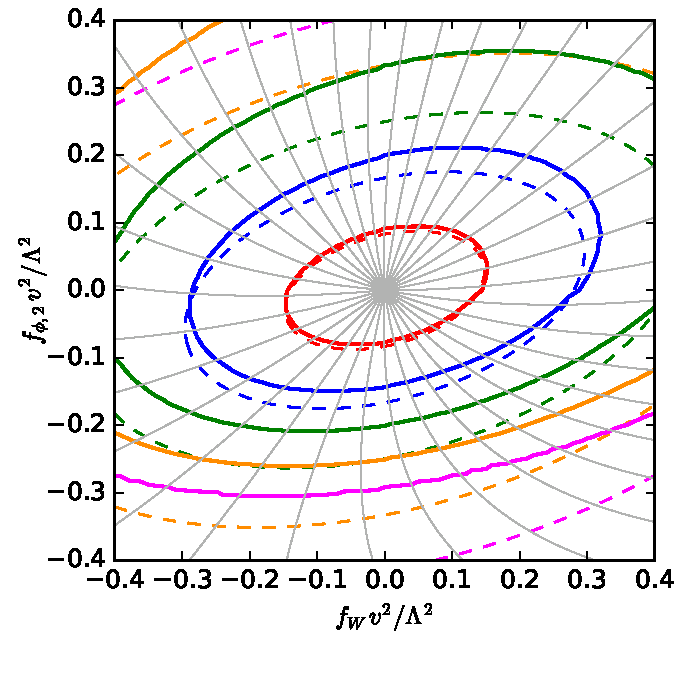
\includegraphics[width=0.33 \textwidth,clip,trim=0.3cm 0 0.05cm 0]{fig/information/wbf_4l_geometry_fphi2_fw}%
  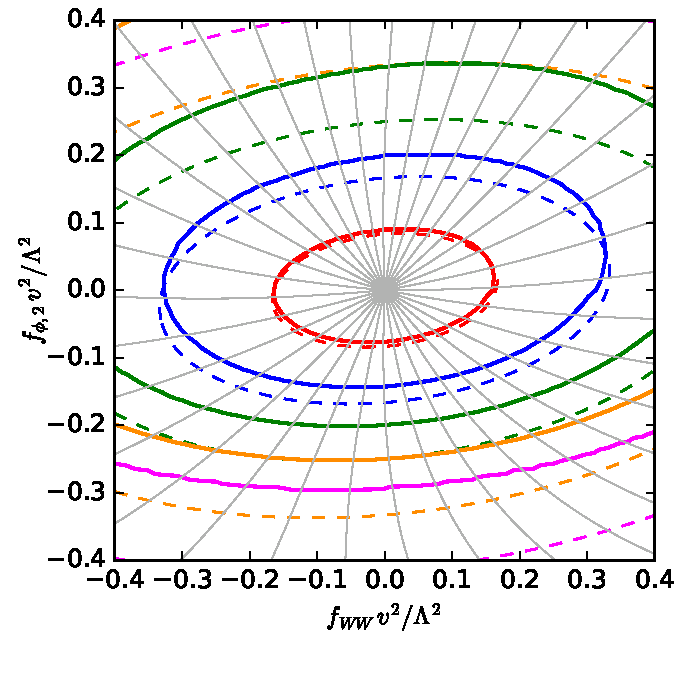
\includegraphics[width=0.33 \textwidth,clip,trim=0.3cm 0 0.05cm 0]{fig/information/wbf_4l_geometry_fphi2_fww}%
  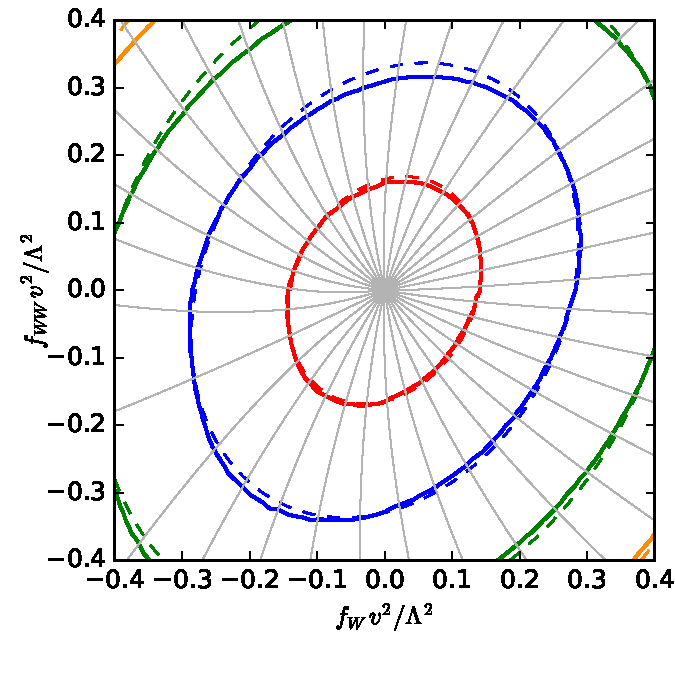
\includegraphics[width=0.33 \textwidth,clip,trim=0.3cm 0 0.05cm 0]{fig/information/wbf_4l_geometry_fww_fw}%
  \caption{Error ellipses defined by the Fisher information in the
    WBF $h \to 4\ell$ channel. We show contours of local distance
    $d_\text{local}(\boldtheta ; \boldzero)$ (dashed) and global
    distance $d(\boldtheta,\boldzero)$ (solid). The coloured contours
    indicate distances of $d = 1,2,3,4,5$. In grey we show example
    geodesics.  The $\theta_i$ not shown are set to zero.}
\label{fig:information_wbf_4l_geometry}
\end{figure}

The distribution of the differential information over phase space is
essentially identical to the results for the WBF $h \to \tau \tau$
mode given in
Figures~\ref{fig:information_wbf_tautau_differential_information_taus}
and \ref{fig:information_wbf_tautau_differential_information_jets},
with the obvious replacement of the reconstructed $\tau \tau$ system
by the $4 \ell$ system.



%%%%%%%%%%%%%%%%%%%%%%%%%%%%%%%%%%%%%%%%%%%%%%%%%%%%%%%%%%%%
\subsubsection*{Production vs decay kinematics}
%%%%%%%%%%%%%%%%%%%%%%%%%%%%%%%%%%%%%%%%%%%%%%%%%%%%%%%%%%%%

\begin{figure}
  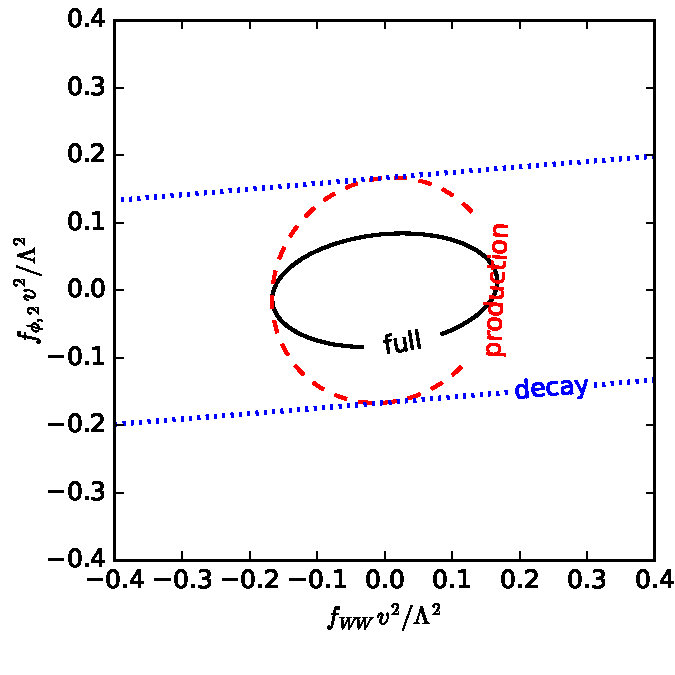
\includegraphics[width=0.49 \textwidth]{fig/information/wbf_4l_production_decay_fphi2_fww}
  \caption{Information in the WBF $h \to 4\ell$ channel from including
    dimension-six operators only in the production vertex (red), only in
    the decay vertex (blue), and in both vertices (black). The information is
    visualised as local contours
    $\dlocal(\boldtheta ; \boldzero) = 1$. The $\theta_i$ not shown
    are set to zero.}
\label{fig:information_wbf_4l_production_decay}
\end{figure}

The key question for the WBF $h\to 4\ell$ mode is how the rich decay
kinematics can improve the sensitivity to the dimension-six
operators. In \autoref{fig:information_wbf_4l_production_decay}, we
separately study the effects of the effective operators on the
production vertices only (fixing the decay vertex to the SM value) and
on the decay vertex (where the production is fixed to the SM
vertex). We find that only the sensitivity to $\ope{\phi,2}$ profits
from the decay vertex. Since this operator rescales all Higgs
couplings in the same way, this also applies to any other Higgs decay
mode. The sensitivity on the momentum-dependent operators $\ope{W}$,
$\ope{WW}$, $\ope{B}$, and $\ope{BB}$, on the other hand, comes almost
entirely from production-side effects.

This is not surprising: the momentum flow through the intermediate $W$
or $Z$ bosons can be very large at the LHC, enhancing production-side
effects by sizeable factors of $E^2 / \Lambda^2$. The momentum flow
through the decay vertices, on the other hand, is bounded by the Higgs
mass (neglecting off-shell Higgs decays), and $E^2 / \Lambda^2$ is
small. Our results show that this disadvantage is not compensated by
the complex $h \to 4\ell$ kinematics.



%%%%%%%%%%%%%%%%%%%%%%%%%%%%%%%%%%%%%%%%%%%%%%%%%%%%%%%%%%%%
\subsubsection*{Information in distributions}
%%%%%%%%%%%%%%%%%%%%%%%%%%%%%%%%%%%%%%%%%%%%%%%%%%%%%%%%%%%%

The question of production and decay effects can also be tackled by
comparing the information in different observables: the properties of
the tagging jets are linked to the production process, while the decay
products of the Higgs are mostly sensitive to the decay vertex. We
define the jet observables in complete analogy to the $\tau \tau$
channel in \autoref{sec:information_wbf_tautau}. These are complemented
by five observables characterising the decay
kinematics~\cite{Bolognesi:2012mm, Englert:2012xt}:
%
\begin{itemize}
\item the transverse momentum of the leading lepton, $p_{T,\ell_1}$;
  % 
\item the transverse momentum of the four-lepton system, $p_{T,4\ell}$, which is equal to the Higgs $p_T$;
  % 
\item the smaller invariant mass of the reconstructed $\ell^+ \ell^-$, $m_{Z_2}$;
  % 
\item the angle $\cos \theta_1 = \hat{p}_{\ell^-_1} \cdot \hat{p}_{Z_2}
  \Big|_{Z_1}$ with spatial unit vectors $\hat{p}$ defined in the $Z_1$ system;
  % 
\item analogously $\cos \theta_2$; and
  % 
\item the angle
  $\cos \Phi = ( \hat{p}_{\ell^-_1} \times \hat{p}_{\ell^+_1} )
  \cdot ( \hat{p}_{\ell^-_2} \times \hat{p}_{\ell^+_2} ) \Big|_{4\ell}$,
  defined in the $4\ell$ rest frame.
\end{itemize}
%
In all cases we use at least ten bins and include underflow and
overflow bins where applicable.

\begin{figure}
  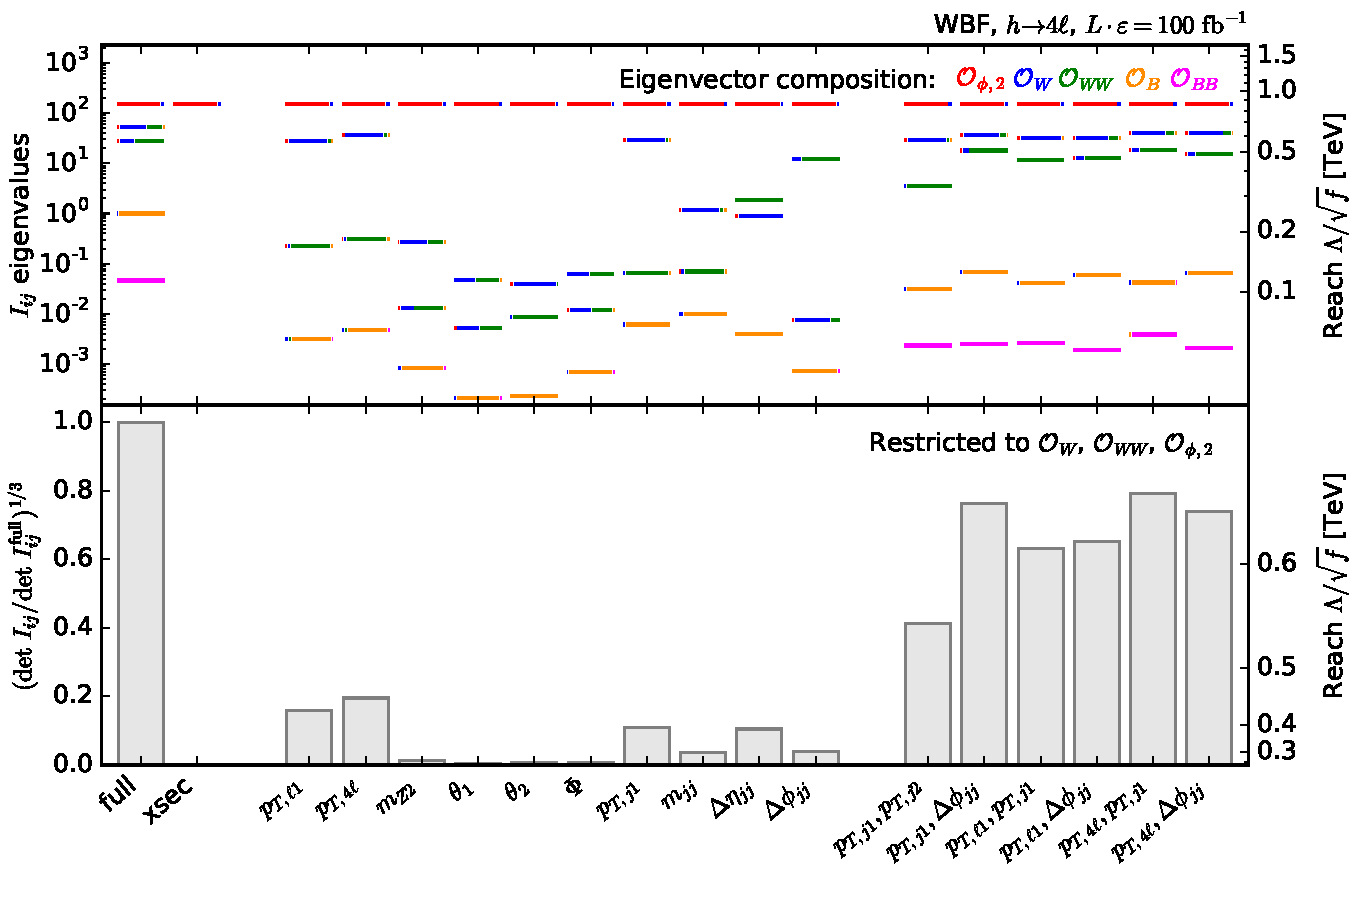
\includegraphics[width= \textwidth]{fig/information/wbf_4l_histos_comparison}
  \caption{Total Fisher information for the WBF $h \to 4 \ell$ channel
    (`full') compared to the information in several kinematic
    distributions. The top panel shows the eigenvalues, the colours
    denote the composition of the corresponding eigenvectors. The
    right axis translates the eigenvalues into a new physics reach for
    the corresponding combination of Wilson coefficients.  In the
    bottom panel we show the determinants of the Fisher information
    restricted to $\ope{\phi,2}$, $\ope{W}$, and $\ope{WW}$,
    normalised to the full information. Again, the right axis
    translates them into a new physics reach.}
\label{fig:information_wbf_4l_histograms_comparison}
\end{figure}

The comparison in
\autoref{fig:information_wbf_4l_histograms_comparison} reveals similar
patterns as the $\tau \tau$ mode. The key observables are again
transverse momenta and jet angular correlations. Without the
complication of removing backgrounds efficiently, the combined
analysis of these variables comes close to the maximum information: a
two-dimensional histogram of jet transverse momenta and
$\Delta \phi_{jj}$ probes new physics scales up to 650~GeV, while for
a fully differential analysis the maximum probed new physics scale is
close to 700~GeV. This difference roughly corresponds to 25\% more
data. The observables characterising the decay kinematics, in particular the
angular correlations, carry very little information, in agreement with
our previous results. This shows again how much the sensitivity of the
decay vertices to dimension-six operators is limited by the
restriction of the momentum flow through the decay vertex to the Higgs
mass. 

To overcome this disadvantage, momentum-dependent signatures in Higgs
decays require a large production cross section. Gluon-fusion
production with $h \to 4\ell$ channel has a rate that is approximately
13 times larger than the WBF process studied
here~\cite{deFlorian:2016spz}. Since the decay kinematics is the same
as in the process studied here and the Fisher information scales
linearly with the number of events, we can provide a rough estimate of
the information in this process by scaling the decay-only Fisher
information with this factor 13. We find that even with the increased
rate from production in gluon fusion, the $h \to 4 \ell$ is not as
sensitive to Higgs-gauge operators as the WBF production process. Of
course, this simple estimate ignores the differences in the production
kinematics.



% %%%%%%%%%%%%%%%%%%%%%%%%%%%%%%%%%%%%%%%%%%%%%%%%%%%%%%%%%%%%
% \subsubsection*{Summary}
% %%%%%%%%%%%%%%%%%%%%%%%%%%%%%%%%%%%%%%%%%%%%%%%%%%%%%%%%%%%%

% Higgs production in weak boson fusion with a $h \to 4 \ell$ decay is a
% $2 \to 6$ process with a clean signature and very rich kinematics. We
% use it to compare the sensitivity to dimension-six physics in the
% decay and production vertices within the same process. Our results are
% unambiguous: the diverse decay kinematics is much less sensitive to
% momentum-dependent operators than the production-side probes provided
% by the tagging jets. This reflects the $E^2/\Lambda^2$ dependency of
% such dimension-six effects, which can be large in the production
% vertex, while the momentum flow through the decay vertex is limited to
% the Higgs mass.

% The clean $4\ell$ final state means that the Higgs can be
% reconstructed nearly free from background contributions, and a simple
% analysis of jet transverse momenta and angular correlations can access
% most of the information in the process.

% This is not accidental: the reason behind this role of the momentum
% dependence is that for all operators shown in
% \autoref{eq:information_wilson_space_wbf} with the exception of
% $\ope{\phi,2}$, gauge invariance forces us to include the field
% strength tensor instead of the gauge boson field, automatically
% introducing a momentum dependence.



%%%%%%%%%%%%%%%%%%%%%%%%%%%%%%%%%%%%%%%%%%%%%%%%%%%%%%%%%%%%
\subsection{Higgs plus single top}
\label{sec:information_th}
%%%%%%%%%%%%%%%%%%%%%%%%%%%%%%%%%%%%%%%%%%%%%%%%%%%%%%%%%%%%

Our final example process
% for $CP$-even dimension-six operators
is Higgs production with a single top in the $t$ channel. We focus on
the $h \to \gamma \gamma$ mode and a hadronic top decay $t \to b
jj$.
As shown in \autoref{fig:information_th_diag}, diagrams where the
Higgs is radiated off a $W$ boson interfere destructively with
diagrams with a top-Higgs coupling, making this channel a direct probe
of the sign of the top Yukawa coupling~\cite{Maltoni:2001hu}. Our
analysis focuses on the question which of the phase-space
distributions provide access to this interesting amplitude
structure. We stick to a parton-level analysis at leading order in the
five-flavor scheme. For our toy example we include only one of the
dominant backgrounds, single top production with two photons, and in
particular ignore the multi-jet background. The subleading
$t\bar{t} \, \gamma\gamma$ background populates qualitatively
different phase-space regions from the single-top signal and can be
suppressed with an appropriate event selection~\cite{Kling:2012up}.

\begin{figure}
  \fmfframe(0,15)(15,15){ %(L,T) (R,B)
    \begin{fmfgraph*}(150,70)
      \feynmansetup 
      \fmfleft{i2,i1}
      \fmfright{o6,o5,o4,blind3,o3,o2,blind3,blind1,blind2,o1}
      \fmflabel{\small $q$}{i1}
      \fmflabel{\small $b$}{i2}
      \fmflabel{\small $q$}{o1}
      \fmflabel{\small $\gamma$}{o2}
      \fmflabel{\small $\gamma$}{o3}
      \fmflabel{\small $q$}{o4}
      \fmflabel{\small $q$}{o5}
      \fmflabel{\small $b$}{o6}
      %
      % Upper quark line
      \fmf{fermion,tension=6}{i1,v1}
      \fmf{fermion,tension=1.7}{v1,o1}
      %
      % Lower quark line
      \fmf{fermion,tension=6}{i2,v3}
      \fmf{fermion,label=\small $t$,label.side=right,tension=3}{v3,v5}
      \fmf{fermion,tension=3.5}{v5,o6}
      %
      % W exchange 
      \fmf{wiggly,label=\small $W$,label.side=right}{v1,v2}
      \fmf{wiggly,label=\small $W$,label.side=right}{v2,v3}
      %
      % Higgs 
      \fmf{dashes,label=\small $h$,label.side=left,tension=0.2}{v2,v4}
      \fmf{wiggly,tension=0.35}{o2,v4,o3}
      %
      % Top decay 
      \fmf{wiggly,label=\small $W$,label.side=left,tension=0.7}{v5,v6}
      \fmf{fermion,tension=0.5}{o4,v6,o5}
      \fmfv{decoration.shape=circle,foreground=(0.8,, 0.0,, 0.0),decoration.size=5}{v2,v4}
    \end{fmfgraph*}
  }
  \hspace{1cm}
  \fmfframe(0,15)(15,15){ %(L,T) (R,B)
    \begin{fmfgraph*}(150,70)
      \feynmansetup
      \fmfleft{i2,i1}
      \fmfright{o6,o5,o4,blind2,o3,o2,blind1,o1}
      \fmflabel{\small $q$}{i1}
      \fmflabel{\small $b$}{i2}
      \fmflabel{\small $q$}{o1}
      \fmflabel{\small $\gamma$}{o2}
      \fmflabel{\small $\gamma$}{o3}
      \fmflabel{\small $q$}{o4}
      \fmflabel{\small $q$}{o5}
      \fmflabel{\small $b$}{o6}
      %
      % Upper quark line
      \fmf{fermion,tension=6}{i1,v1}
      \fmf{fermion,tension=1.7}{v1,o1}
      %
      % Lower quark line
      \fmf{fermion,tension=3}{i2,v3}
      \fmf{fermion,label=\small $t$,label.side=right,tension=2}{v3,v2}
      \fmf{fermion,label=\small $t$,label.side=right,tension=1.5}{v2,v5}
      \fmf{fermion,tension=1.5}{v5,o6}
      %
      % W exchange 
      \fmf{wiggly,label=\small $W$,label.side=right}{v1,v3}
      %
      % Higgs 
      \fmf{dashes,label=\small $h$,label.side=left,tension=0.5}{v2,v4}
      \fmf{wiggly,tension=0.6}{o2,v4,o3}
      %
      % Top decay 
      \fmf{wiggly,label=\small $W$,label.side=left,tension=0.6}{v5,v6}
      \fmf{fermion,tension=0.4}{o4,v6,o5}
      %
      \fmfv{decoration.shape=circle,foreground=(0.8,, 0.0,, 0.0),decoration.size=5}{v2,v4}
    \end{fmfgraph*}
  }
  \caption{Feynman diagrams for Higgs production with a single top
    quark with $h \to \gamma \gamma$ and a hadronic top decay. The red
    dots show the Higgs interactions modified by the dimension-six
    operators considered in our analysis.}
  \label{fig:information_th_diag}
\end{figure}

To simulate the experimental mass resolution, we smear the
$m_{\gamma \gamma}$ distribution of the signal process with the
smearing function of Reference~\cite{Kling:2016lay} described in
\autoref{sec:appendix_information_smearing}. We do not include any
other detector effects. Our basic event selection requires
%
\begin{align}
  p_{T,j} &> 20 \ \gev  & 
  |\eta_{j}| &< 5.0  & 
  \Delta R_{jj} &> 0.4  & 
  152 \ \gev &<m_{bjj} < 192 \ \gev \notag \\ 
  p_{T,\gamma} &> 10 \ \gev  & 
  |\eta_{\gamma}| &< 2.5  &  
  \Delta R_{\gamma j} , \Delta R_{\gamma \gamma} &> 0.4  & 
  120 \ \gev &<m_{\gamma \gamma} < 130 \ \gev \,,
  \label{eq:information_th_acceptance_cuts}
\end{align}
%
after which the SM signal of $0.10~\fb$ faces a background of $0.22~\fb$. We
calculate the Fisher information for $pp$ collisions at
$\sqrt{s} = 13~\tev$ with a large amount of collected data,
%
\begin{equation}
  L \cdot \varepsilon = 300~\ifb \,.
\end{equation}
%
Again, $\varepsilon$ denotes the combined particle identification and
trigger efficiencies. This is equivalent to 30 expected signal events
and 66 expected background events.

Out of the $CP$-even dimension-six operators discussed in
\autoref{sec:foundations_heft_operators}, $\ope{W}$ and $\ope{WW}$
modify the Higgs-$W$ coupling structure, while $\ope{t}$ changes the
value of the Higgs-top coupling. $\ope{\phi,2}$ rescales both
contributions universally. While all these operators affect the
$h\to \gamma \gamma$ decay as well, the largest effect is expected
from $\ope{WW}$, which contributes to this coupling at tree level and
can easily compete with the loop-suppressed SM term. Since we are
mainly interested in the production kinematics, we neglect the
subleading effects from $\ope{W}$ and $\ope{t}$ on the Higgs-photon
coupling. Our model space is therefore parametrised by the
dimensionless parameters
%
\begin{equation}
  \boldtheta = \frac {v^2} {\Lambda^2}  \fourvec {f_{\phi,2}} {f_W} {f_{WW}} {f_{t}} \,.
\end{equation}

As in the previous processes, we focus on the Fisher information in
the vicinity of the SM, $\boldtheta = \boldzero$, and in the
two-dimensional planes in the parameter space where all but two
operators are set to zero. Using the setup described in
\autoref{sec:information_algorithm}, we calculate the Fisher
information for approximately 2500 parameter points.



%%%%%%%%%%%%%%%%%%%%%%%%%%%%%%%%%%%%%%%%%%%%%%%%%%%%%%%%%%%%
\subsubsection{Total Fisher information}
%%%%%%%%%%%%%%%%%%%%%%%%%%%%%%%%%%%%%%%%%%%%%%%%%%%%%%%%%%%%

Using our setup described in \autoref{sec:information_algorithm}, we
calculate the total Fisher information at the SM to be
%
\begin{equation}
  I_{ij} (\boldzero) =
\begin{pmatrix*}[r]
  80.1 & -18.7 & -957.0 & 13.2 \\
  -18.7 & 32.6 & 221.7 & 27.0 \\
  -957.0 & 221.7 & 11446.1 & -146.0 \\
  13.2 & 27.0 & -146.0 & 150.3
\end{pmatrix*} \,.
\end{equation}
%
Composing this into eigenvectors and eigenvalues (and the
corresponding new physics reach, see
\autoref{eq:information_new_physics_reach}), we find
%
\begingroup%
\allowdisplaybreaks%
\begin{align}
  \boldtheta_1 &= \fourvecr {0.08} {-0.02} {-1.00} {0.01} \,:
  & I_1 &= 11532
  &&\leftrightarrow
  & \left( \frac {\Lambda} {\sqrt{f}} \right)_1 &= 2550~\gev \,, \notag \\
  %
  \boldtheta_2 &= \fourvecr {0.00} {-0.23} {-0.01} {-0.97} \,:
  & I_2 &= 155
  &&\leftrightarrow
  & \left( \frac {\Lambda} {\sqrt{f}} \right)_2 &= 868~\gev \,, \notag \\
  %
  \boldtheta_3 &= \fourvecr {-0.02} {0.97} {-0.02} {-0.23}\,:
  & I_3 &= 21.3
  &&\leftrightarrow
  & \left( \frac {\Lambda} {\sqrt{f}} \right)_3 &= 528~\gev \,, \notag \\
  %
  \boldtheta_4 &= \fourvecr {1.00} {0.02} {0.08} {-0.01}\,:
  & I_4 &= 0.1
  &&\leftrightarrow
  & \left( \frac {\Lambda} {\sqrt{f}} \right)_4 &= 138~\gev \,. 
\end{align}%
\endgroup
%
The large sensitivity to $\ope{WW}$ comes from the large effect of
this operator on the $h \to \gamma \gamma$ decay in addition to
production effects, which will already be tightly constrained once a
$th$ measurement is feasible. The orthogonal direction in the
$\ope{\phi,2}$-$\ope{WW}$ plane is for all practical purposes
blind. Even with the large amount of integrated luminosity that this
calculation is based on, the sensitivity to $\ope{W}$ and $\ope{t}$ is
limited, with some mixing between the two operators. 

\thpyramid{th_global}{fig:information_th_global_distances} {Error
  ellipses defined by the Fisher information in Higgs plus single top
  production. We show global distances from the SM
  $d(\boldtheta,\boldzero)$, where in each panel the $\theta_i$ not
  shown are set to zero. The white contours show distances of
  $d=1, 2, \dots , 5$.}

Going beyond the local information geometry, we calculate global
information distances in the model space and show them in
\autoref{fig:information_th_global_distances}. These results confirm the
small sensitivity of this process to all operators except
$\ope{WW}$. Local and global distances are compared in
\autoref{fig:information_th_geometry}.  Large differences are visible
at the $d = 2$ level, implying that a measurement of this channel will
always be sensitive to the squared dimension-six terms.

\begin{figure}
  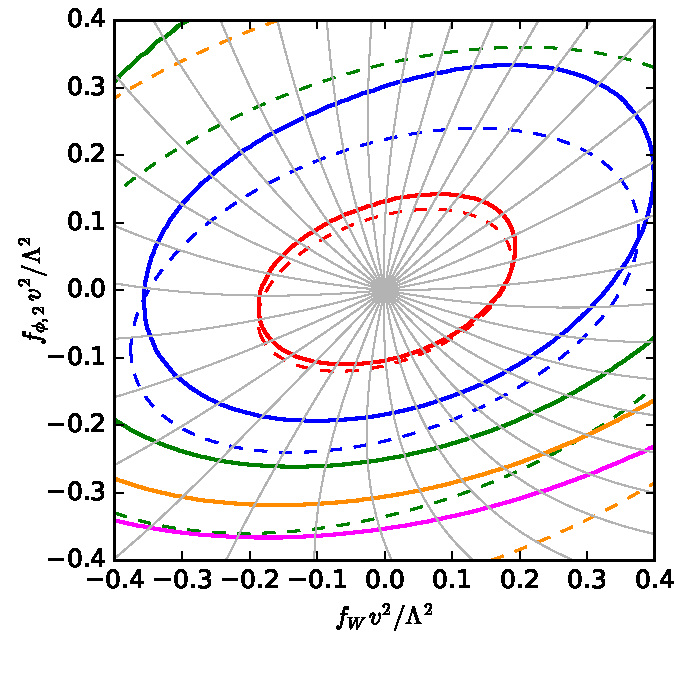
\includegraphics[width=0.33 \textwidth,clip,trim=0.3cm 0 0.05cm 0]{fig/information/th_geometry_fphi2_fw}%
  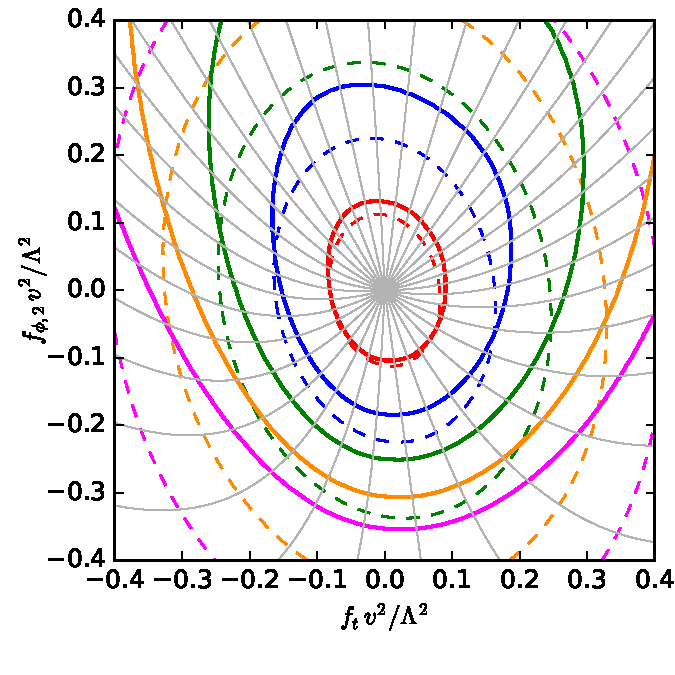
\includegraphics[width=0.33 \textwidth,clip,trim=0.3cm 0 0.05cm 0]{fig/information/th_geometry_fphi2_ft}%
  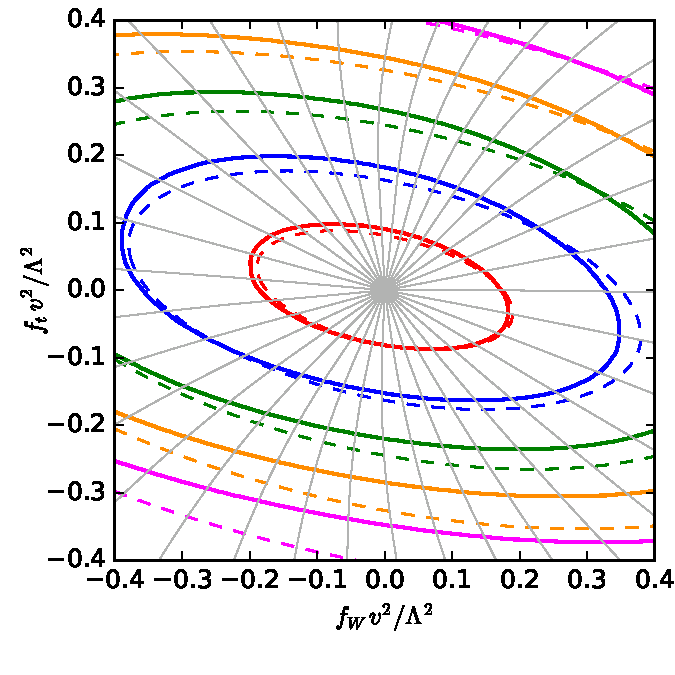
\includegraphics[width=0.33 \textwidth,clip,trim=0.3cm 0 0.05cm 0]{fig/information/th_geometry_ft_fw}%
  \caption{Error ellipses defined by the Fisher information in Higgs
    plus single top production. We show contours of local distance
    $d_\text{local}(\boldtheta ; \boldzero)$ (dashed) and global
    distance $d(\boldtheta,\boldzero)$ (solid).  The coloured contours
    indicate distances of $d = 1,2,3,4,5$. In grey we show example
    geodesics. The $\theta_i$ not shown are set to zero. }
\label{fig:information_th_geometry}
\end{figure}



%%%%%%%%%%%%%%%%%%%%%%%%%%%%%%%%%%%%%%%%%%%%%%%%%%%%%%%%%%%%
\subsubsection{Differential information}
%%%%%%%%%%%%%%%%%%%%%%%%%%%%%%%%%%%%%%%%%%%%%%%%%%%%%%%%%%%%

\begin{figure}
  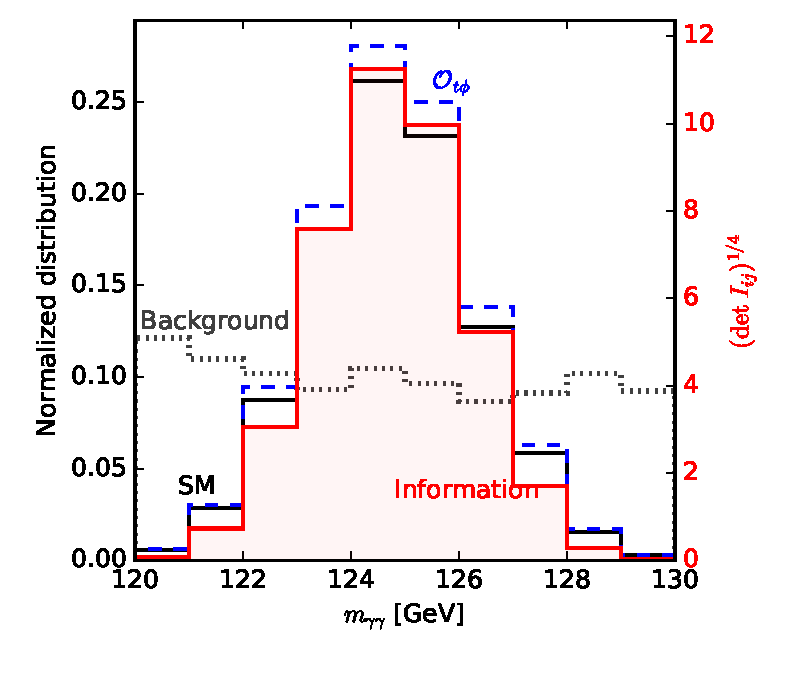
\includegraphics[width=0.49 \textwidth]{fig/information/th_information_over_maa}%
  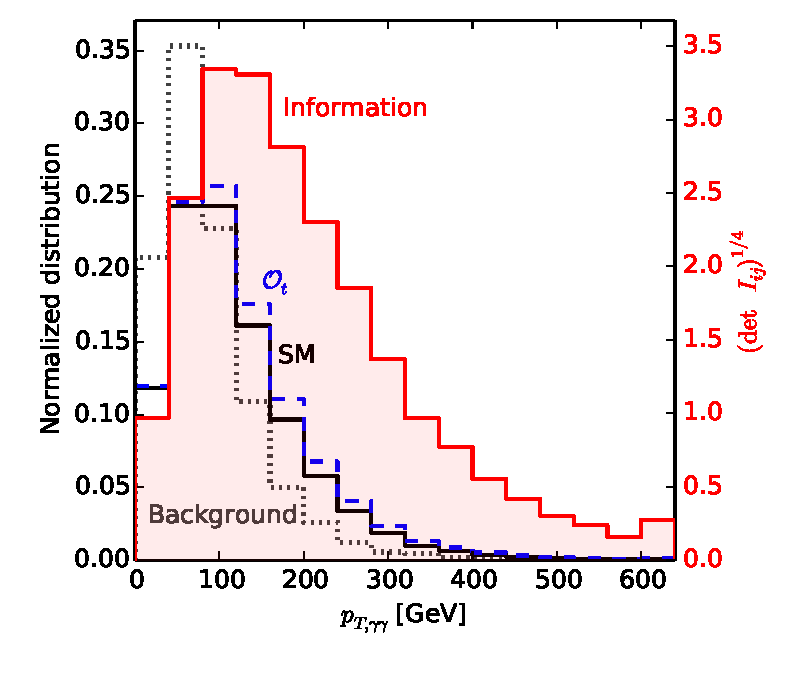
\includegraphics[width=0.49 \textwidth]{fig/information/th_information_over_ptaa}%
  \caption{Distribution of the differential SM Fisher information in
    the Higgs plus single top channel (shaded red) with respect to the
    mass (left) and transverse momentum (right) of the diphoton
    system. We also show the normalised SM signal (solid black) and
    the single-top background (dotted grey) rates. The dashed blue
    line shows the effect of $f_{t} \, v^2 / \Lambda^2 = 0.2$. In the
    right panel, the last bin is an overflow bin.}
  \label{fig:information_th_differential_information_photons}
\end{figure}

In Figures~\ref{fig:information_th_differential_information_photons}
and \ref{fig:information_th_differential_information_jets} we show the
distribution of this information over phase space. As expected, the
discrimination power is concentrated in the
$m_{\gamma \gamma} \sim m_H$ peak and in the high-energy tails of the
transverse momenta of jets or photons. Studying angular correlations
between the diphoton system and the top decay products, we find that the
region $\Delta \eta_{ \gamma \gamma, bjj} \lesssim 3$ contains a lot
of information.

\begin{figure}
  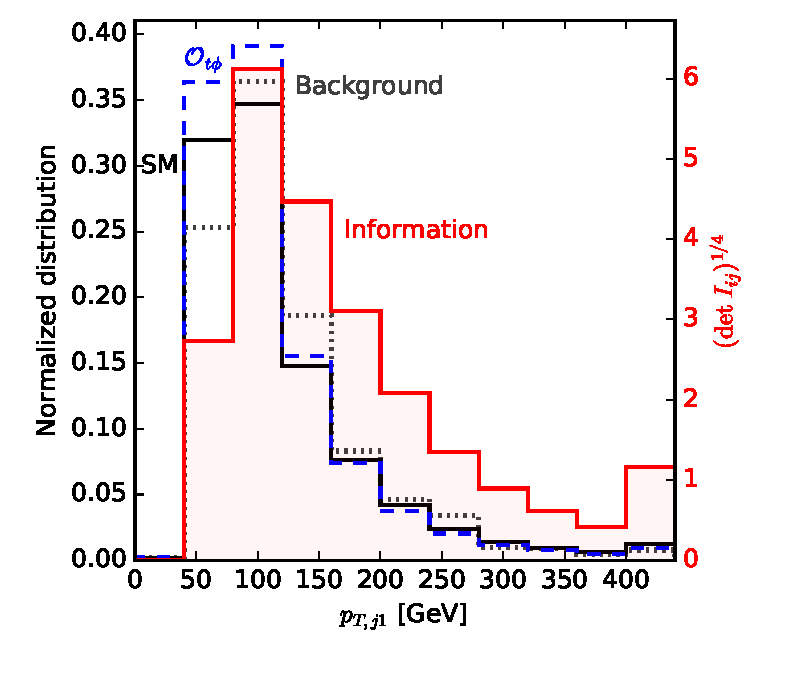
\includegraphics[width=0.49 \textwidth]{fig/information/th_information_over_ptj}%
  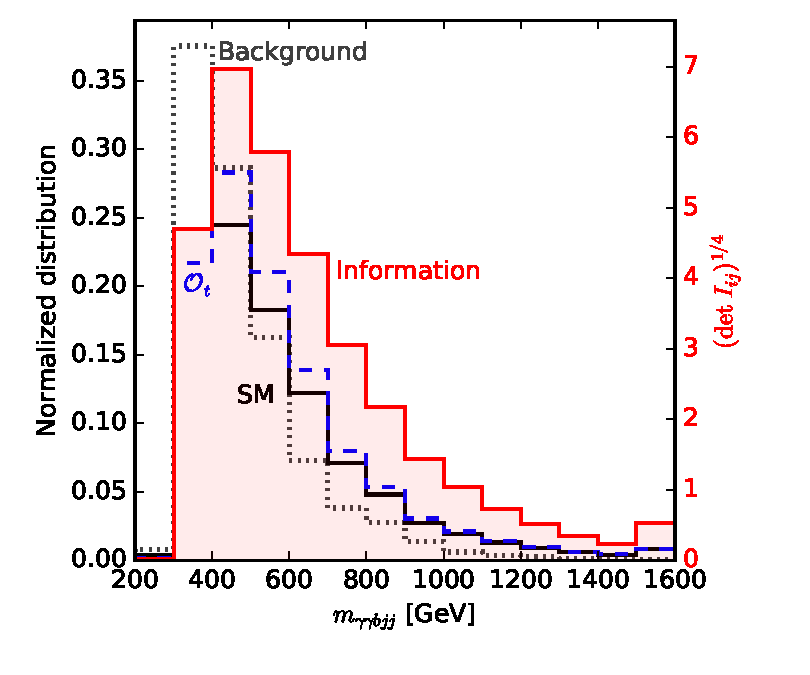
\includegraphics[width=0.49 \textwidth]{fig/information/th_information_over_maabjj}\\%
  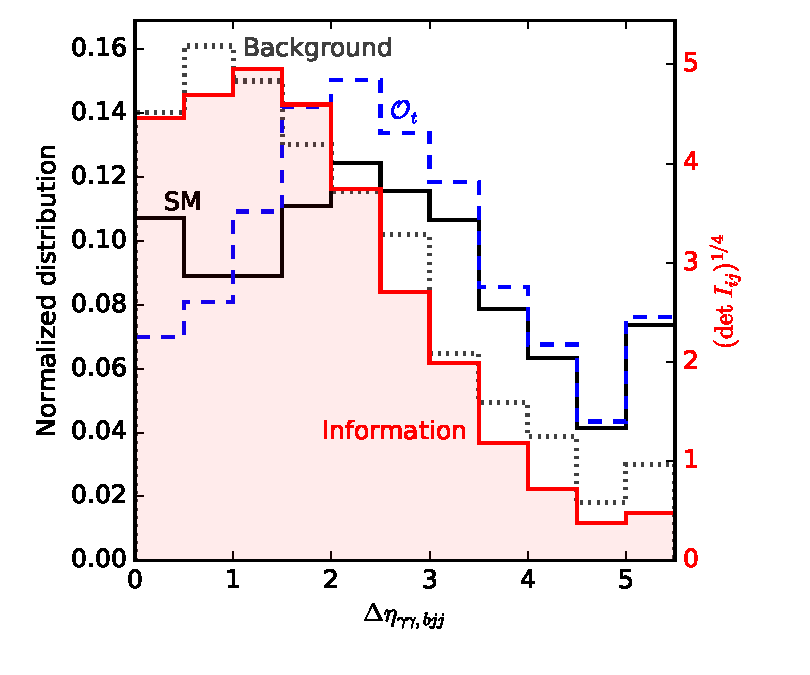
\includegraphics[width=0.49 \textwidth]{fig/information/th_information_over_deltaeta}%
  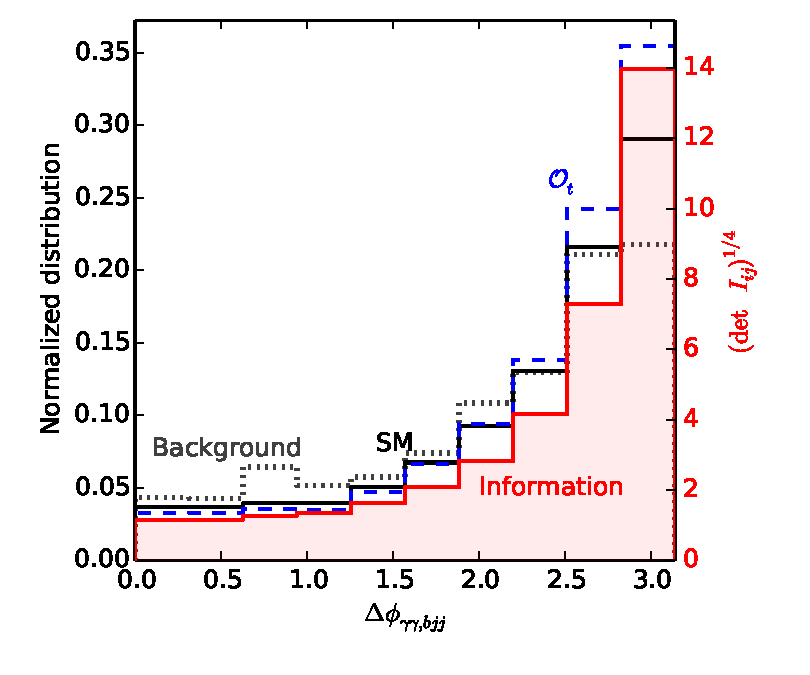
\includegraphics[width=0.49 \textwidth]{fig/information/th_information_over_deltaphi}%
  \caption{Distribution of the differential SM Fisher information in
    the Higgs plus single top channel (shaded red) with respect to the
    transverse momentum of the leading jet (top left), the invariant
    mass of the whole $th$ system (top right), and the differences in
    pseudorapidity and azimuthal angle between the diphoton system and
    the top decay products (bottom). We also show the normalised SM
    signal (solid black) and the single-top background (dotted grey)
    rates. The dashed blue line shows the effect of
    $f_{t} \, v^2 / \Lambda^2 = 0.2$. The last bins are overflow bins
    where applicable.}
  \label{fig:information_th_differential_information_jets}
\end{figure}




%%%%%%%%%%%%%%%%%%%%%%%%%%%%%%%%%%%%%%%%%%%%%%%%%%%%%%%%%%%%
\subsubsection*{Information in distributions}
%%%%%%%%%%%%%%%%%%%%%%%%%%%%%%%%%%%%%%%%%%%%%%%%%%%%%%%%%%%%

The next question is again how much of this maximal information is contained in various kinematic distributions. A histogram-based analysis requires a reasonable signal-to-background ratio, so we require
%
\begin{equation}
  p_{T,j_1} > 50~\gev \qquad 
  p_{T,\gamma} > 50,~30~\gev \qquad
  122~\gev < m_{\gamma \gamma} < 128~\gev \,.
  \label{eq:information_th_cuts}
\end{equation}
%
This reduces the single-top background to the level of the
signal. Based on this selection, we analyse the information in the
following distributions:
%
\begin{itemize}
\item the transverse momentum of the leading photon, $p_{T,\gamma_1}$,
  with bin size 25~GeV up to 400~GeV and an overflow bin;
%
\item the invariant mass of the diphoton system, $m_{\gamma\gamma}$,
  with bin size 1~GeV in the allowed range of $123~...~127~\gev$;
%
\item the transverse momentum of the diphoton system,
  $p_{T,\gamma \gamma}$ with bin size 40~GeV up to 600~GeV and an
  overflow bin;
%
\item the separation in azimuthal angle between the two photons,
  $\Delta \phi_{\gamma \gamma}$, with bin size $\pi/10$;
%
\item the transverse momentum of the leading light (\ie non-$b$) jet,
  $p_{T,j_1}$, with bin size 40~GeV up to 400~GeV and an overflow bin;
%
\item the transverse momentum of the $b$ jet, $p_{T,b}$, with bin size
  40~GeV up to 400~GeV and an overflow bin;
%
\item the transverse momentum of the reconstructed $t$ momentum,
  $p_{T,bjj}$, with bin size 40~GeV up to 600~GeV and an overflow bin;
%
\item the separation in azimuthal angle between the diphoton system
  and the $b$ jet, $\Delta \phi_{\gamma \gamma, b}$, with bin size
  $\pi / 10$;
%
\item the separation in pseudorapidity between the diphoton system and
  the $b$ jet, $\Delta \eta_{\gamma\gamma, b}$, with bin size $0.5$ up
  to $5.0$ and an overflow bin;
%
\item the invariant mass of the full $th$ system, $m_{\gamma \gamma bjj}$, with bin size 100~GeV up to 1500~GeV and an
  overflow bin;
%
\item the transverse momentum of the full $th$ system,
  $p_{T,\gamma \gamma bjj}$ with bin size 40~GeV up to 400~GeV and an
  overflow bin;
%
\item the separation in azimuthal angle between the diphoton system and
  the reconstructed $t$ momentum, $\Delta \phi_{\gamma \gamma, bjj}$, with bin size $\pi / 10$; and
%
\item the separation in pseudorapidity between the diphoton system and
  the reconstructed $t$ momentum, $\Delta \eta_{\gamma\gamma, bjj}$,
  with bin size $0.5$ up to $5.0$ and an overflow bin.
\end{itemize} 

\begin{figure}
  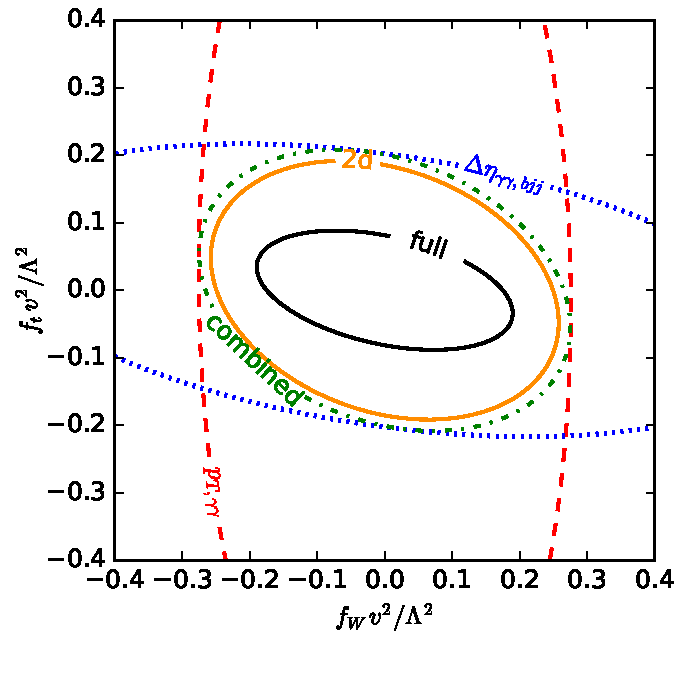
\includegraphics[width=0.49 \textwidth]{fig/information/th_histos_contours}
  \caption{Information from histograms compared to the full
    information (black), shown as contours
    $\dlocal(\boldtheta ; \boldzero) = 1$. We include
    $p_{T,\gamma \gamma}$, $\Delta \eta_{\gamma\gamma, bjj}$, their naive combination assuming
    no mutual information, and their two-dimensional histogram. The
    $\theta_i$ not shown are set to zero.}
  \label{fig:information_th_histograms_contours}
\end{figure}

As in the WBF case, different observables probe different Wilson
operators. In \autoref{fig:information_wbf_tautau_histograms_contours}
we demonstrate that the diphoton transverse momentum constrains mostly
the $\ope{W}$ direction, while the rapidity separation between the
Higgs and top systems is more sensitive to $\ope{t}$.

\begin{figure}
  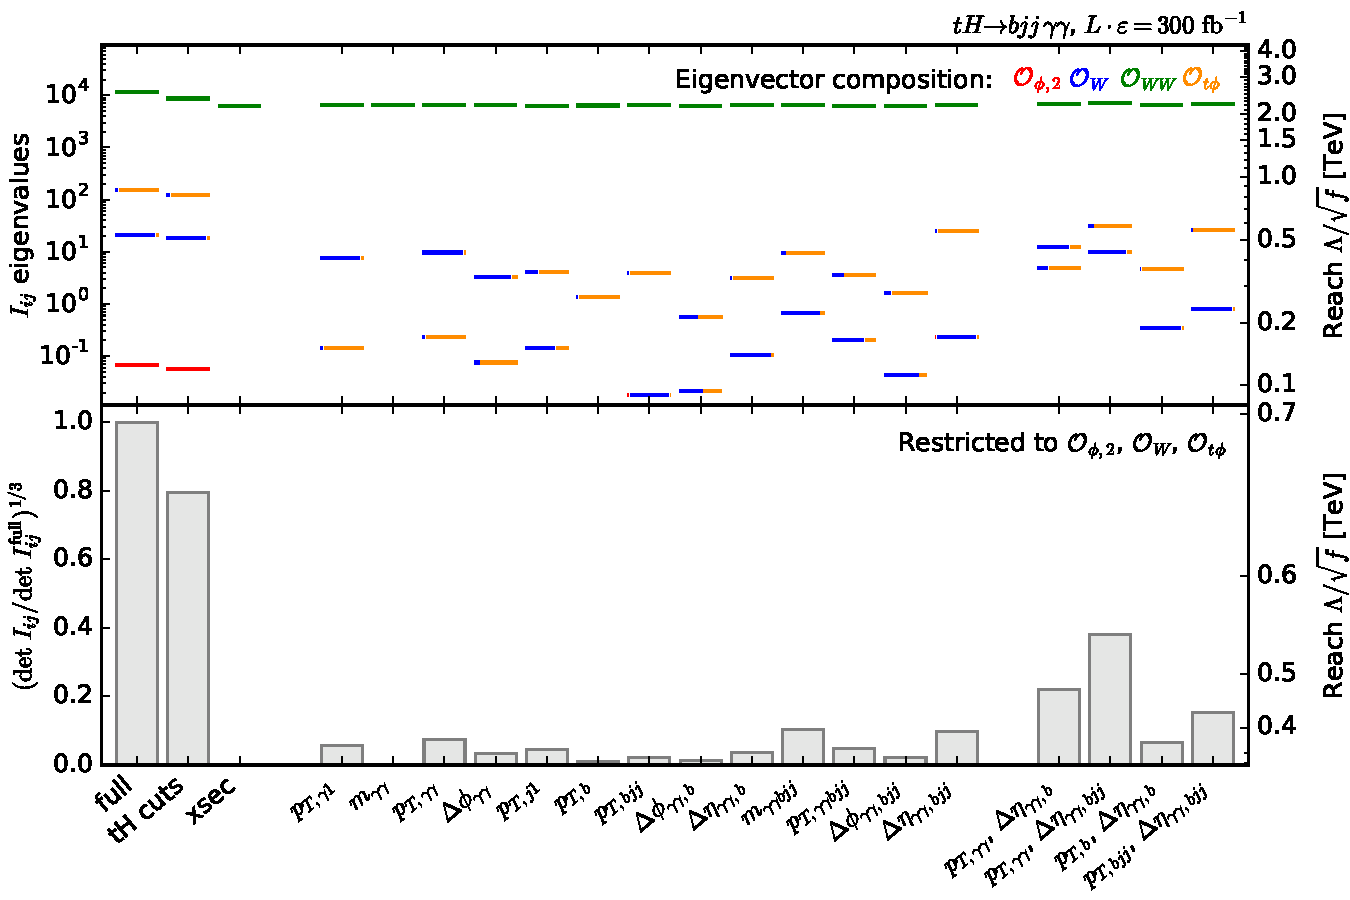
\includegraphics[width= \textwidth]{fig/information/th_histos_comparison}
  \caption{Total Fisher information for the Higgs plus single top
    channel (`full'), Fisher information after the $th$ cuts in
    \autoref{eq:information_th_cuts}, and the information in several
    distributions after this selection.  The top panel shows the
    eigenvalues, the colours denote the composition of the
    corresponding eigenvectors. The right axis translates the
    eigenvalues into a new physics reach for the corresponding
    combination of Wilson coefficients.  In the bottom panel we show
    the determinants of the Fisher information restricted to
    $\ope{\phi,2}$, $\ope{W}$, and $\ope{t}$, normalised to the full
    information. Again, the right axis translates them into a new
    physics reach.}
\label{fig:information_th_histograms_comparison}
\end{figure}

In \autoref{fig:information_th_histograms_comparison} we compare the
eigenvalues, eigenvectors, and determinants of the information
matrices in all of the above distributions, in analogy to
\autoref{fig:information_wbf_tautau_histograms_comparison}. We confirm
that the photon observables mostly probe changes in the Higgs-gauge
coupling from $\ope{W}$, while a rescaled top Yukawa will be visible
in the properties of the top decay products. Distributions of the
properties of the $b$ jet consistently contain significantly less
information than the corresponding distributions for the reconstructed
top system. The rapidity difference between the $\gamma \gamma$ system
and the reconstructed top provides a particularly good probe of this
operator. Combining this variable with the transverse momentum of the
$\gamma \gamma$ system, we can probe new physics scales in the
$\ope{\phi,2}$-$\ope{W}$-$\ope{t}$ space of around
$\Lambda / \sqrt{f} \sim 550~\gev$, compared to $700~\gev$ based on
the full high-dimensional kinematics. This corresponds to almost three
times as much data. Of course, the histogram-based analysis would profit
from an optimisation of the selection cuts in
\autoref{eq:information_th_cuts}, which goes beyond the scope of this
demonstration.



%%%%%%%%%%%%%%%%%%%%%%%%%%%%%%%%%%%%%%%%%%%%%%%%%%%%%%%%%%%%
% \subsubsection{Summary}
%%%%%%%%%%%%%%%%%%%%%%%%%%%%%%%%%%%%%%%%%%%%%%%%%%%%%%%%%%%%

% Higgs production in association with a single top has an interesting
% amplitude structure where diagrams with Higgs-gauge interactions
% interfere destructively with diagrams depending on the top Yukawa
% coupling. Small changes to these interactions can in principle change
% the rate and kinematics drastically. We find that kinematic properties
% of the Higgs decay products and observables related to the top system
% provide orthogonal information on the theory space; in particular the
% diphoton transverse momentum as well as the rapidity separation of the
% $\gamma \gamma$ and the $bjj$ system provide useful information.

% Unfortunately, the tiny cross section of this process strongly limits
% the constraining power on dimension-six operators. Even with
% $300~\ifb$ of data, assuming perfect efficiencies, these distributions
% are only sensitive to new physics scales around $550~\gev$, while an
% optical multivariate analysis might be able to probe scales up to
% $700~\gev$ according to the Cram\'er-Rao bound.




% %%%%%%%%%%%%%%%%%%%%%%%%%%%%%%%%%%%%%%%%%%%%%%%%%%%%%%%%%%%%
% \section{$CP$ violation in the Higgs sector}
% \label{sec:information_application_odd}
% %%%%%%%%%%%%%%%%%%%%%%%%%%%%%%%%%%%%%%%%%%%%%%%%%%%%%%%%%%%%

% \comment{Wait for Felix\dots}



%%%%%%%%%%%%%%%%%%%%%%%%%%%%%%%%%%%%%%%%%%%%%%%%%%%%%%%%%%%%
\section{Extensions}
\label{sec:information_extensions}
%%%%%%%%%%%%%%%%%%%%%%%%%%%%%%%%%%%%%%%%%%%%%%%%%%%%%%%%%%%%

The applications of information geometry in the previous sections were
based on a number of simplifying assumptions. Most importantly, we
only considered statistical sources of uncertainty, and neglected
systematic and theory uncertainties on the signal and background
predictions. In \autoref{sec:information_systematics} we show how such
effects can be added to our approach.

\autoref{sec:information_comparison} finally compares the Fisher
information to two other statistical tools, the well-known
log-likelihood ratio and the ambient information geometry.



%%%%%%%%%%%%%%%%%%%%%%%%%%%%%%%%%%%%%%%%%%%%%%%%%%%%%%%%%%%%
\subsection{Systematic uncertainties}
\label{sec:information_systematics}
%%%%%%%%%%%%%%%%%%%%%%%%%%%%%%%%%%%%%%%%%%%%%%%%%%%%%%%%%%%%

The precision of most Higgs measurements at the LHC will ultimately be
limited by systematic and theory
uncertainties~\cite{deFlorian:2016spz, Khachatryan:2016vau}. The
expected differential rates of cross sections of signal and
backgrounds are then not exactly known, but depend on unknown nuisance
parameters $\boldnu$. In \autoref{sec:information_nuisance} we showed
how these can be incorporated in our approach, and defined a profiled
Fisher information that conservatively includes systematic
uncertainties. 

\begin{figure}
  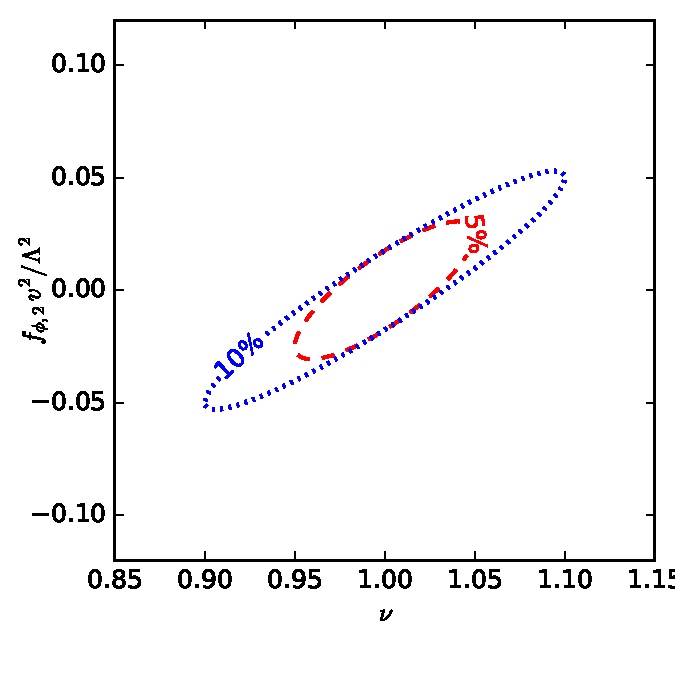
\includegraphics[width=0.49 \textwidth]{fig/information/wbf_tautau_systematics_nuisance.pdf}%
  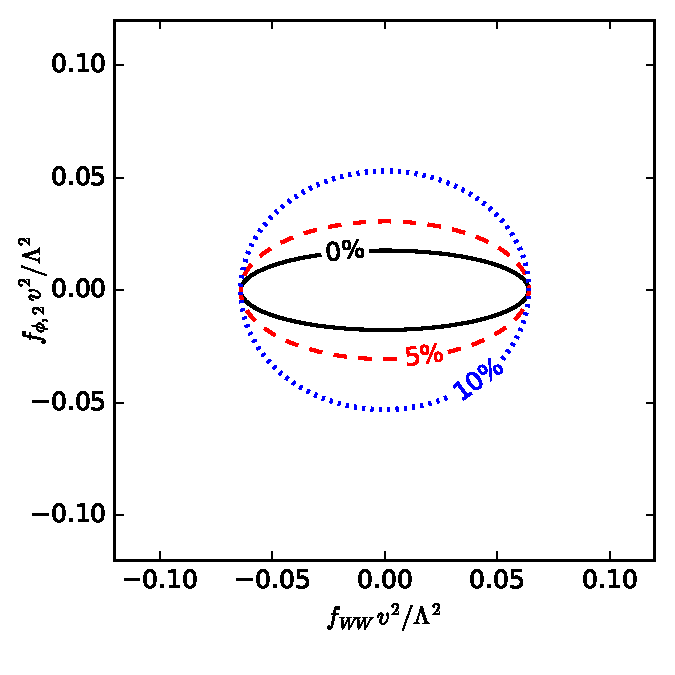
\includegraphics[width=0.49 \textwidth]{fig/information/wbf_tautau_systematics_profiled.pdf}%
  \caption{Effects of Gaussian uncertainties of $5\%$ and $10\%$ on
    the total signal rate. In the left panel we show the expected
    error ellipse $\dlocal( (\theta,\nu) ; \boldzero) = 1$ in the
    plane spanned by a physical parameter $\theta$ and the nuisance
    parameter $\nu$ rescaling the signal rate. In the right panel we
    show the error ellipses in the $\ope{W}$-$\ope{\phi,2}$ plane
    after profiling over this systematic uncertainty.}
  \label{fig:information_wbf_tautau_systematics}
\end{figure}

We now demonstrate this tool for the information on $CP$-even
dimension-six operators in WBF Higgs production in the $\tau \tau$
mode. Our setup is the same as in \autoref{sec:information_wbf_tautau},
except that we assign a $5\%$ or $10\%$ Gaussian uncertainty on the
overall signal rate, representing for instance missing higher orders,
pdf or efficiency uncertainties. After profiling over this nuisance
parameter, the information in the total rate is significantly reduced,
which mostly limits the precision in the $\ope{\phi,2}$ direction. In
\autoref{fig:information_wbf_tautau_systematics_comparison} we show how the
information in various distributions is affected by such an
uncertainty, in complete analogy to
\autoref{fig:information_wbf_tautau_histograms_comparison}. The new
physics reach in the $\ope{\phi,2}$ direction is reduced by 800~GeV.

\begin{figure}
  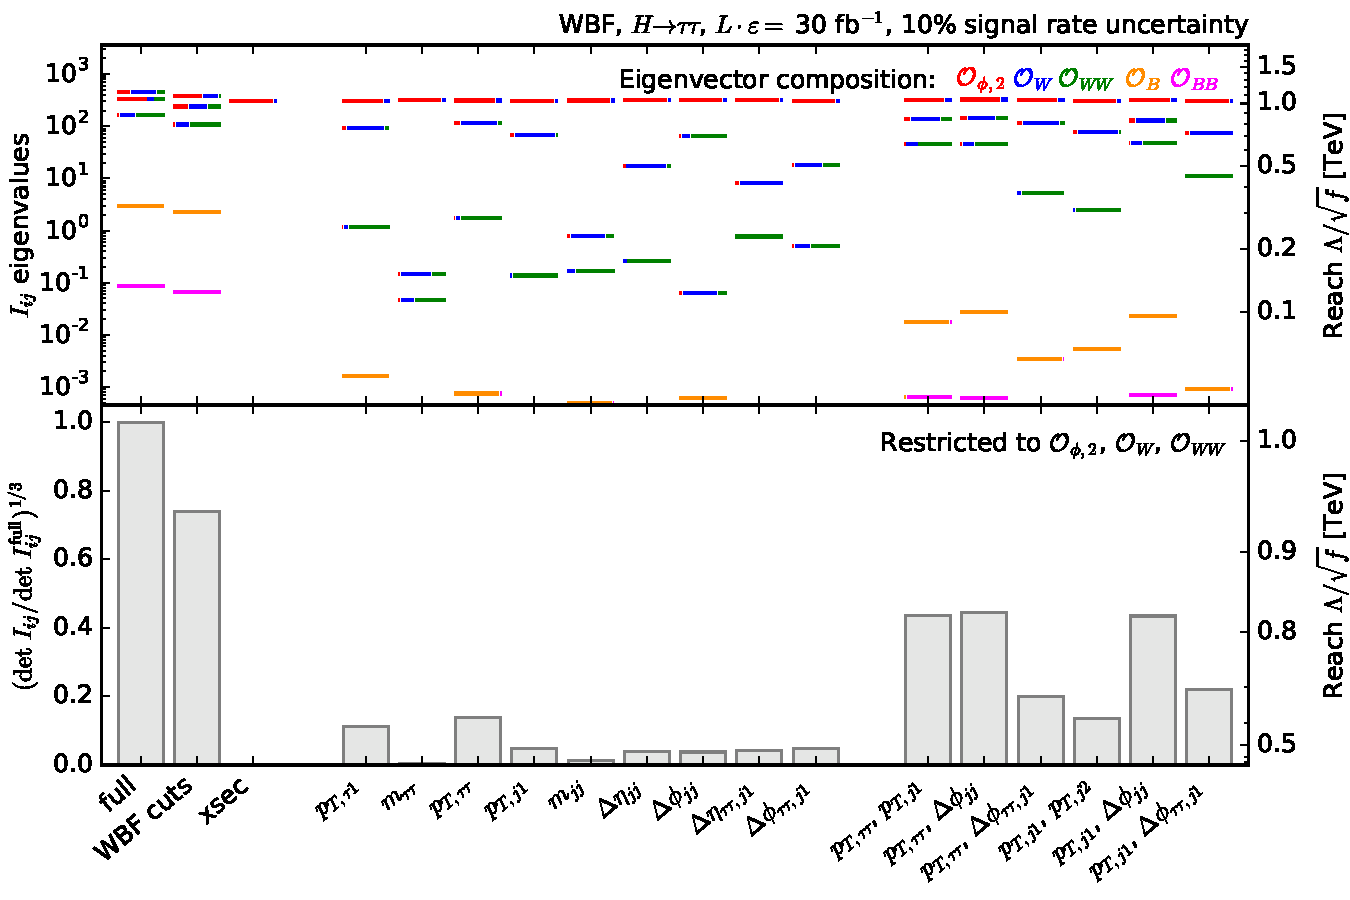
\includegraphics[width= \textwidth]{fig/information/wbf_tautau_histos_comparison_systematics.pdf}
  \caption{Fisher information for the WBF $h \to \tau \tau$ channel
    profiled over a $10\%$ signal rate uncertainty. We compare the
    total Fisher information, the information after the cuts in
    \autoref{eq:information_wbf_tautau_wbfcuts}, and the information
    in several distributions after this selection.  The top panel
    shows the eigenvalues, the colours denote the composition of the
    corresponding eigenvectors. The right axis translates the
    eigenvalues into a new physics reach for the corresponding
    combination of Wilson coefficients.  In the bottom panel we show
    the determinants of the Fisher information restricted to
    $\ope{\phi,2}$, $\ope{W}$, and $\ope{WW}$, normalised to the full
    information. Again, the right axis translates them into a new
    physics reach.}
  \label{fig:information_wbf_tautau_systematics_comparison}
\end{figure}

This treatment of systematic uncertainties on total rates can easily
be extended to phase-space-dependent effects, for instance
representing how the accuracy of the parton shower or the size of
missing higher-order corrections depend on the energy scale. This
requires parametrised smearing functions and an interpolation of the
differential cross sections between different benchmark values of the
nuisance parameters.




%%%%%%%%%%%%%%%%%%%%%%%%%%%%%%%%%%%%%%%%%%%%%%%%%%%%%%%%%%%%
\subsection{Comparison with other tools}
\label{sec:information_comparison}
%%%%%%%%%%%%%%%%%%%%%%%%%%%%%%%%%%%%%%%%%%%%%%%%%%%%%%%%%%%%

%%%%%%%%%%%%%%%%%%%%%%%%%%%%%%%%%%%%%%%%%%%%%%%%%%%%%%%%%%%%
\subsubsection{Likelihood ratio}
%%%%%%%%%%%%%%%%%%%%%%%%%%%%%%%%%%%%%%%%%%%%%%%%%%%%%%%%%%%%

There is a certain ambiguity in what constitutes an optimal
measurement. The aim of our approach is to minimise the covariance
matrix of estimators, which the Cram\'er-Rao bound links to the Fisher
information. Alternatively one can maximise the power of hypothesis
tests at a given significance level. According to the Neyman-Pearson
lemma, the relevant object is the (log) likelihood ratio between the
two hypotheses. These two objects are designed for different
questions: the likelihood ratio compares two discrete hypotheses,
while the Fisher information is suited for continuous parameter spaces
of arbitrary dimensionality.

We consider the expected log likelihood ratio
%
\begin{equation}
  q(\boldtheta_b , \boldtheta_a )
  \equiv -2 \, E \left[
  \log \frac { f(\mathbf{x}|\boldtheta_b) }   { f(\mathbf{x} |\boldtheta_a) }
  \middle | \boldtheta_a \right] \,.
\end{equation}
%
For the extended likelihood ansatz of \autoref{eq:information_extended_likelihood}, a brief calculation gives the likelihood ratio as
%
\begin{equation}
  q(\boldtheta_b , \boldtheta_a ) = -2 \, \sigma(\boldtheta_a) L \left( 1 - \frac {\sigma(\boldtheta_b)} {\sigma(\boldtheta_a)} + \log  \frac {\sigma(\boldtheta_b)} {\sigma(\boldtheta_a)} \right)
   -2 \,  \sigma(\boldtheta_a) L \;
    E \left[
    \log \frac { f^{(1)} (x|\boldtheta_b) }     { f^{(1)} (x|\boldtheta_a) }
    \middle | \boldtheta_a \right] \,.
\end{equation} 
%
This can be calculated with Monte-Carlo integration as given in
\autoref{eq:information_monte_carlo_integration}, finally leading to
%
\begin{equation}
  q(\boldtheta_b , \boldtheta_a ) = -2 \,  L \; \sum_{\text{events}} \;
  \Delta \sigma (\boldtheta_a)  \;
  \log \frac {\Delta \sigma (\boldtheta_b) } { \Delta \sigma (\boldtheta_a) } \,.
\end{equation}

With this result we can compare the log likelihood ratio to the
distances defined by information geometry. For WBF Higgs production in
the $\tau \tau$ mode as described in
\autoref{sec:information_wbf_tautau}, we sample parameter points
$\boldtheta$ in the $\ope{W}$-$\ope{WW}$ plane. For each of these
points we calculate the local and global distance from the SM point
defined by the Fisher information, as well as the expected
log-likelihood ratio
%
\begin{align}
  q(\boldtheta_b , \boldtheta_a )
  \equiv -2 \, E \left[
  \log \frac { f(\mathbf{x}|\boldtheta_b) }   { f(\mathbf{x} |\boldtheta_a) }
  \middle | \boldtheta_a \right] \,.
\end{align}

\begin{figure}
  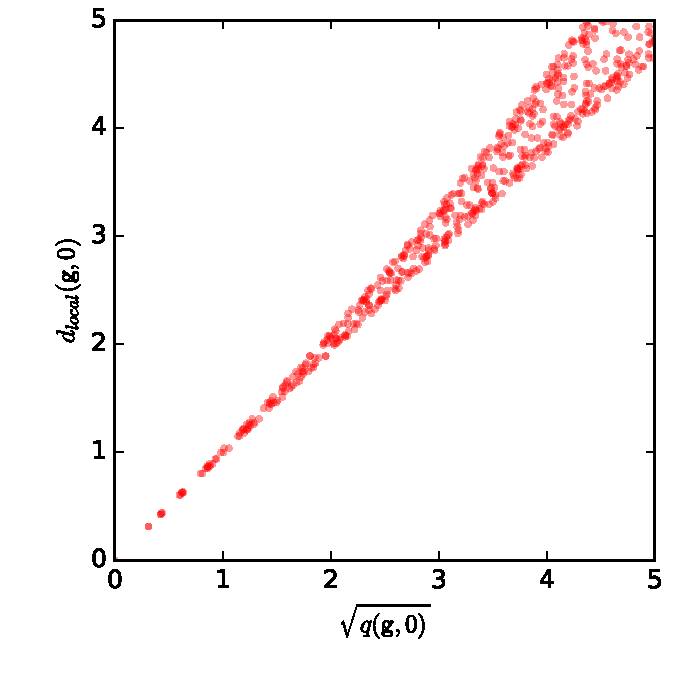
\includegraphics[width=0.49 \textwidth]{fig/information/wbf_tautau_local_distance_vs_llr}%
  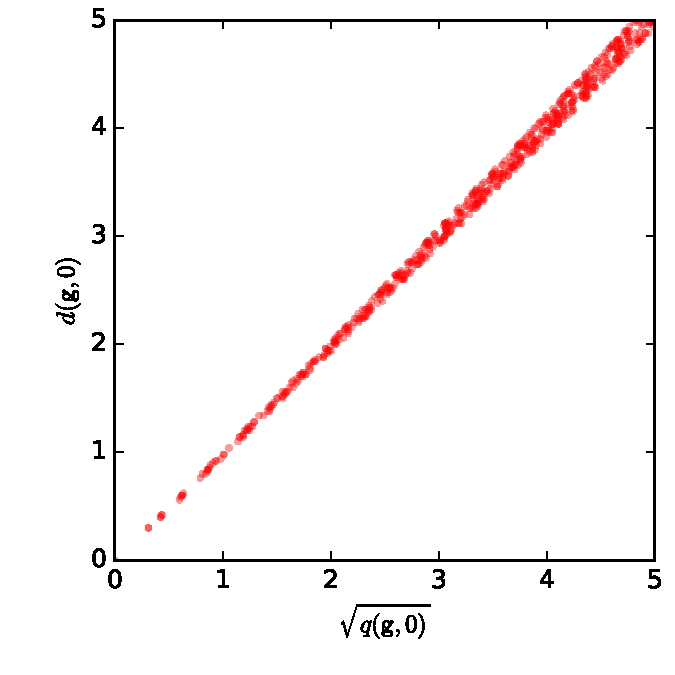
\includegraphics[width=0.49 \textwidth]{fig/information/wbf_tautau_distance_vs_llr}%
  \caption{Comparison of the local (left) and global (right) distances
    defined by the Fisher information with the expected local
    likelihood ratio. We use WBF Higgs production in the $\tau \tau$
    mode and sample parameter points in the $\ope{W}$-$\ope{WW}$
    plane.}
  \label{fig:information_wbf_tautau_llr}
\end{figure}

As shown in \autoref{fig:information_wbf_tautau_llr}, the local and
especially the global distances are almost exactly equal to the
expected likelihood ratio, with small differences only becoming
visible around the $3 \sigma$ level.  This demonstrates that different
statistical tools probe the same physics and can be chosen based on
practical considerations. In particular, the conclusions from an
information-based analysis, utilising the convenient properties for
high-dimensional theory spaces, also apply to exclusion limits based
on the log likelihood ratio.



%%%%%%%%%%%%%%%%%%%%%%%%%%%%%%%%%%%%%%%%%%%%%%%%%%%%%%%%%%%%
\subsubsection{Ambient Fisher information}
%%%%%%%%%%%%%%%%%%%%%%%%%%%%%%%%%%%%%%%%%%%%%%%%%%%%%%%%%%%%

Information geometry, as introduced in
\autoref{sec:information_formalism}, assigns structure to the
parameter space of a theory. It is, interestingly, possible to define
a distance measure in the space of \emph{all} distributions, without
relying on any model structure. One such approach is the \emph{ambient
  Fisher information}~\cite{dawid1977, carter2008}. It defines the
distance between two distributions $f_a(\boldx)$ and
$f_b(\boldx)$ as
%
\begin{equation}
  d_{\text{ambient}} (f_a, f_b) = \arccos \intfatx  \sqrt {f_a(\boldx) f_b(\boldx)} \,.
  \label{eq:information_ambient_distance}
\end{equation}
%
This measure does not require an integration along model
parameters. As long as the distributions $f_a$ and $f_b$ are similar
or the distances small, it approaches the usual global distance of
information geometry~\cite{carter2008}:
%
\begin{equation}
  2 \, d_{\text{ambient}} (f(\boldx|\boldtheta_a), f(\boldx|\boldtheta_b)) \sim d(\boldtheta_a, \boldtheta_b) \,.
  \label{eq:information_ambient_equivalence}
\end{equation}
%
For this reason, distances based on the ambient Fisher information
have been suggested as a computationally less expensive approximation
for information distances~\cite{carter2008}. 

\begin{figure}
  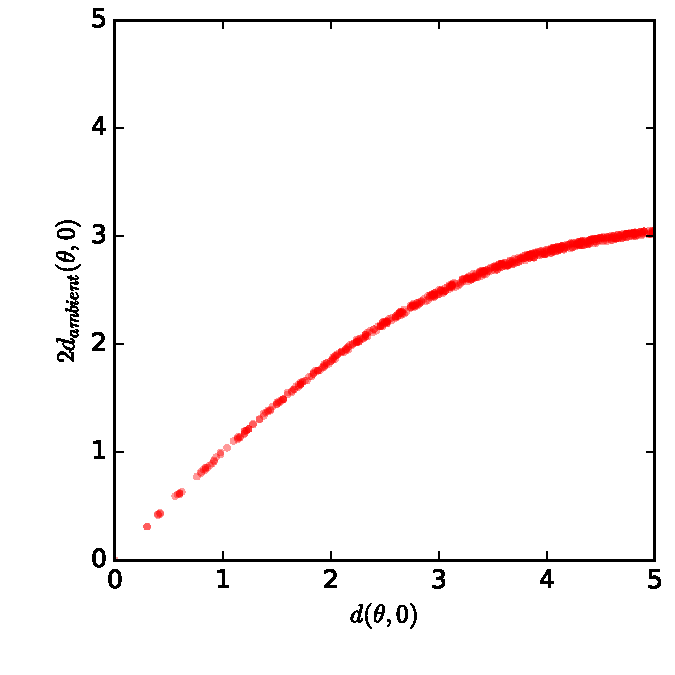
\includegraphics[width=0.49 \textwidth]{fig/information/wbf_tautau_ambient}
  \caption{Comparison of the distance according to the ambient Fisher
    geometry, defined in \autoref{eq:information_ambient_distance}, to
    the distance defined by the usual Fisher information on the theory
    space. We use WBF Higgs production in the $\tau \tau$ mode and
    sample parameter points in the $\ope{W}$-$\ope{WW}$ plane.}
  \label{fig:information_wbf_tautau_ambient}
\end{figure}

In \autoref{fig:information_wbf_tautau_ambient} we compare this tool
to our global distance measure. Again, we use the WBF $h\to \tau \tau$
channel as described in \autoref{sec:information_wbf_tautau} and sample
parameter points in the $\ope{W}$-$\ope{WW}$
plane. \autoref{eq:information_ambient_equivalence} holds at distances
up to $d \lesssim 2$, beyond which the two measures diverge, and the
ambient distance is ultimately limited from above at $\pi/2$.



%%%%%%%%%%%%%%%%%%%%%%%%%%%%%%%%%%%%%%%%%%%%%%%%%%%%%%%%%%%%
\section{Conclusions}
\label{sec:information_conclusions}
%%%%%%%%%%%%%%%%%%%%%%%%%%%%%%%%%%%%%%%%%%%%%%%%%%%%%%%%%%%%

% We introduced new statistical tools based on information geometry to
% optimise measurements of continuous theory parameters at the LHC.
% Our approach is based on the Fisher information matrix. Following
% the Cram\'er-Rao bound, it defines the maximum precision with which
% model parameters can be estimated. It is well-suited to
% high-dimensional parameter spaces since it requires no
% discretisation of the tested hypotheses, does not depend on
% arbitrary basis choices, and can simultaneously encode the maximum
% sensitivity to all directions in model space in a single
% matrix. These properties make information geometry particularly
% useful for the analysis of effective field theories. Moreover, the
% Fisher information is additive between different measurements and
% between different phase-space region within the same process, making
% it trivial to discuss the combination of different
% channels. Understood as a metric on the theory space, it provides an
% intuitive geometric interpretation of discrimination power.

Information geometry can be used to optimise measurements of any set
of continuous theory parameters at the LHC. Following the Cram\'er-Rao
bound, the Fisher information matrix defines the maximum precision
with which model parameters can be estimated. It is well-suited to
high-dimensional parameter spaces since it requires no discretisation
of the tested hypotheses, does not depend on arbitrary basis choices,
and can simultaneously encode the maximum sensitivity to all
directions in model space in a single matrix. These properties make
information geometry particularly useful for the analysis of effective
field theories. Moreover, the Fisher information is additive between
different measurements and between different phase-space region within
the same process, making it trivial to discuss the combination of
different channels. Understood as a metric on the theory space, it
provides an intuitive geometric interpretation of discrimination
power.

We developed an algorithm that can calculate the Fisher information in
arbitrary high-energy physics processes based on Monte-Carlo
simulations. We can calculate the total information based on the full
high-dimensional phase space with all correlations. This defines the
maximal precision with which the parameters can be probed; applied to
effective field theories this gives us the maximal new physics reach
of any signature. The Fisher information can also be calculated
differentially to understand how the discriminating power is
distributed over phase space, helping to define optimal event
selection. Alternatively, we can calculate the information in
individual distributions of kinematic observables rather than the full
high-dimensional kinematics. This defines the most powerful
observables, and lets us compare the power of simple histogram-based
analyses to methods based on the matrix elements or machine-learning
techniques. All of these instruments can be useful to improve
measurement strategies. An interesting feature of the geometric
interpretation is that the curvature of the Riemannian manifold
defined by the Fisher information provides a handle on the square of
dimension-six contributions. As discussed in
\autoref{sec:validity_squares}, under certain assumptions this lets us
analyse the convergence of the EFT expansion in $1/\Lambda$.

With these novel tools we analysed how well effective dimension-six
operators can be measured in three different Higgs channels. First, we
studied the kinematics of Higgs production in weak boson fusion with a
decay into a tau pair.  As expected, a large fraction of the
constraining power in this process comes from few events with large
momentum transfer. Care has to be taken with tight cuts on the
rapidity separation of the tagging jets, which throw away a large
amount of discrimination power. Different kinematic observables probe
different directions in theory space: transverse momenta of the
final-state particles, for instance the tagging jets, generally probe
$\ope{W}$, while the only standard observable with a large sensitivity
to $\ope{WW}$ is the azimuthal angle between the tagging jets. To
facilitate the most powerful and flexible interpretation of their
results, the experimental collaborations should ideally measure and
publish the fully correlated two-dimensional histogram between these
two quantities. Under idealised conditions, the analysis of such a
two-dimensional histogram can probe new physics scales around
$1.1~\tev$ in the $\ope{W}$-$\ope{WW}$-$\ope{\phi,2}$ space in the
early phase of Run~2. Fully multivariate analyses have the potential
to further enhance the sensitivity and probe new physics scales of up
to $1.2~\tev$.

Our next example process was Higgs production with a $h \to 4 \ell$
decay, a very clean signature with rich kinematics. We used it to
compare the sensitivity to dimension-six physics in the decay and
production vertices within the same process. Our results are
unambiguous: the decay kinematics is much less sensitive to
momentum-dependent operators than the production-side probes provided
by the tagging jets. This reflects the $E^2/\Lambda^2$ dependency of
such dimension-six effects, which can be large in the production
vertex, while the momentum flow through the decay vertex is limited to
the Higgs mass.

Higgs production in association with a single top has an interesting
amplitude structure where diagrams with Higgs-gauge interactions
interfere destructively with diagrams depending on the top Yukawa
coupling. Small changes to these interactions can in principle change
the total production rate and the kinematics drastically. We showed
that kinematic properties of the Higgs decay products and observables
related to the top system provide orthogonal information on the theory
space; in particular the diphoton transverse momentum as well as the
rapidity separation of the $\gamma \gamma$ and the $bjj$ system
provide useful information.  Unfortunately, the tiny cross section of
this process strongly limits the constraining power on dimension-six
operators. Even with HL-LHC data and under idealised conditions, these
distributions are only sensitive to new physics scales around
$550~\gev$, while an optical multivariate analysis may be able to
probe scales up to $700~\gev$ according to the Cram\'er-Rao bound.

These initial studies do not include systematic and theory
uncertainties, and detector effects are taken into account only with
rudimentary smearing functions. Our results for the maximum precision
are therefore optimistic. We showed how our approach can be extended
to include systematic effects, and introduced a profiling procedure
for the Fisher information. These tools define many directions for
future research. First, the Higgs signatures discussed here can be
re-examined with a proper treatment of shower and detector effects as
well as systematic and theory uncertainties. Second, we can analyse
the detection of $CP$ violation in the Higgs sector. Using the
profiling procedure for the Fisher information, we can focus on the
question which signatures of $CP$ violation are genuine, \ie cannot be
caused by any $CP$-conserving new physics. Finally, while we focussed
on Higgs physics in terms of effective field theories in this thesis,
these tools can be applied to the measurement of any continous
parameters in any perturbative LHC signature.
